\documentclass[hyperref={pdfpagelabels=false}]{beamer}
% beamer already loads hyperref; do NOT load \usepackage{hyperref} again.

\usepackage{ragged2e} % 文字向兩邊對齊
\renewcommand{\raggedright}{\leftskip=0pt \rightskip=0pt plus 0cm}

\usepackage{listings}
\usepackage{lmodern}
\usepackage{fontspec}
\usepackage{xeCJK}
\setCJKmainfont{Noto Sans CJK TC}
%（可選）若你會用到無襯線中文或等寬中文，建議補上：
\setCJKsansfont{Noto Sans CJK TC}
\setCJKmonofont{Noto Sans Mono CJK TC}

\usepackage[english]{babel}
\usepackage{amsmath,amssymb,amsfonts,amsthm}

% hyperref settings (since beamer already loads hyperref)
\hypersetup{
  colorlinks=true,
  urlcolor=blue,
  citecolor=blue,
  pdfborder={0 0 0}
}

\usepackage{accsupp}% http://ctan.org/pkg/accsupp
\newcommand{\emptyaccsupp}[1]{\BeginAccSupp{ActualText={}}#1\EndAccSupp{}}

\usepackage{tikz}
\usetikzlibrary{arrows,decorations.pathmorphing,backgrounds,fit,positioning,shapes.symbols,chains}

\usepackage{booktabs}
\usepackage{threeparttable}
\usepackage{colortbl} 
\usepackage{xcolor}
\usetikzlibrary{tikzmark}

\newcommand{\indep}{\perp\!\!\!\perp}
\newcommand{\nindep}{\not\!\perp\!\!\!\perp}

\beamertemplatefootpagenumber


\usepackage{listings}
%%%%%%%%%%%%%%%%%%%%%%%%%%%%%%%%%%%%%%%%%%%%%%%%%%%%%%%%%%%%%%%%%%%%%%%%%%%%%%
% LaTeX snippet: language and style definition of Stata for listings package.
%                [listings](http://www.ctan.org/pkg/listings) 
%                [Stata](http://www.stata.com/)
%
% Usage:
%     Copy the code into your preamble, or import it by `\include` .
%     then in your doc:
%     \lstinputlisting[style=numbers]{DO-SCRIPT}
%     \lstinputlisting[style=numbers, style=stata-editor]{DO-SCRIPT}
%     \lstinputlisting[style=nonumbers, frame=none]{DO-SCRIPT}
% How it works:
%     - The language is defined by `\lstdefinelanguage{Stata}`
%     - Four styles is defined by `\lstdefinestyle{STYLE-NAME}`, 
%       they are: numbers and no numbers, plain(black and white) and colorful
%       (colored roughly like stata editor.)
% Tips:
%     - Generally you only need to set your default in the last part,
%       that is, code inside of `\lstset`.
%     - Add more keywords(I can not list all of them) in the `\lstset` part.
%     - Do NOT leave any blank lines in commands
%       (`\lstddefinelanguage', `\lstdefinestyle` and `\lstset`)
%
% update: 2014-04-16
% version: 0.1
% author: kongs
% licence: MIT
% url: https://gist.github.com/kongs-sublime/10862838
%
% TODO: 
%       - finish keyword list.
%       - precise colors that match stata editor?
%       - make it flexible(fonts and style)
%
%%%%%%%%%%%%%%%%%%%%%%%%%%%%%%%%%%%%%%%%%%%%%%%%%%%%%%%%%%%%%%%%%%%%%%%%%%%%%%


% langugae defination
\lstdefinelanguage{Stata}{
	% Left for users to add missing commands,
	% with possibility of choosing different style.
	morekeywords=,
	% Popular add-on commands
	morekeywords=[2]{cntrade, chinafin, 
		wbopendata, spmap,
	},
	% System commands
	morekeywords=[3]{regress, summarize, 
		display,
	},
	% Keywords
	morekeywords=[4]{forvalues, if, foreach, set},
	% Built-in functions
	morekeywords=[5]{rnormal, runiform},
	morecomment=[l]{//},
	% morecomment=[l]{*},  // `*` maybe used as multiply operator. So use `//` as line comment.
	morecomment=[s]{/*}{*/},
	% morecomment=[s]{,}{//},
	% The following is used by macros, like `lags'.
	morecomment=[n][keywordstyle9]{`}{'},
	morestring=[b]",
	sensitive=true,
}

\lstdefinestyle{numbers}{
	numbers=left, 
	stepnumber=1, 
	numberstyle=\tiny\emptyaccsupp,
	xleftmargin=2em,
}

\lstdefinestyle{nonumbers}{
	numbers=none,
}

\lstdefinestyle{stata-plain}{
	language=Stata,
	basicstyle=\footnotesize\ttfamily,
}

\lstdefinestyle{stata-editor}{
	language=Stata,
	basicstyle=\footnotesize\ttfamily,  
	keywordstyle={\color{NavyBlue}},  
	keywordstyle=[2]{\color{NavyBlue}},
	keywordstyle=[3]{\color{NavyBlue}},
	keywordstyle=[4]{\color{NavyBlue}},
	keywordstyle=[5]{\color{Blue}},
	keywordstyle=[9]{\color{TealBlue}},
	stringstyle=\color{Maroon},
	commentstyle=\color{OliveGreen},
}

\lstset{
	language=Stata,
	style=stata-plain,
	% style=stata-editor,
	style=numbers,
	showstringspaces=false,
	breaklines,
	frame=single,
	% To add missing commands
	% morekeywords={xtreg, xtunitroot},
}




\title[]  
{Spatial Data in Economics}

%\subtitle
%{免除部分負擔對幼兒醫療利用與健康的影響:斷點迴歸分析}

%\author 
 %{Tzu-Ting Yang\inst{1} \and Hsing-Wen Han\inst{2} \and Hsien-Ming Lien\inst{3}}

%\institute[short]{\inst{1} Academia Sinica \and \inst{2} Tamkang University \and \inst{3} National Chengchi University}


%\author 
 %{Prof. Tzu-Ting Yang}

%\institute{Institute of Economics, Academia Sinica  \\ Econ, NTU}
%\institute{Institute of Economics, Academia Sinica  \\ IMES/IDAS, NCCU}
%\institute{Institute of Economics, Academia Sinica}


\author 
{Prof. Tzu-Ting Yang  \\ 楊子霆}

%\institute{Institute of Economics, Academia Sinica  \\ Econ, NTU}
\institute{Institute of Economics, Academia Sinica  \\ 中央研究院經濟研究所}
%\institute{Institute of Economics, Academia Sinica  \\ Econ, NTU}
%\institute{Institute of Economics, Academia Sinica  \\ IMES/IDAS, NCCU}

%\author 
%{楊子霆 \\ 中研院經濟所}

%\institute 
%{中正大學國際經濟專題研討}




\date
{\today}



% \usetheme{CambridgeUS}
% %\usecolortheme{seahorse}
% \setbeamertemplate{footline}{%
% 	\hfill\usebeamercolor[fg]{page number in head/foot}%
% 	\usebeamerfont{page number in head/foot}%
% 	\insertframenumber\,/\,\inserttotalframenumber\hspace{1em}\vspace{2pt}%
% }

\usetheme{Boadilla}
%\useinnertheme{rectangles}

%\usetheme{CambridgeUS}
\usecolortheme{seahorse}
\setbeamertemplate{footline}{%
	\hfill\usebeamercolor[fg]{page number in head/foot}%
	\usebeamerfont{page number in head/foot}%
	\insertframenumber\,/\,\inserttotalframenumber\hspace{1em}\vspace{2pt}%
}


% \usepackage{beamerthemeshadow}
% %\usecolortheme{seahorse}
% \setbeamertemplate{footline}{%
% 	\hfill\usebeamercolor[fg]{page number in head/foot}%
% 	\usebeamerfont{page number in head/foot}%
% 	\insertframenumber\,/\,\inserttotalframenumber\hspace{1em}\vspace{2pt}%
% }



%\useinnertheme{rectangles}

%\usepackage{beamerthemeshadow}
\beamersetuncovermixins{\opaqueness<1>{25}}{\opaqueness<2->{15}}

\begin{document}
	
	
	\begin{frame}{}
	\titlepage
\end{frame}






\title[]  
{Overview}


\author 
{}

%\institute{Institute of Economics, Academia Sinica  \\ Econ, NTU}
%\institute{Institute of Economics, Academia Sinica  \\ IMES/IDAS, NCCU}
\institute{}

%\author 
%{楊子霆 \\ 中研院經濟所}

%\institute 
%{中正大學國際經濟專題研討}




\date
{}


\begin{frame}{}
	\titlepage
\end{frame}





% \begin{frame}{Why GIS for Economists?}{}
% \begin{itemize}
% 	\item The use of geographic information system (GIS) has
% 	increasingly been popular among economists
% 	\vspace{0.2cm}
% 	\item There are at least two reasons for this popularity
% 	\vspace{0.2cm}
% 	\item[1] GIS allows economists to observe the previously unobserved	and makes research feasible
% 	\vspace{0.2cm}
% 	\begin{itemize}
% 		\item Satellite images
% 		\vspace{0.2cm}
% 		\item Scanned old maps
% 		\vspace{0.2cm}
% 	\end{itemize}
% 	\item[2] GIS helps economists identify causal impacts in a more credible way than previously possible
% 	\begin{itemize}
% 		\vspace{0.2cm}
% 		\item Distance
% 		\vspace{0.2cm}
% 		\item Elevation
% 		\vspace{0.2cm}
% 		\item Spatial regression discontinuity design
% 	\end{itemize} 
% \end{itemize}
% \end{frame}



% \begin{frame}{Make Research Feasible}{Example: Satellite Images}
% J. Vernon Henderson, Adam Storeygard, and David N. Weil (2012), ``\textbf{Measuring Economic Growth from Outer Space}", AER
% \begin{itemize}
% \vspace{0.2cm}
% \item They develop a statistical framework to use satellite data on night lights to estimate GDP growth
% \vspace{0.2cm}
% \begin{itemize}
% \item Their estimates are quite close to official growth data
% \vspace{0.2cm}
% \end{itemize}
% \item Using night lights data, empirical analyses of growth need no longer use countries as the unit of analysis
% \vspace{0.2cm}
% \begin{itemize}
% \item Measure growth for sub- and supranational regions
% \end{itemize}
% \end{itemize}
% \end{frame}


% \begin{frame}{Satellite Images}{World}
% 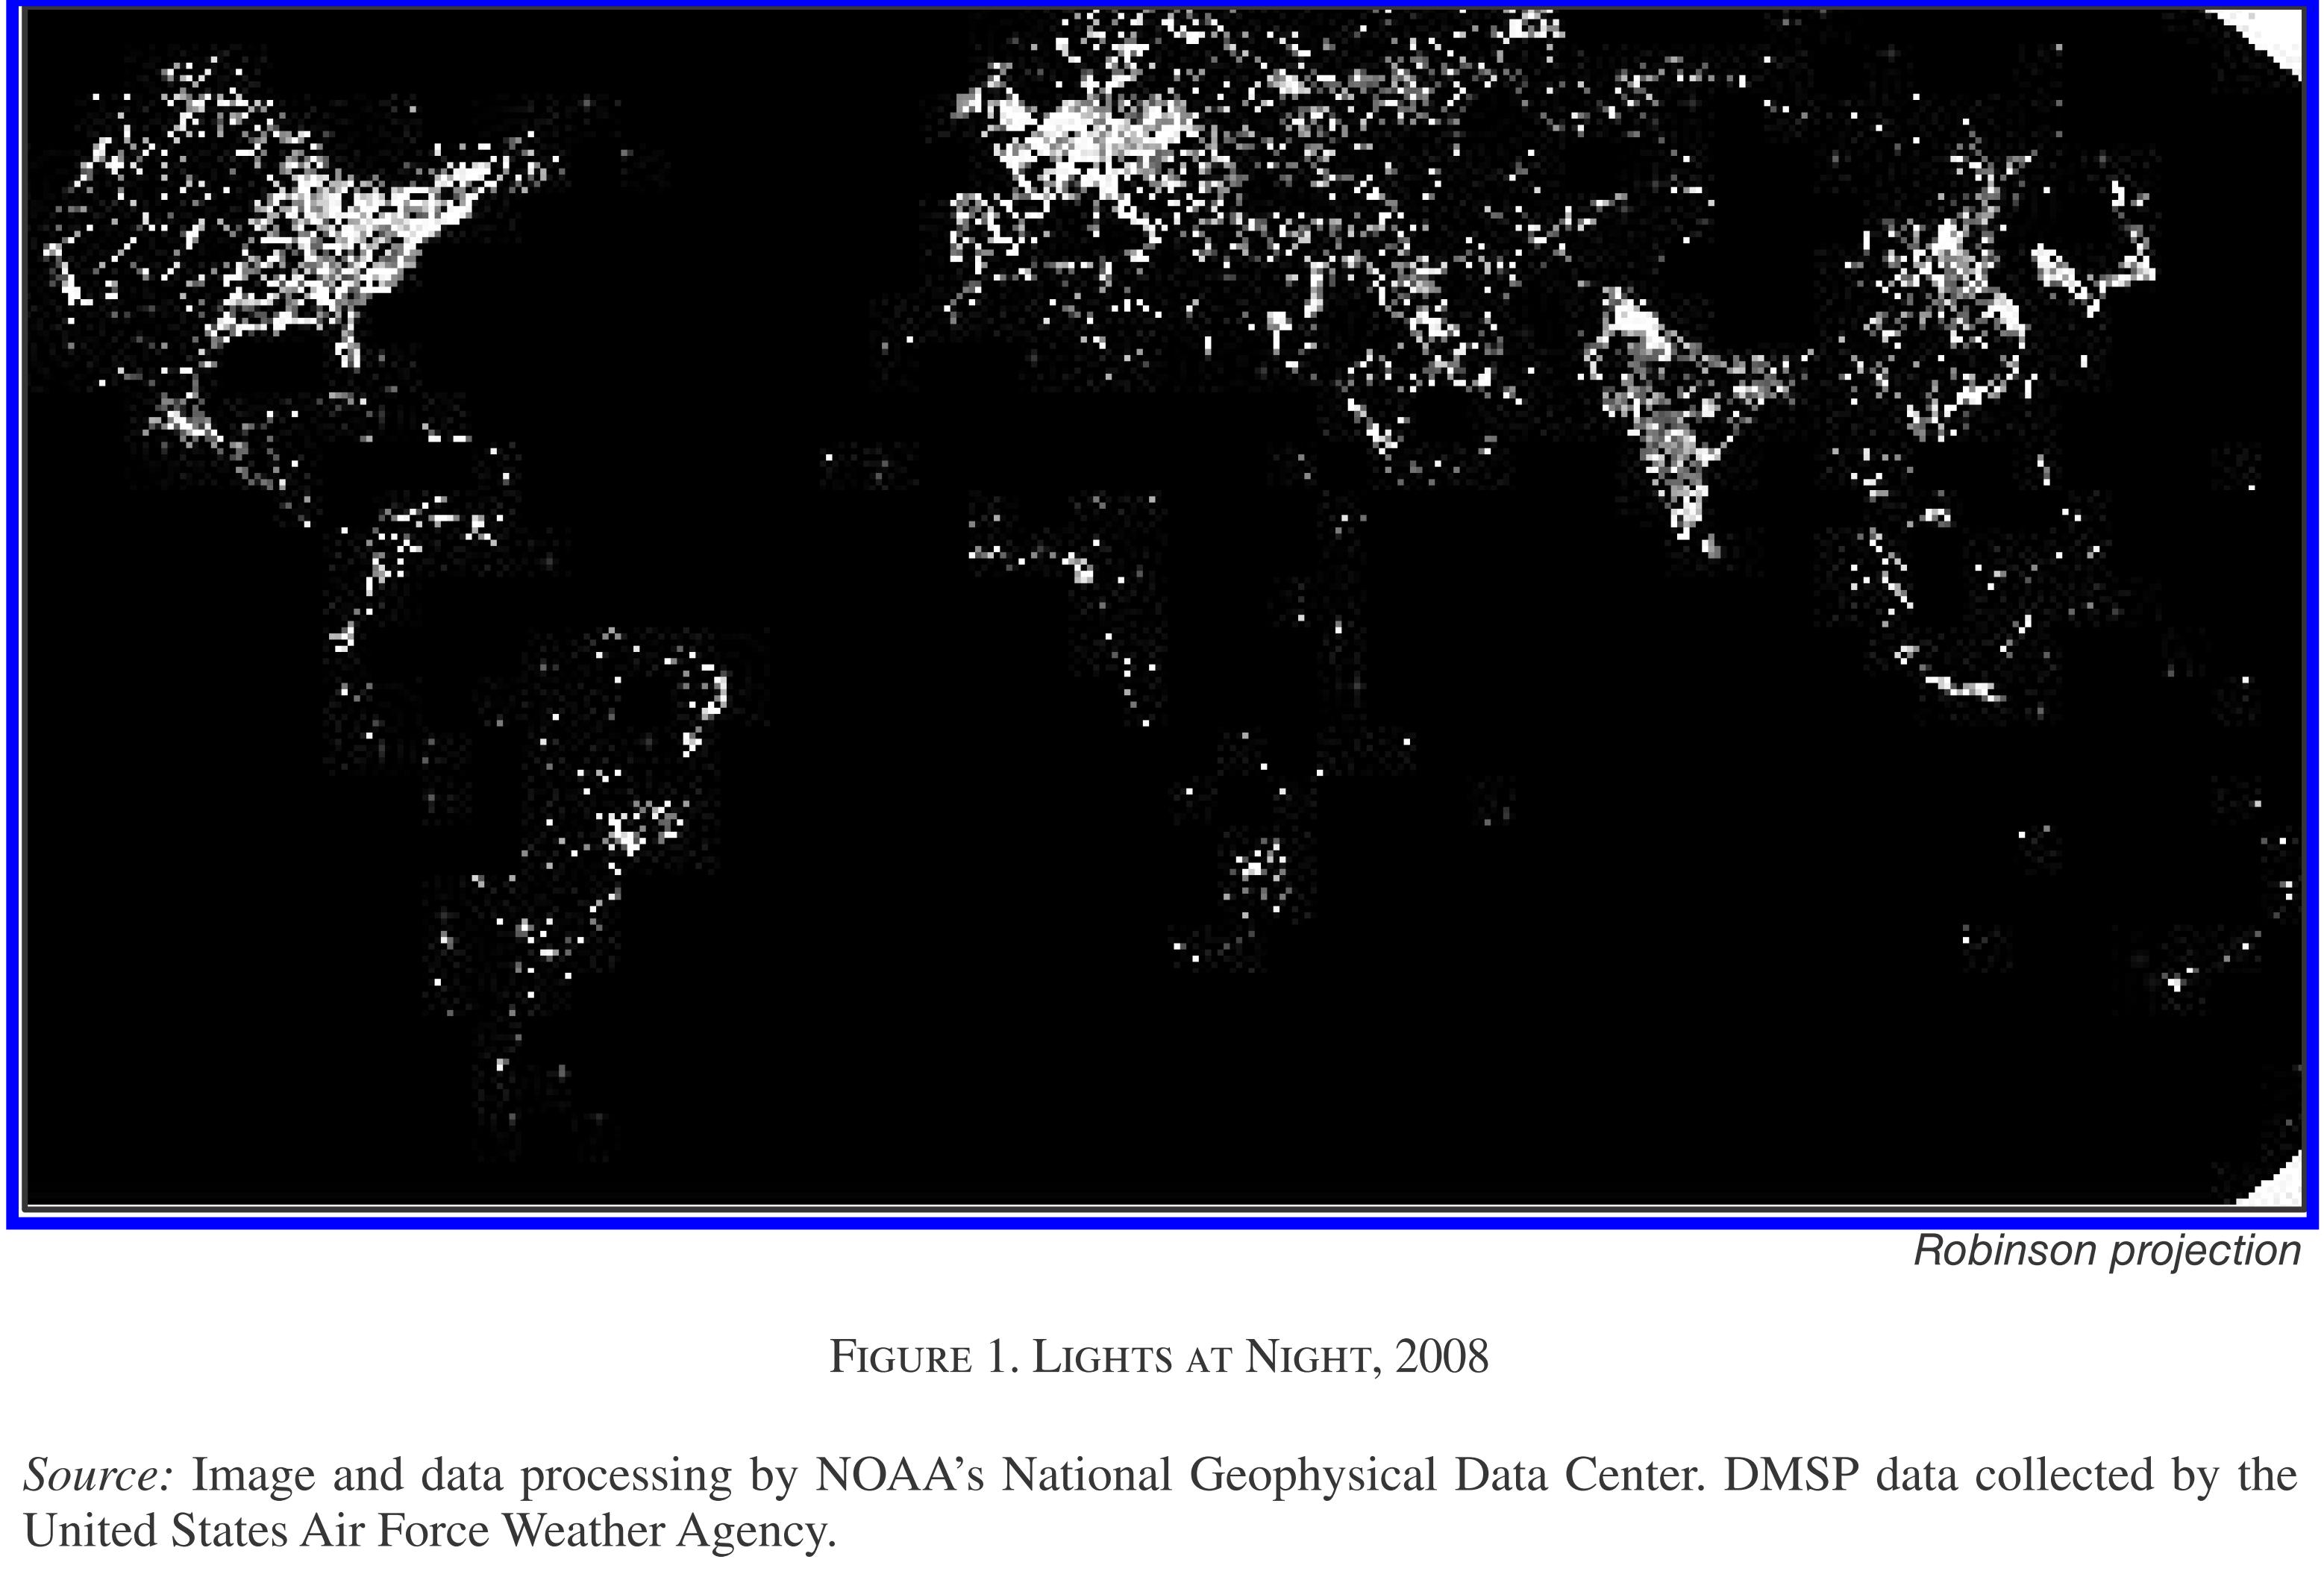
\includegraphics[width=0.9\textwidth]{figure/measure_g_f1.jpg}

% \end{frame}


% \begin{frame}{Satellite Images}{Long-Run Growth in Korea}
% 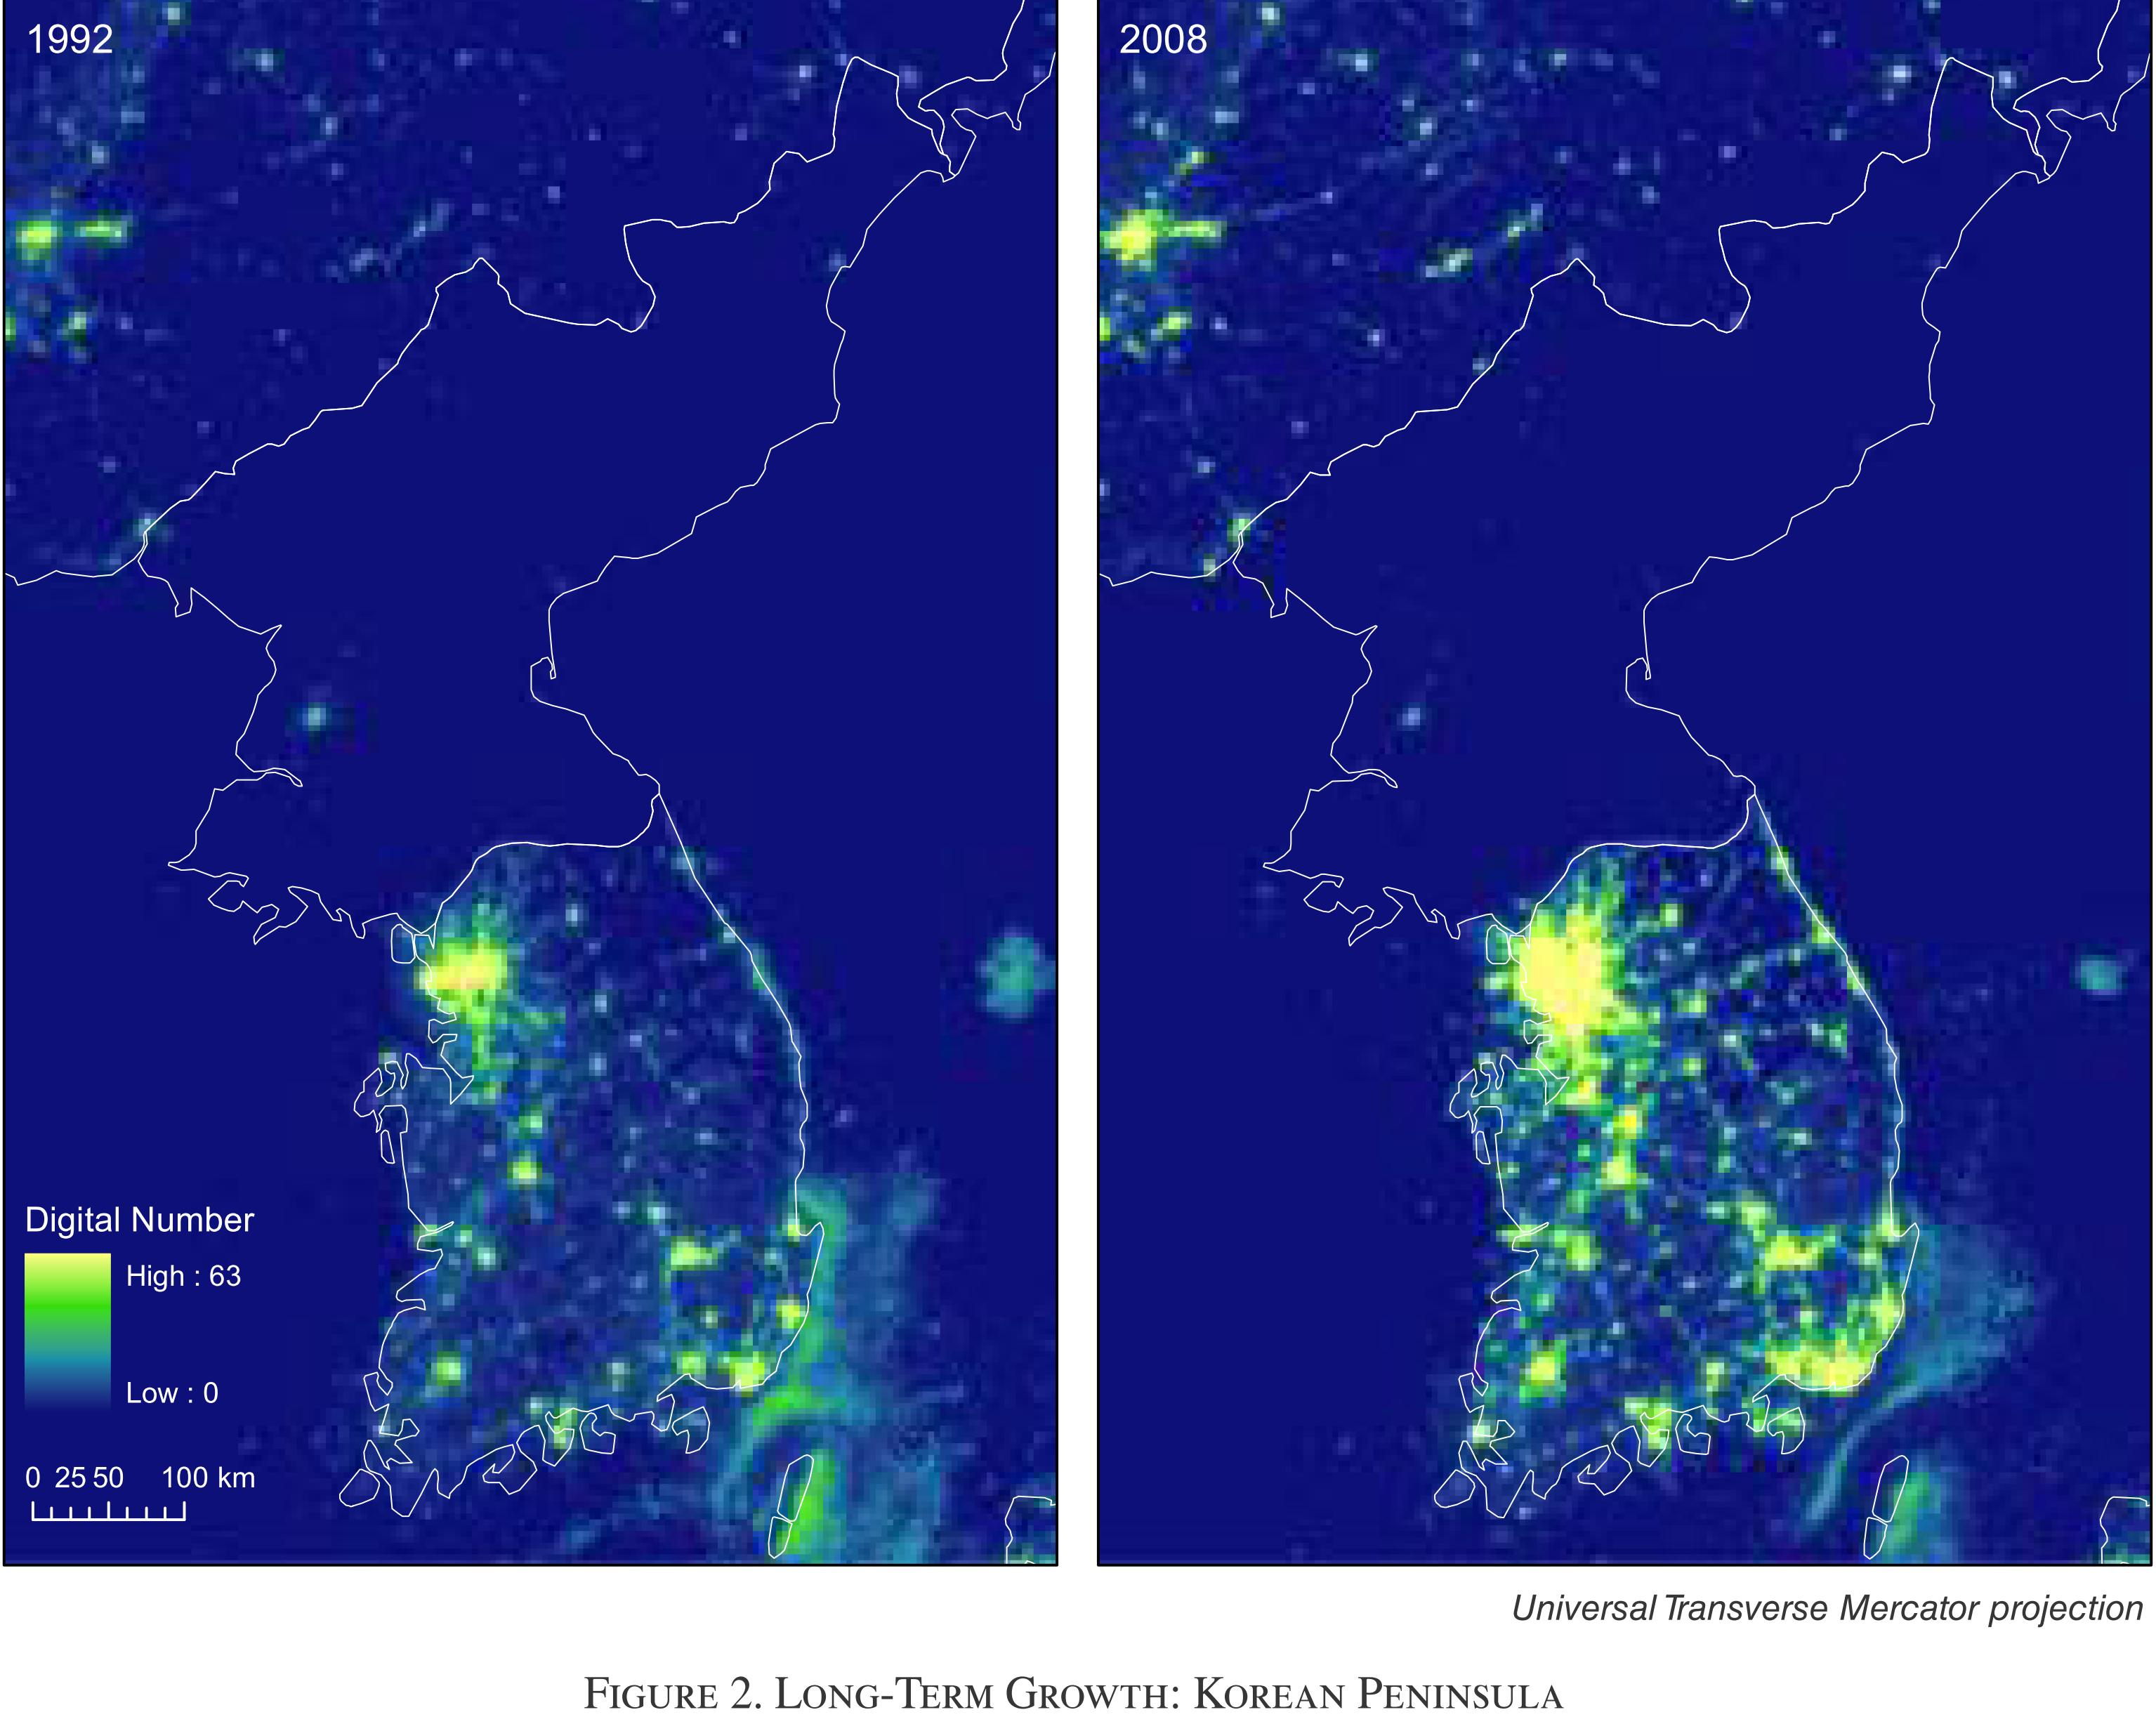
\includegraphics[width=0.9\textwidth]{figure/measure_g_f2.jpg}

% \end{frame}






% %districts that share the ethnicity of the president receive twice as much expenditure on roads and have five times the length of paved roads built



% \begin{frame}{Make Research Feasible}{Example: Scanned Old Maps}
% 	Robin Burgess, Remi Jedwab, Edward Miguel, 
% 	Ameet Morjaria, and Gerard Padr\'o i Miquel (2015), ``\textbf{The Value of Democracy: 
% 		Evidence from Road Building in Kenya}", AER
% 	\begin{itemize}
% 		\vspace{0.2cm}
% 		\item Did Kenyan presidents build more roads for their co-ethnics?
% 		\vspace{0.2cm}
% 		\begin{itemize}
% 			\item They digitalized the old maps to get the building of roads since the year of independence in Kenya (1961)
% 			\vspace{0.2cm}
% 			\item Track road network expansion over time
% 		\end{itemize}
% 	\end{itemize}
% \end{frame}




% \begin{frame}{Scanned Old Maps}{Map of Roads in Kenya in 1961}
% 	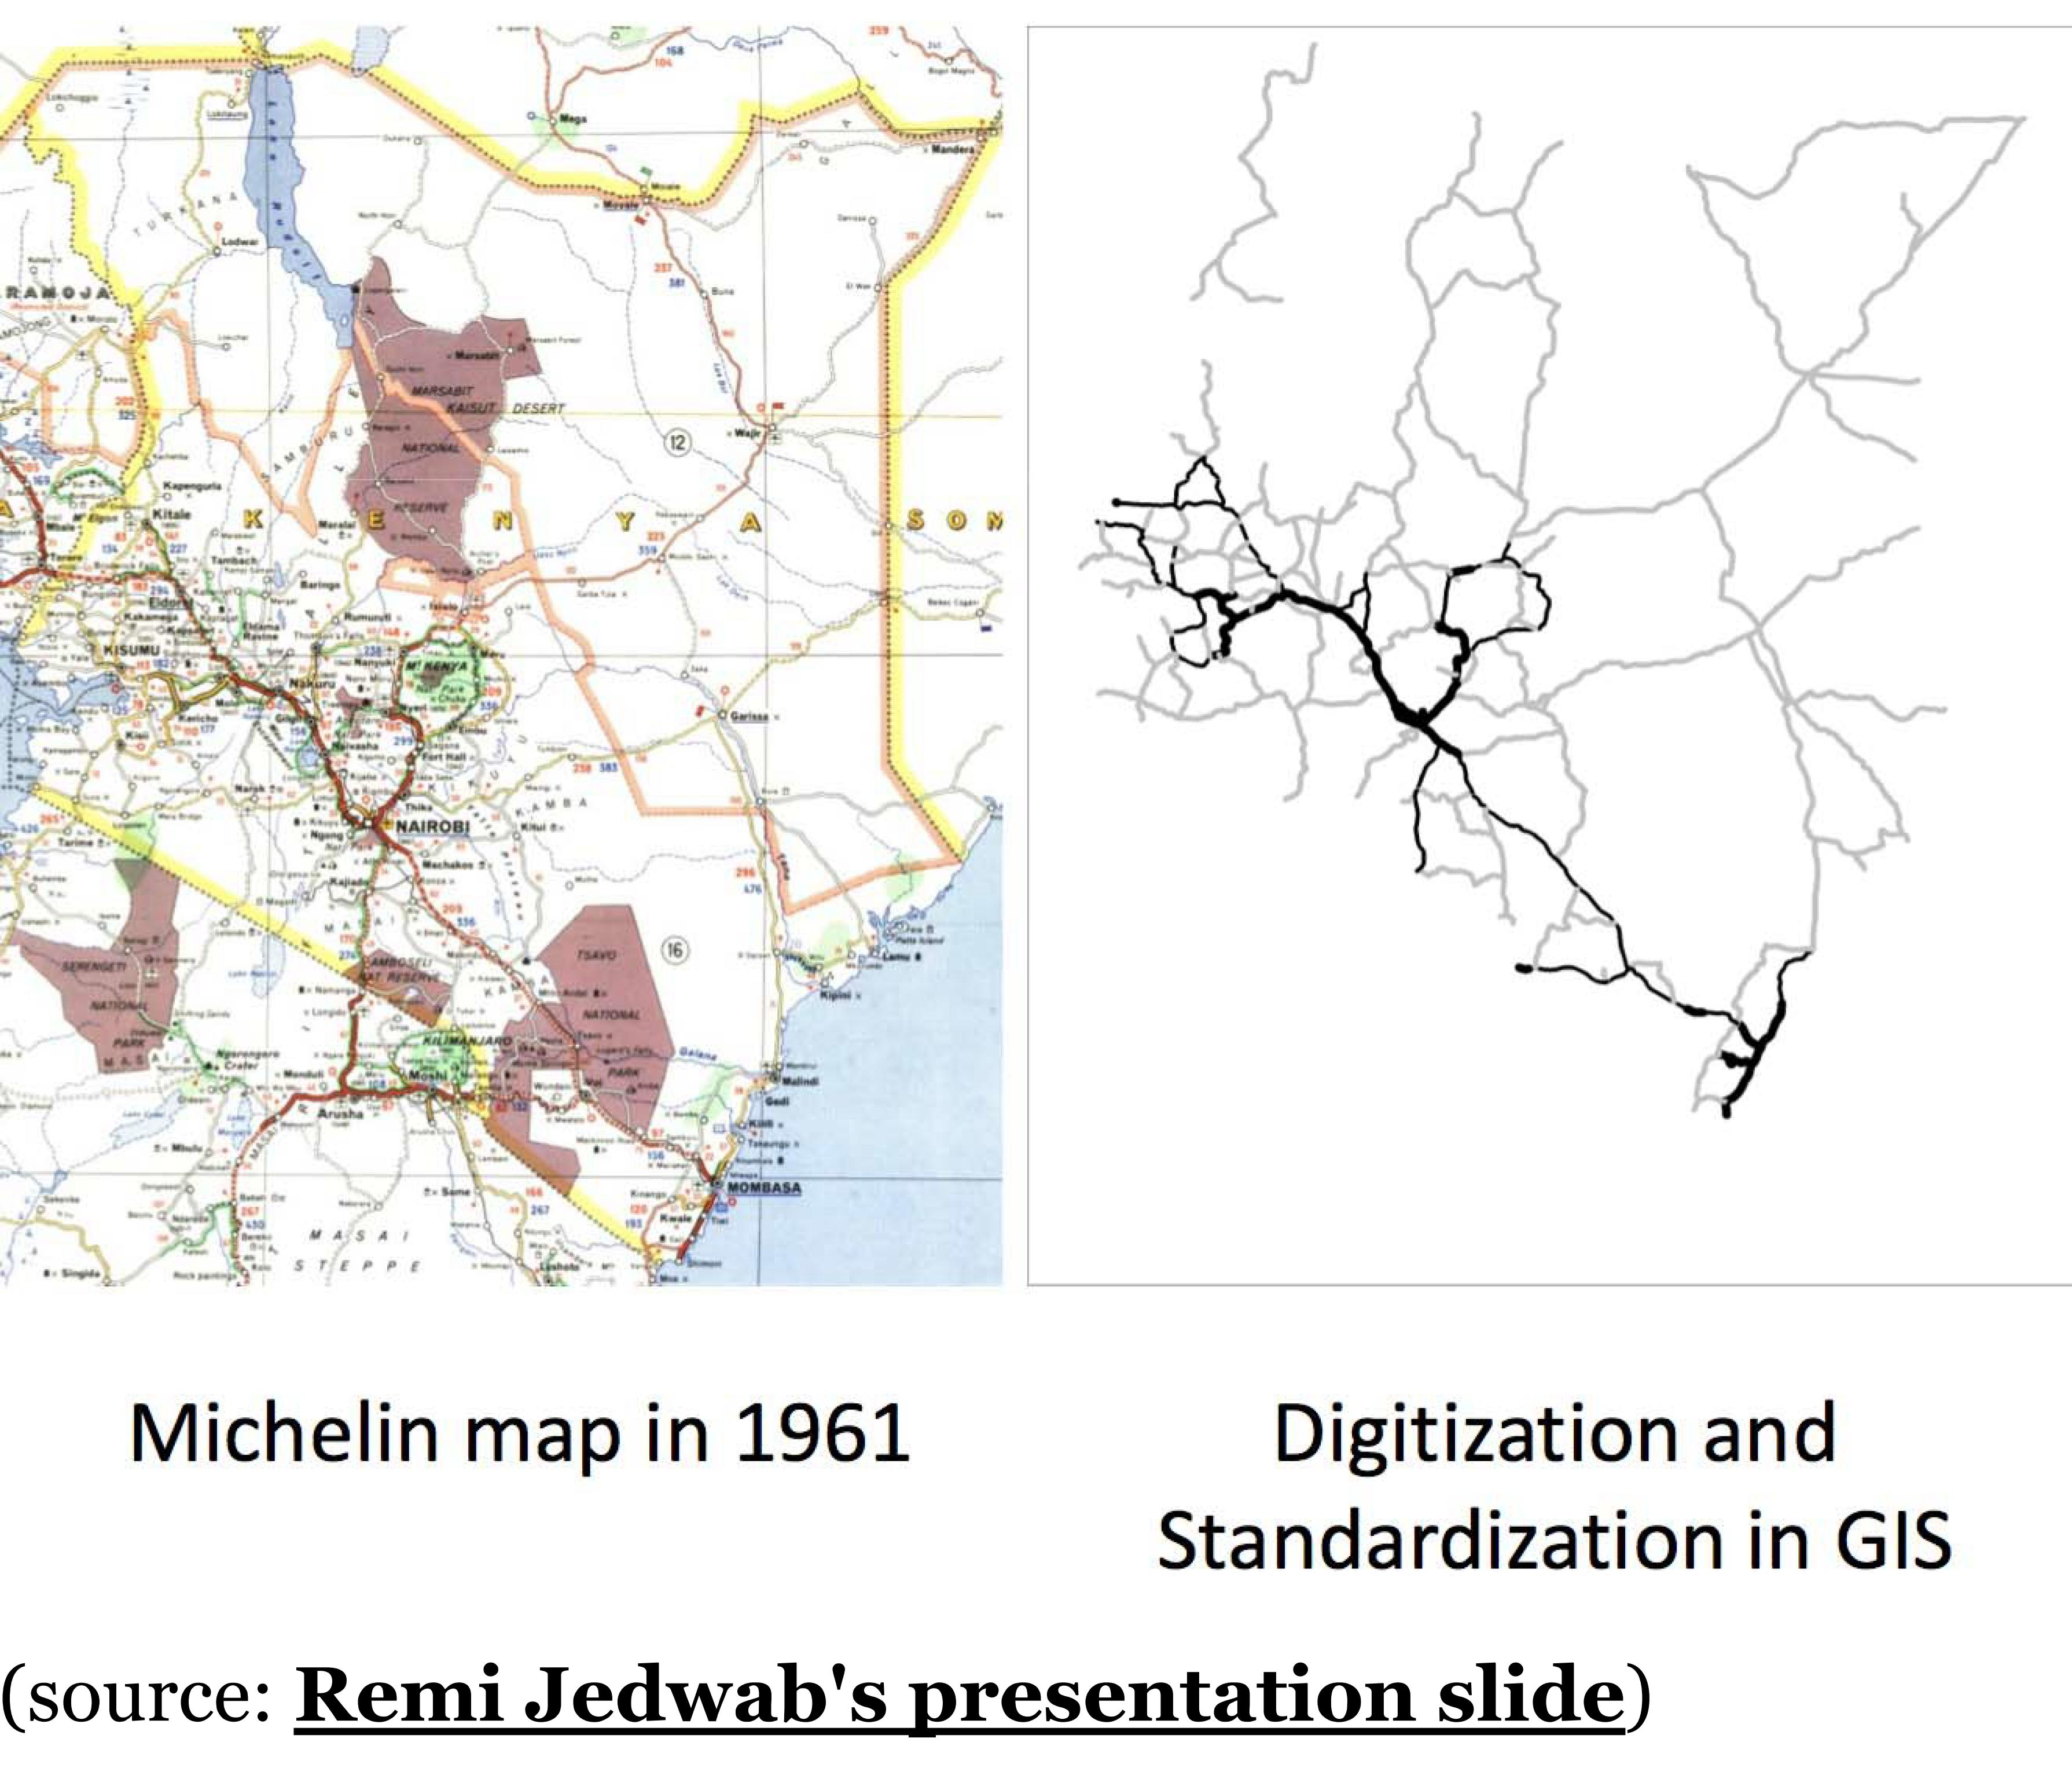
\includegraphics[width=.85\textwidth]{figure/kenya_road_f1.jpg}
	
% \end{frame}



% \begin{frame}{Make Research Feasible}{Example: Scanned Old Maps}
% 	\begin{itemize}
% 		\item They find strong evidence of ethnic favoritism
% 		\vspace{0.2cm}
% 		\item Districts that share the ethnicity of the president:  
% 		\begin{itemize}
% 			\vspace{0.2cm}
% 			\item Receive twice as much expenditure on roads 
% 			\vspace{0.2cm}
% 			\item Have five times the length of paved roads built
% 			\vspace{0.2cm}
% 			\item This favoritism disappears during periods of democracy
% 		\end{itemize}
% 	\end{itemize}
% \end{frame}


% =========================================================
% 修改後的 "Why GIS for Economists?" 投影片段落
% 主要修改：
%   1. 在 Why GIS 概覽頁新增第三個原因（大數據與新型資料來源）
%   2. 在衛星影像例子後新增一頁「更多衛星影像應用」
%   3. 在舊地圖例子後新增「其他新型地理資料來源」頁
%   4. 補充說明 Spatial RDD 的核心邏輯頁
% =========================================================


% ---------------------------------------------------------
% [修改] Frame 1：Why GIS for Economists? (概覽)
%   - 新增第三個原因：新型資料來源與大數據
% ---------------------------------------------------------
\begin{frame}{Why GIS for Economists?}{}
\begin{itemize}
	\item The use of geographic information system (GIS) has
	increasingly been popular among economists
	\vspace{0.2cm}
	\item There are at least three reasons for this popularity
	\vspace{0.2cm}
	\item[1] GIS allows economists to observe the previously unobserved
	and makes research feasible
	\vspace{0.2cm}
	\begin{itemize}
		\item Satellite images
		\vspace{0.2cm}
		\item Scanned old maps
		\vspace{0.2cm}
	\end{itemize}
	\item[2] GIS helps economists identify causal impacts in a more credible way than previously possible
	\begin{itemize}
		\vspace{0.2cm}
		\item Distance or Elevation
		\vspace{0.2cm}
		\item Geographic boundaries
	\end{itemize}
	\vspace{0.2cm}
	\item[3] GIS enables economists to combine large-scale administrative or commercial data with spatial information
	\begin{itemize}
		\vspace{0.2cm}
		\item Mobile phone data, credit card transactions, GPS tracking
	\end{itemize}
\end{itemize}
\end{frame}


% ---------------------------------------------------------
% [保留原文] Frame 2：Make Research Feasible - Satellite Images
% ---------------------------------------------------------
\begin{frame}{Make Research Feasible}{Example: Satellite Images}
J. Vernon Henderson, Adam Storeygard, and David N. Weil (2012), ``\textbf{Measuring Economic Growth from Outer Space}", AER
\begin{itemize}
\vspace{0.2cm}
\item They develop a statistical framework to use satellite data on night lights to estimate GDP growth
\vspace{0.2cm}
\begin{itemize}
\item Their estimates are quite close to official growth data
\vspace{0.2cm}
\end{itemize}
\item Using night lights data, empirical analyses of growth need no longer use countries as the unit of analysis
\vspace{0.2cm}
\begin{itemize}
\item Measure growth for sub- and supranational regions
\end{itemize}
\end{itemize}
\end{frame}


% ---------------------------------------------------------
% [保留原文] Frame 3：圖片 - World
% ---------------------------------------------------------
\begin{frame}{Satellite Images}{World}
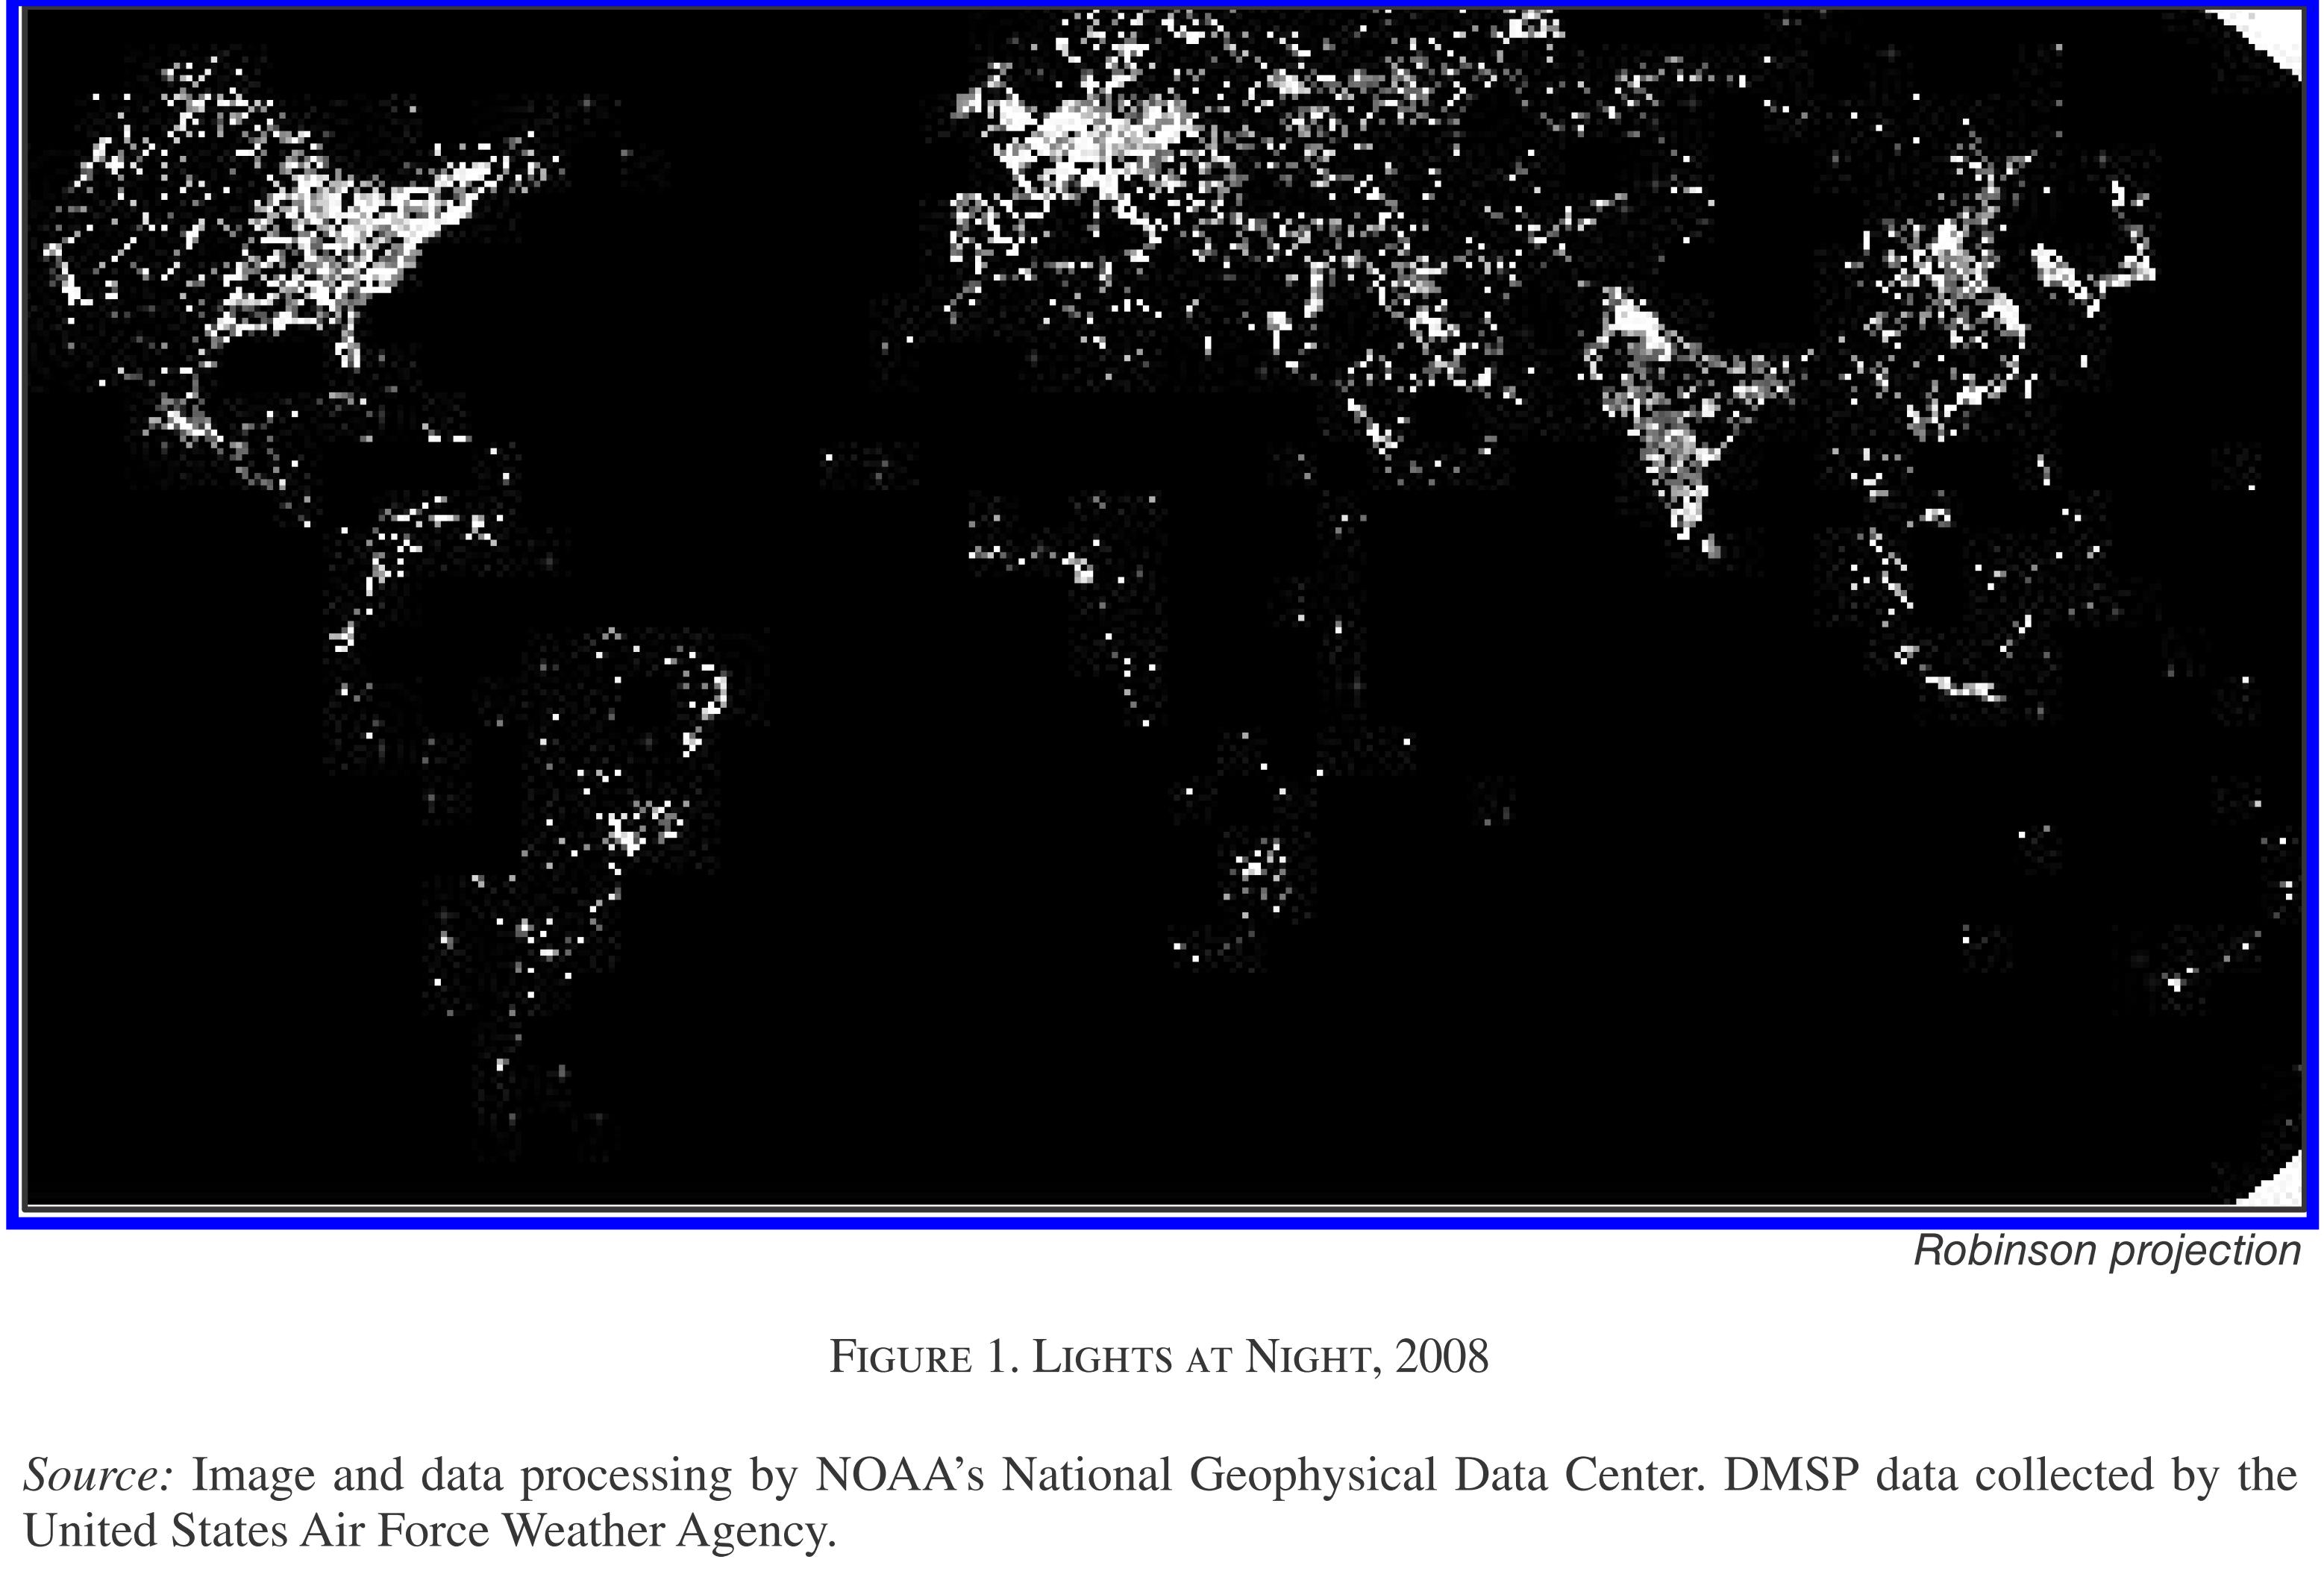
\includegraphics[width=0.9\textwidth]{figure/measure_g_f1.jpg}
\end{frame}


% ---------------------------------------------------------
% [保留原文] Frame 4：圖片 - Long-Run Growth in Korea
% ---------------------------------------------------------
\begin{frame}{Satellite Images}{Long-Run Growth in Korea}
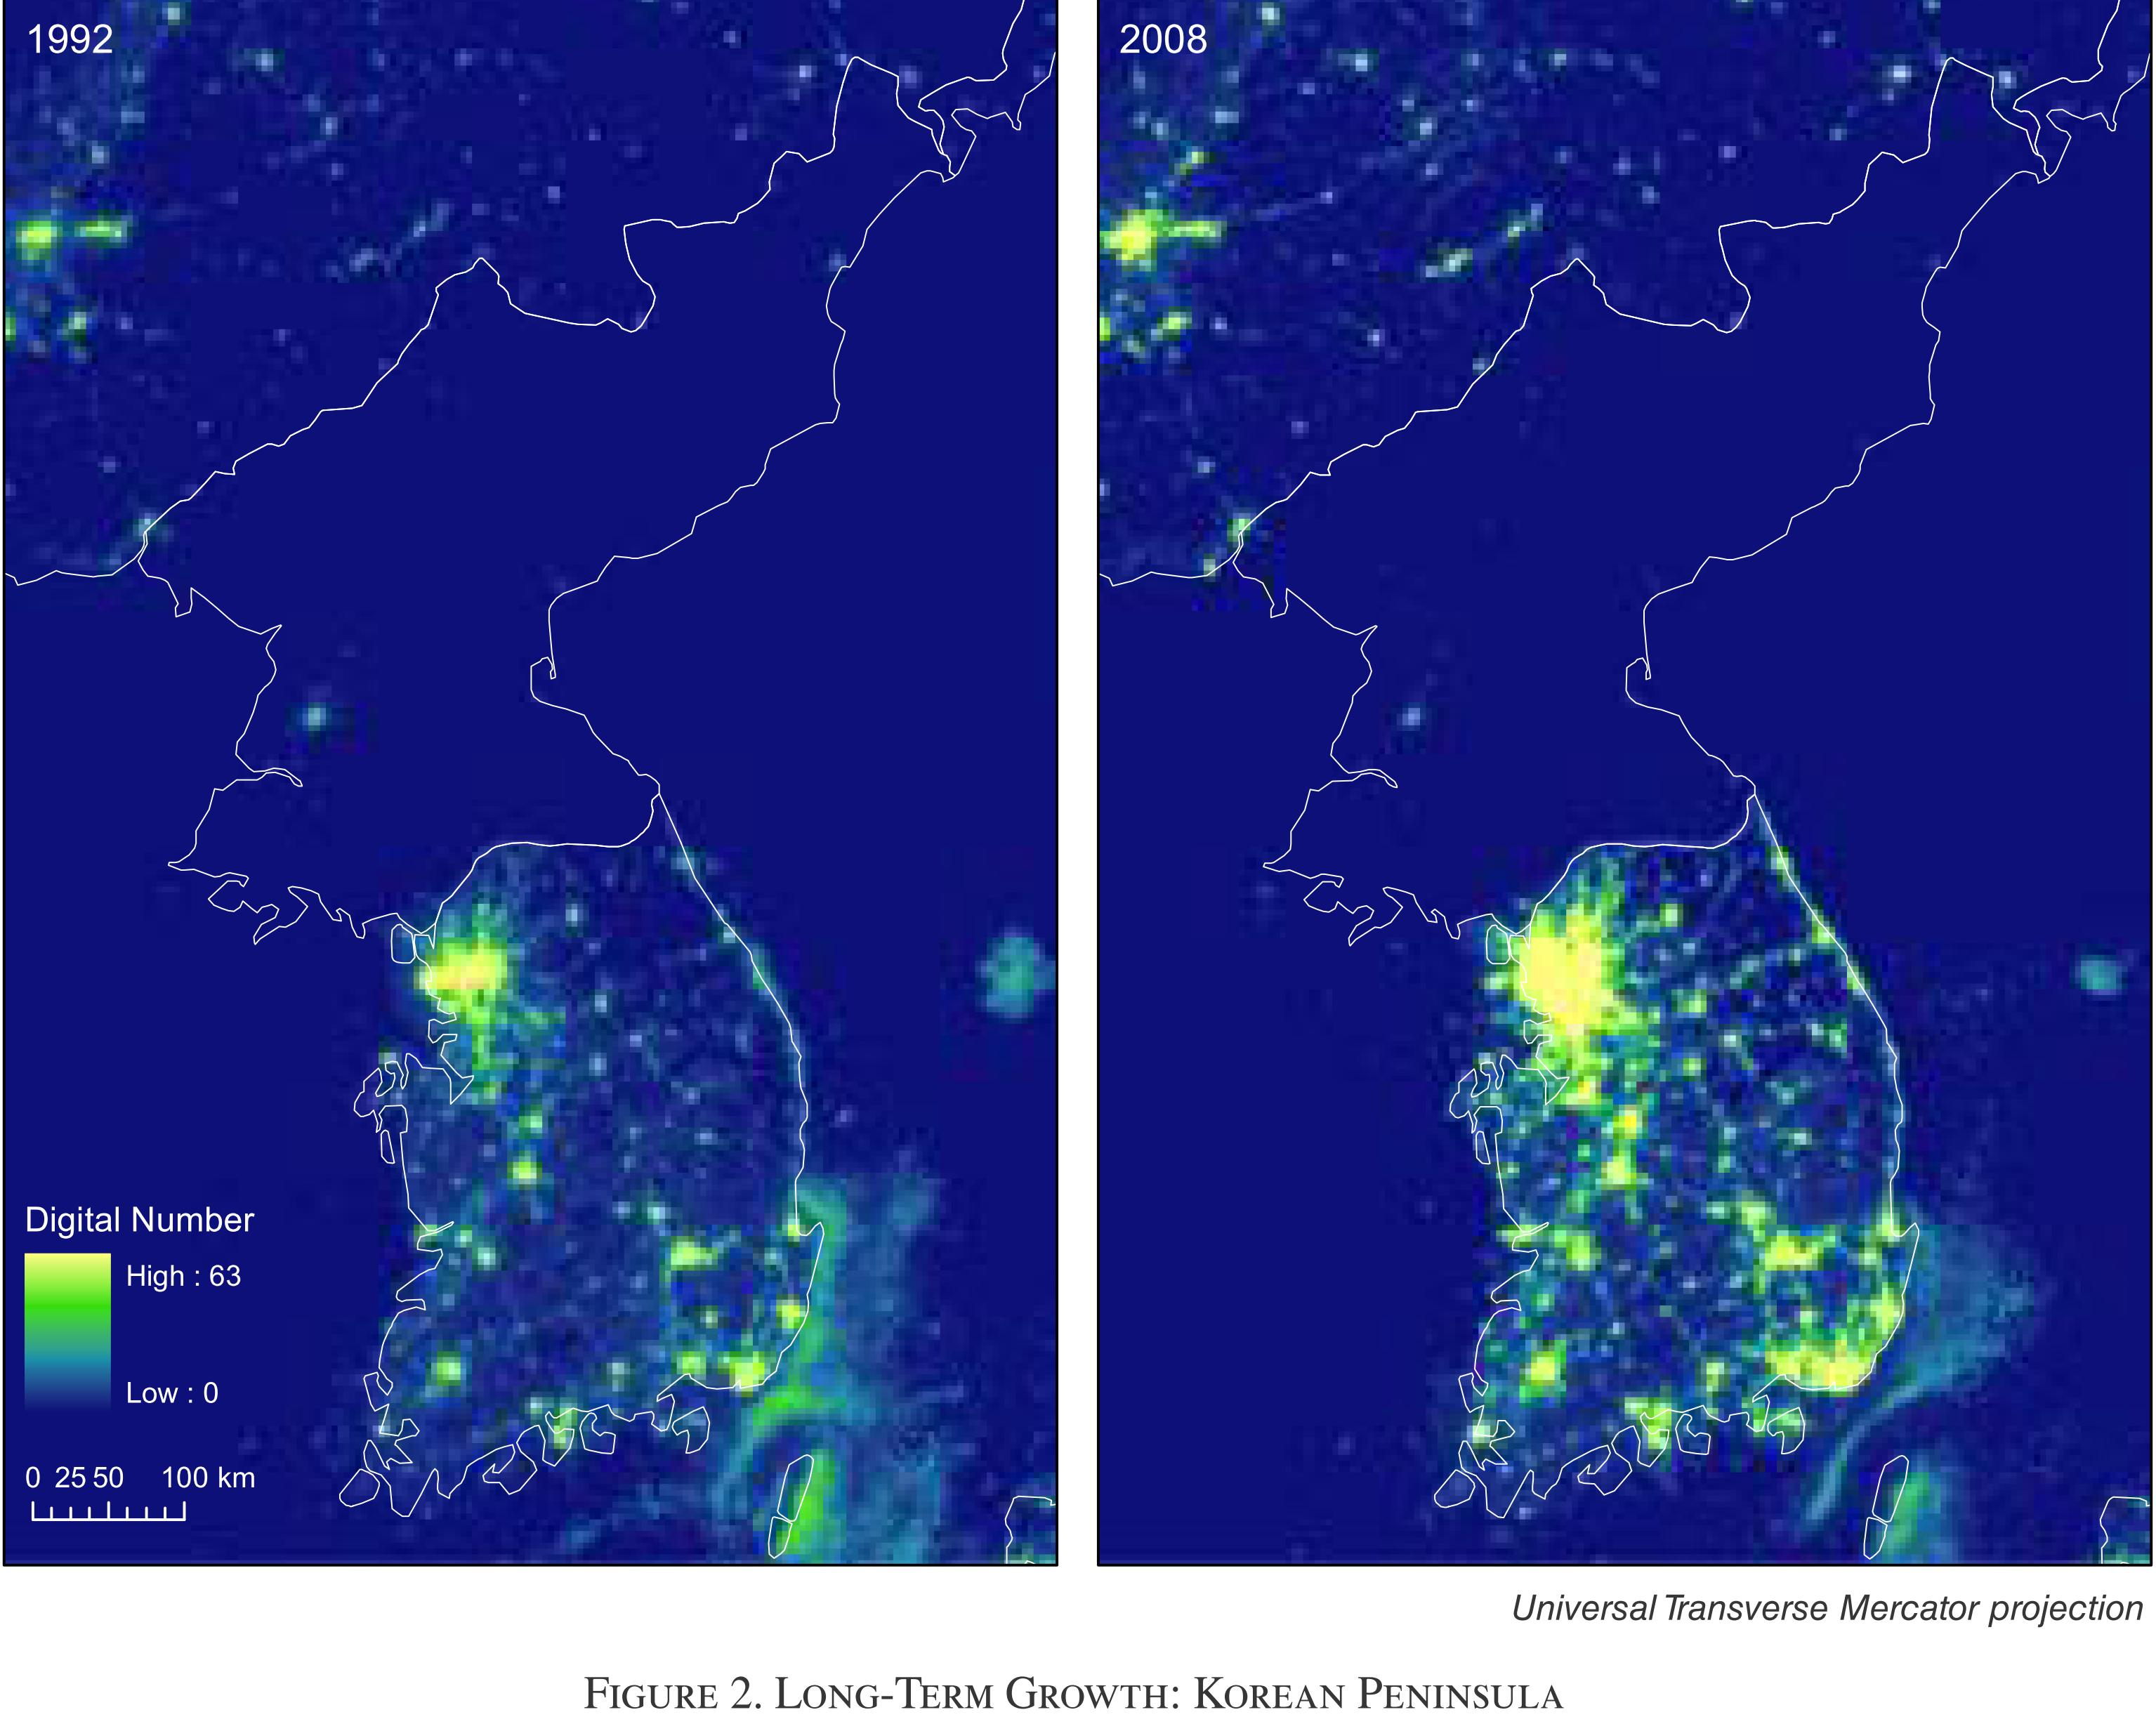
\includegraphics[width=0.9\textwidth]{figure/measure_g_f2.jpg}
\end{frame}


% ---------------------------------------------------------
% [新增] Frame 5：衛星影像的更多應用
%   - 補充 Donaldson & Storeygard (2016) 的文獻回顧角度
%   - 補充 conflict/poverty 等應用面向
% ---------------------------------------------------------
% ---------------------------------------------------------
% [修改] 原本一頁拆成兩頁
% ---------------------------------------------------------

% 頁一：夜間燈光的延伸應用
\begin{frame}{Satellite Images}{More Applications of Night Lights}
\begin{itemize}
    \item Night lights data have been applied in many contexts beyond GDP measurement
    \vspace{0.2cm}
    \begin{itemize}
        \item \textbf{Conflict and violence}: measure economic activity in war zones 
        where official statistics are unavailable
        \vspace{0.2cm}
        \item \textbf{Poverty mapping}: identify subnational poverty hotspots 
        in developing countries
        \vspace{0.2cm}
        \item \textbf{Urbanization}: track city growth and spatial expansion over time
    \end{itemize}
    \vspace{0.2cm}
    \item Two main data sources for night lights:
    \vspace{0.2cm}
    \begin{itemize}
        \item \textbf{DMSP-OLS} (1992--2013): 
        \href{https://eogdata.mines.edu/products/dmsp/}{\texttt{eogdata.mines.edu}}
        \vspace{0.2cm}
        \item \textbf{VIIRS DNB} (2012--present): 
        \href{https://eogdata.mines.edu/products/vnl/}{\texttt{eogdata.mines.edu/products/vnl}}
        \vspace{0.2cm}
        \item \textbf{NASA Black Marble} (VIIRS, high-res): 
        \href{https://blackmarble.gsfc.nasa.gov}{\texttt{earthdata.nasa.gov}}
    \end{itemize}
\end{itemize}
\end{frame}


% 頁二：NDVI
\begin{frame}{Other Satellite Data}{Vegetation Index (NDVI)}
\begin{itemize}
    \item \textbf{What it measures}: the ``greenness'' of land surface,
    reflecting vegetation health and density
    \vspace{0.2cm}
    \begin{itemize}
        \item $NDVI = \frac{NIR - Red}{NIR + Red}$, ranging from $-1$ to $+1$
        \vspace{0.1cm}
        \item Higher values $\Rightarrow$ denser, healthier vegetation
        \vspace{0.1cm}
        \item Negative values $\Rightarrow$ water bodies
    \end{itemize}
    \vspace{0.2cm}
    \item \textbf{Data}: NASA MODIS (250m--1km, 16-day or monthly)
    \vspace{0.2cm}
    \item \textbf{Applications in economics}:
    \vspace{0.1cm}
    \begin{itemize}
        \item Proxy for \textbf{agricultural productivity} and crop yields
        \vspace{0.1cm}
        \item Proxy for \textbf{rainfall} in areas with sparse weather stations
        \vspace{0.1cm}
        \item Instrument for \textbf{income shocks} in conflict and migration research
    \end{itemize}
    \vspace{0.2cm}
    \item \textbf{Source}: 
    \href{https://modis.gsfc.nasa.gov/data/dataprod/mod13.php}{modis.gsfc.nasa.gov}
\end{itemize}
\end{frame}


% 頁三：LST
\begin{frame}{Other Satellite Data}{Land Surface Temperature (LST)}
\begin{itemize}
    \item \textbf{What it measures}: temperature of the Earth's surface 
    itself (not air temperature)
    \vspace{0.2cm}
    \begin{itemize}
        \item Derived from thermal infrared radiation emitted by the surface
        \vspace{0.1cm}
        \item Surface temperature can differ substantially from 
        air temperature (e.g., asphalt on a hot day)
    \end{itemize}
    \vspace{0.2cm}
    \item \textbf{Data}: NASA MODIS MOD11 (1km, daily or 8-day composites)
    \vspace{0.2cm}
    \item \textbf{Advantage over weather stations}: 
    globally uniform coverage, no interpolation needed
    \vspace{0.2cm}
    \item \textbf{Applications in economics}:
    \vspace{0.1cm}
    \begin{itemize}
        \item \textbf{Urban heat islands}: link green space and 
        land use to housing prices
        \vspace{0.1cm}
        \item \textbf{Labor productivity}: estimate causal effect 
        of heat on wages and output
        \vspace{0.1cm}
        \item \textbf{Energy demand}: high temperatures raise 
        cooling demand and electricity consumption
    \end{itemize}
    \vspace{0.2cm}
    \item \textbf{Source}: 
    \href{https://modis.gsfc.nasa.gov/data/dataprod/}{modis.gsfc.nasa.gov}
\end{itemize}
\end{frame}


% 頁四：AOD
\begin{frame}{Other Satellite Data}{Aerosol Optical Depth (AOD)}
\begin{itemize}
    \item \textbf{What it measures}: how much sunlight is blocked 
    by suspended particles across the entire atmospheric column
    \vspace{0.2cm}
    \begin{itemize}
        \item AOD $= 0$: clean, transparent atmosphere
        \vspace{0.1cm}
        \item AOD $= 1$: heavy particulate loading (smoke, dust, pollution)
    \end{itemize}
    \vspace{0.2cm}
    \item \textbf{Data}: NASA MODIS MOD04 (3km--10km, daily)
    \vspace{0.2cm}
    \item \textbf{Why use AOD instead of PM2.5?}
    \vspace{0.1cm}
    \begin{itemize}
        \item Ground PM2.5 monitors are sparse, especially 
        in developing countries
        \vspace{0.1cm}
        \item AOD provides global, uniform coverage since 2000
        \vspace{0.1cm}
        \item Caveat: AOD measures the full atmospheric column; 
        conversion to ground-level PM2.5 requires additional modeling
    \end{itemize}
    \vspace{0.2cm}
    \item \textbf{Applications in economics}:
    \vspace{0.1cm}
    \begin{itemize}
        \item Pollution effects on \textbf{health, cognition, and productivity}
        \vspace{0.1cm}
        \item Evaluation of \textbf{environmental regulations}
    \end{itemize}
    \vspace{0.1cm}
    \item \textbf{Source}: 
    \href{https://modis.gsfc.nasa.gov/data/dataprod/}{modis.gsfc.nasa.gov} 
    $\cdot$ All products free at 
    \href{https://earthdata.nasa.gov}{earthdata.nasa.gov}
\end{itemize}
\end{frame}

% ---------------------------------------------------------
% [保留原文] Frame 6：Make Research Feasible - Scanned Old Maps (問題)
% ---------------------------------------------------------
%districts that share the ethnicity of the president receive twice as much expenditure on roads and have five times the length of paved roads built
\begin{frame}{Make Research Feasible}{Example: Scanned Old Maps}
	Robin Burgess, Remi Jedwab, Edward Miguel,
	Ameet Morjaria, and Gerard Padr\'o i Miquel (2015), ``\textbf{The Value of Democracy:
		Evidence from Road Building in Kenya}", AER
	\begin{itemize}
		\vspace{0.2cm}
		\item Did Kenyan presidents build more roads for their co-ethnics?
		\vspace{0.2cm}
		\begin{itemize}
			\item They digitalized the old maps to get the building of roads since the year of independence in Kenya (1961)
			\vspace{0.2cm}
			\item Track road network expansion over time
		\end{itemize}
	\end{itemize}
\end{frame}


% ---------------------------------------------------------
% [保留原文] Frame 7：圖片 - Kenya 1961
% ---------------------------------------------------------
\begin{frame}{Scanned Old Maps}{Map of Roads in Kenya in 1961}
	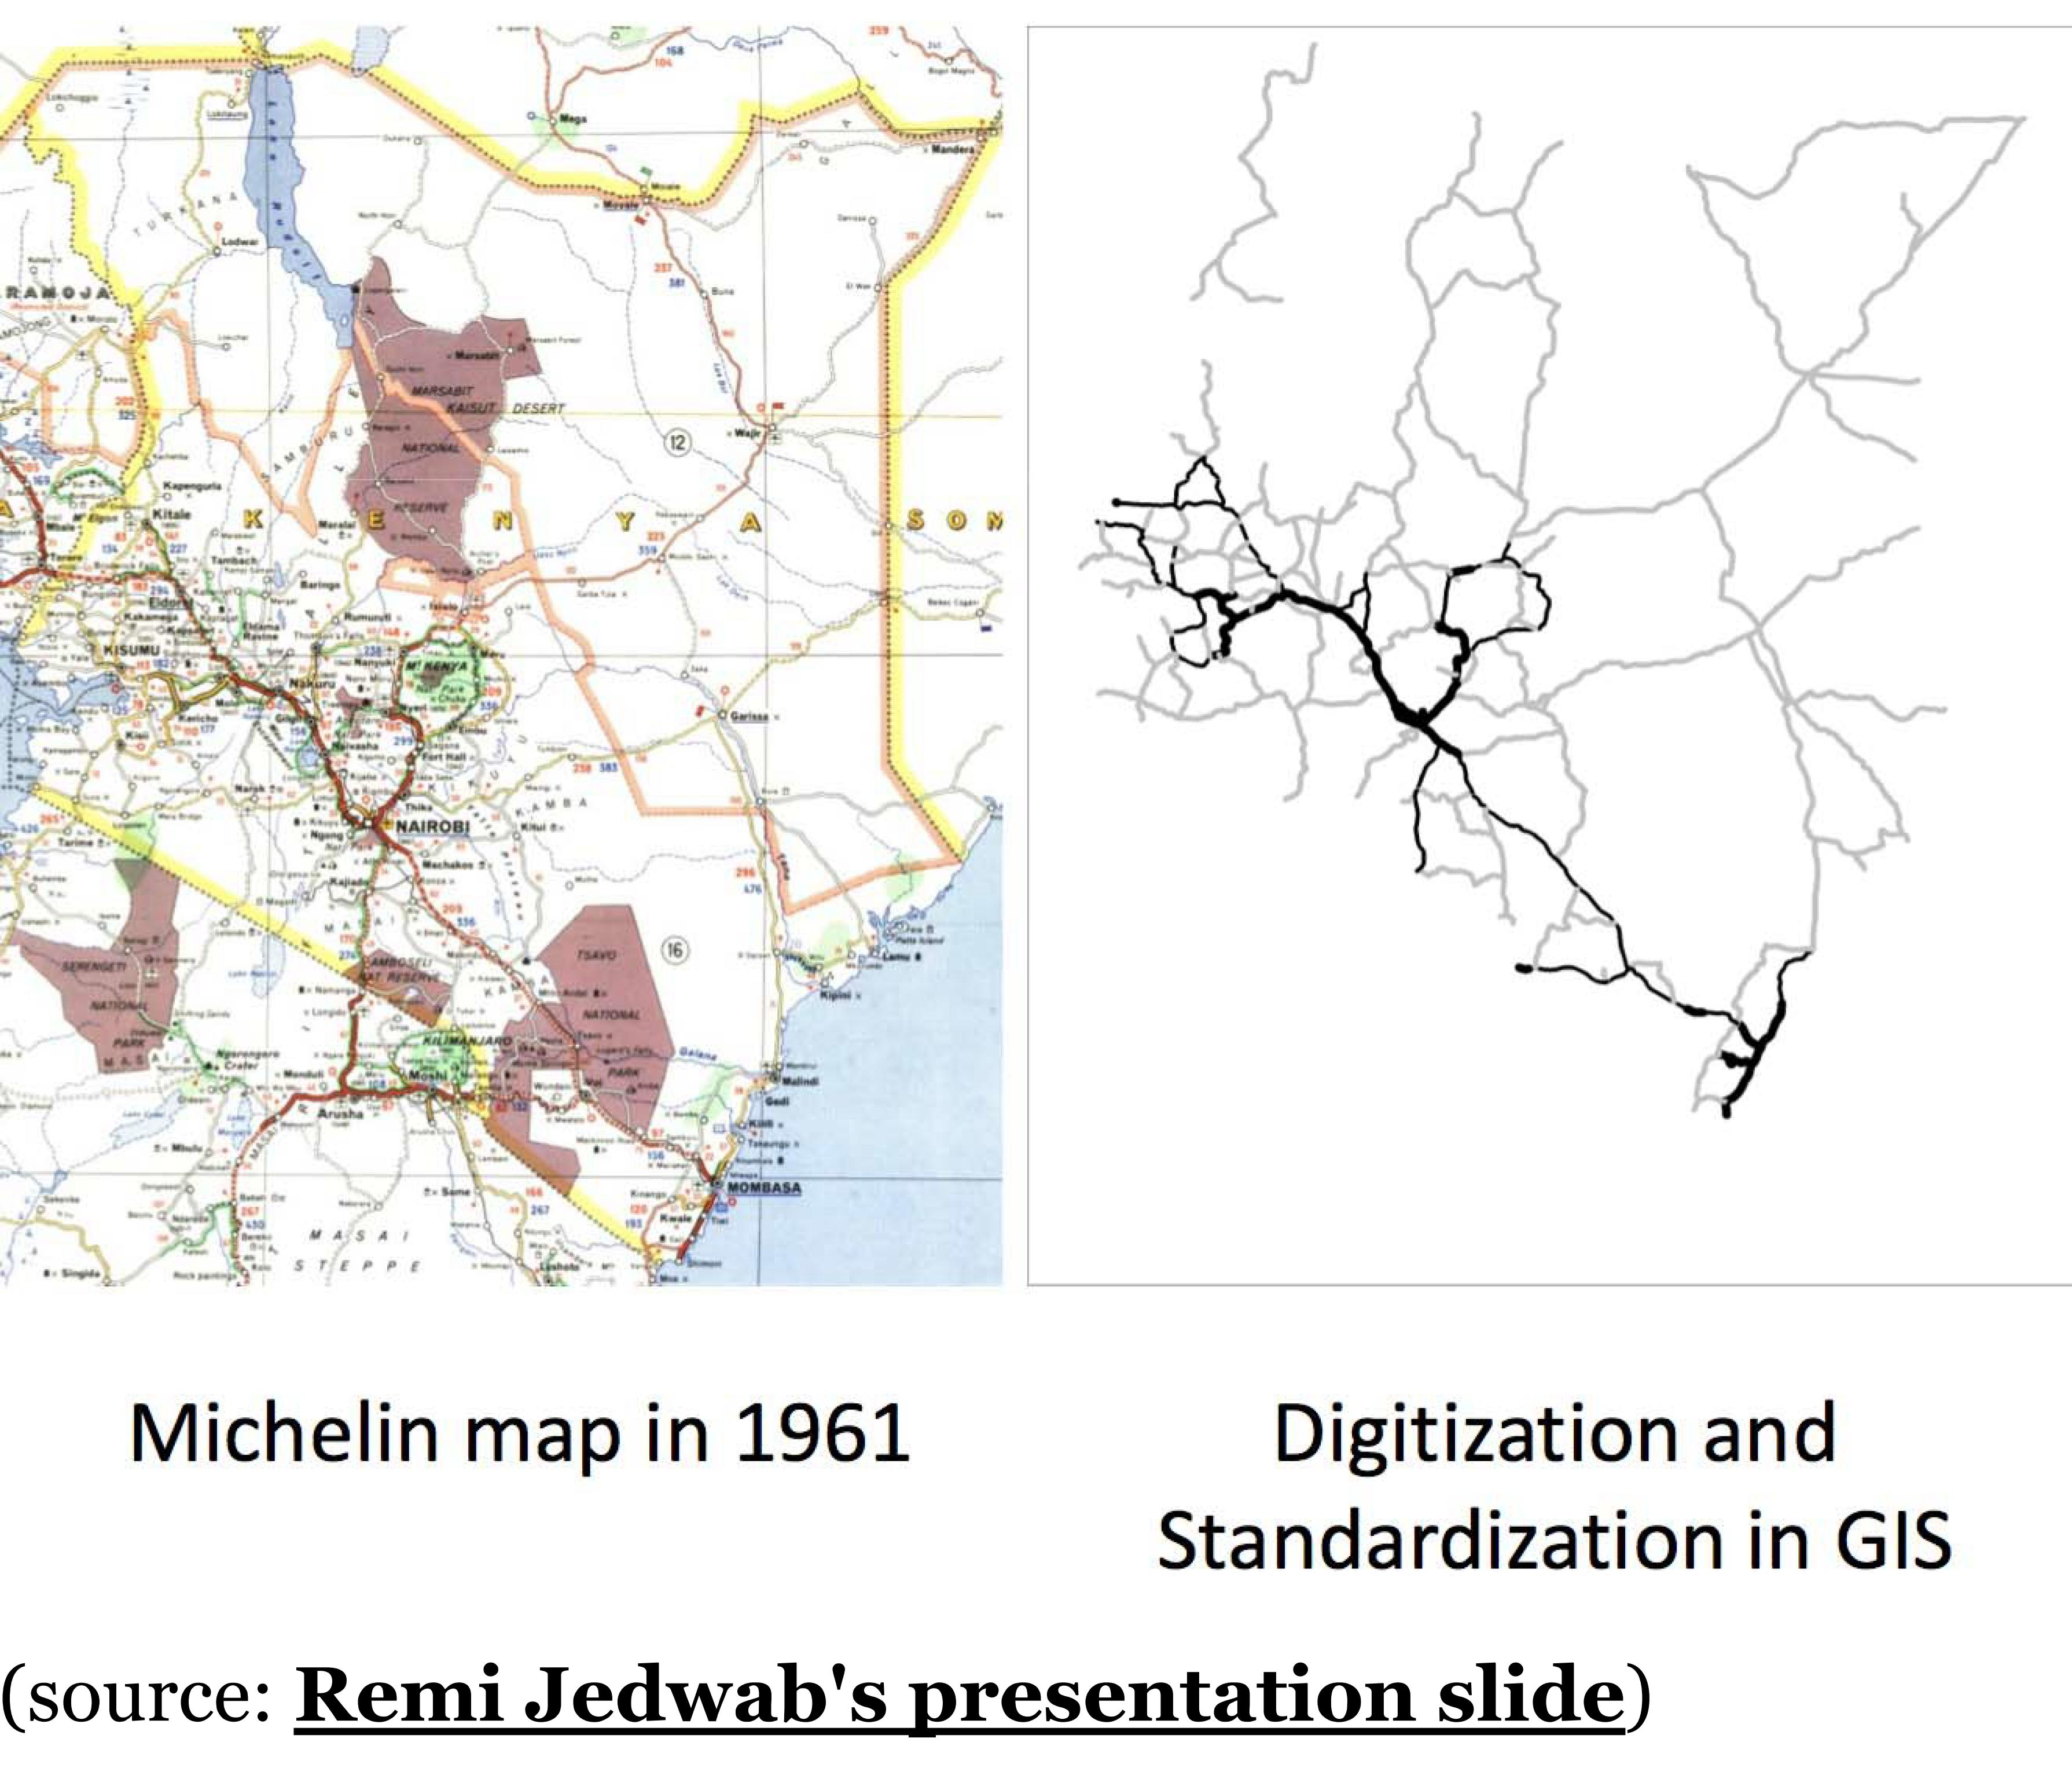
\includegraphics[width=.85\textwidth]{figure/kenya_road_f1.jpg}
\end{frame}


% ---------------------------------------------------------
% [保留原文] Frame 8：Make Research Feasible - Scanned Old Maps (結果)
% ---------------------------------------------------------
\begin{frame}{Make Research Feasible}{Example: Scanned Old Maps}
	\begin{itemize}
		\item They find strong evidence of ethnic favoritism
		\vspace{0.2cm}
		\item Districts that share the ethnicity of the president:
		\begin{itemize}
			\vspace{0.2cm}
			\item Receive twice as much expenditure on roads
			\vspace{0.2cm}
			\item Have five times the length of paved roads built
			\vspace{0.2cm}
			\item This favoritism disappears during periods of democracy
		\end{itemize}
	\end{itemize}
\end{frame}


% ---------------------------------------------------------
% [新增] Frame 9：其他新型地理資料來源
%   - 說明「新型資料來源」這個第三個原因的具體例子
% ---------------------------------------------------------
\begin{frame}{New Data Sources}{Beyond Maps and Satellites}
\begin{itemize}
	\item Recent advances in data collection have opened new frontiers for spatial economics
	\vspace{0.2cm}
	\item \textbf{Mobile phone / GPS data}
	\begin{itemize}
		\vspace{0.1cm}
		\item Track individual mobility patterns, commuting flows, and migration
		\vspace{0.1cm}
		\item Estimate local economic activity via foot traffic
	\end{itemize}
	\vspace{0.2cm}
	\item \textbf{Geotagged social media and text data}
	\begin{itemize}
		\vspace{0.1cm}
		\item Measure consumer sentiment, disaster response, or social interactions at the neighborhood level
	\end{itemize}
	\vspace{0.2cm}
	\item \textbf{Historical aerial photographs and colonial records}
	\begin{itemize}
		\vspace{0.1cm}
		\item Reconstruct pre-independence land use, property rights, and infrastructure
		\vspace{0.1cm}
		\item Similar to the Kenya road map digitization approach
	\end{itemize}
	\vspace{0.2cm}
	\item These data sources are often combined with GIS to link spatial and non-spatial information
\end{itemize}
\end{frame}


% ---------------------------------------------------------
% [新增] Frame 10：Spatial RDD 的核心識別邏輯補充
%   - 在原本 "identify causal impacts" 區塊之前，
%     補充說明為什麼地理邊界可以作為 RDD 的斷點
% ---------------------------------------------------------
\begin{frame}{Identify Causal Impacts}{Why Geography Helps}
\begin{itemize}
	\item A central challenge in economics: policies, treatments, and exposures are \textbf{not randomly assigned}
	\vspace{0.2cm}
	\item GIS provides tools to construct \textbf{credible comparison groups} using geographic variation:
	\vspace{0.2cm}
	\begin{itemize}
		\item \textbf{Distance} as an instrumental variable
        		\vspace{0.2cm}
		\begin{itemize}
			\item Distance to a trade hub, river, coast, or infrastructure node affects treatment but is plausibly exogenous
		\end{itemize}
		\vspace{0.2cm}
		\item \textbf{Elevation / terrain} as an instrumental variable
        		\vspace{0.2cm}
		\begin{itemize}
			\item Ruggedness or slope affects infrastructure rollout costs
		\end{itemize}
		\vspace{0.2cm}
		\item \textbf{Administrative boundaries} for Spatial RDD
		\begin{itemize}
			\item Policies often change sharply at borders
            		\vspace{0.2cm}
			\item Locations just inside vs.\ just outside a border are similar in all other respects
		\end{itemize}
	\end{itemize}
\end{itemize}
\end{frame}



\begin{frame}{Identify Causal Impacts}{Example: Distance}
	Nathan Nunn (2008), ``\textbf{The Long-term Effects of Africa's Slave Trades}", QJE
	
	\begin{itemize}
		\vspace{0.2cm}
		\item Can part of Africa's current underdevelopment be explained by its slave
		trades ?
		\vspace{0.2cm}
		\begin{itemize}
			\item More slave trades leads to lower growth in Africa  
			
			%He uses data from shipping records and historical documents reporting slave ethnicities to construct estimates of the number of slaves exported from each country during Africa's slave trades
			\vspace{0.2cm}
			\item  Since slave trades may be endogenous to the historical level of development
		\end{itemize}
		\vspace{0.2cm}
		\item IV for slave trade: 
		\begin{itemize}
			\vspace{0.2cm}
			\item Slave trade: the number of exported slaves from each country.
			\vspace{0.2cm}
			\item IV: distance to the nearest slave trade center in the Americas
		\end{itemize}
	\end{itemize}
\end{frame}

\begin{frame}{Use Distance as an IV}{}
	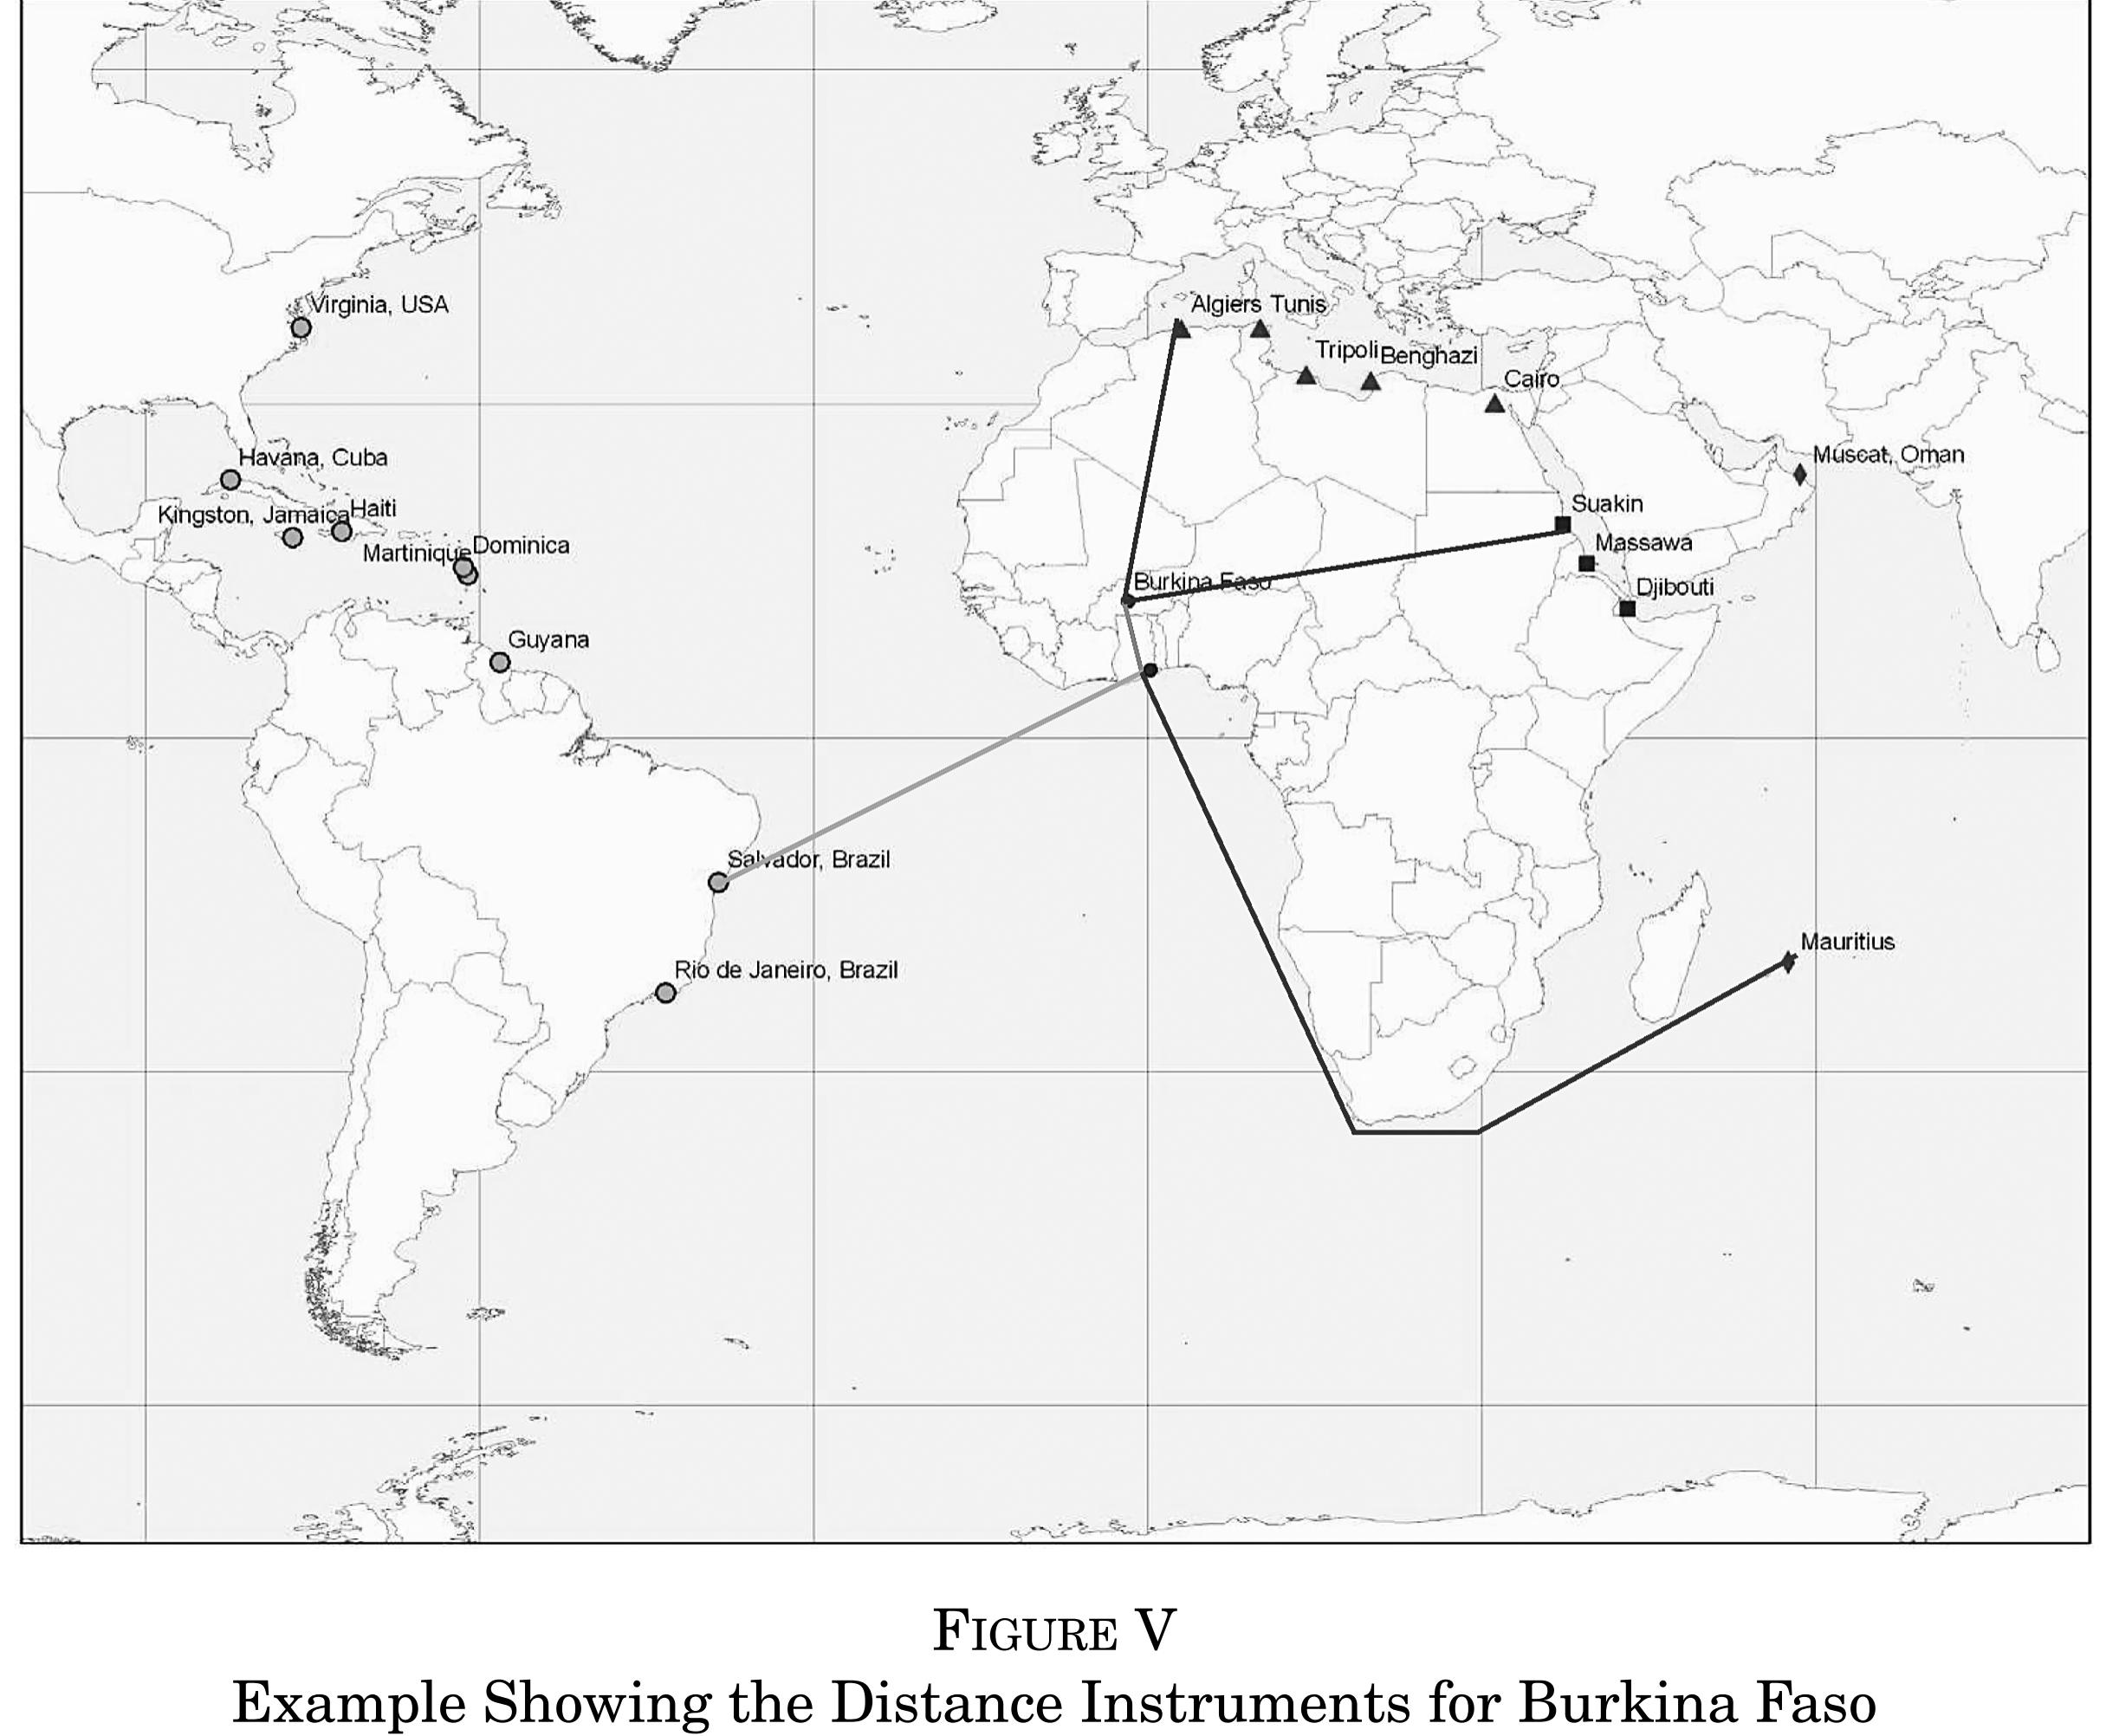
\includegraphics[width=.90\textwidth]{figure/slave_f5.jpg}
	
\end{frame}

\begin{frame}{Identify Causal Impacts}{Example: Distance}	
	\begin{itemize}
		\item Location of slave trade centers:
		\begin{itemize}
			\vspace{0.2cm}
			\item Determined by climate suitability of plantation crops/location of mines
			\vspace{0.2cm}
			\item Not affected by the distance to Africa
			\vspace{0.2cm}
			\item Distance to slave markets $\neq$ Distance to other economic opportunities
			\vspace{0.2cm}
		\end{itemize}
		\item The author finds that countries with more slaves exported are poorer today
	\end{itemize}
\end{frame}





\begin{frame}{Identify Causal Impacts}{Example: Land Slope}
    Taryn Dinkelman (2011), ``\textbf{The Effects of Rural 
    Electrification on Employment: New Evidence from South Africa}", AER
    \begin{itemize}
        \item This paper estimates the impact of electrification 
        on female labor supply
        \vspace{0.2cm}
        \item IV for electrification: mean land slope
        \vspace{0.2cm}
        \begin{itemize}
            \item Flat terrain $\Rightarrow$ cheaper to lay power lines 
            $\Rightarrow$ more likely to be electrified
            \vspace{0.2cm}
            \item Land slope is determined by geology, 
            not by economic conditions
        \end{itemize}
        \vspace{0.2cm}
        \item They find that electrification significantly raises 
        female employment by:
        \begin{itemize}
            \vspace{0.2cm}
            \item Releasing women from home production
            \vspace{0.2cm}
            \item Enabling microenterprises
        \end{itemize}
    \end{itemize}
\end{frame}



\begin{frame}{Use Elevation as an IV}{}
	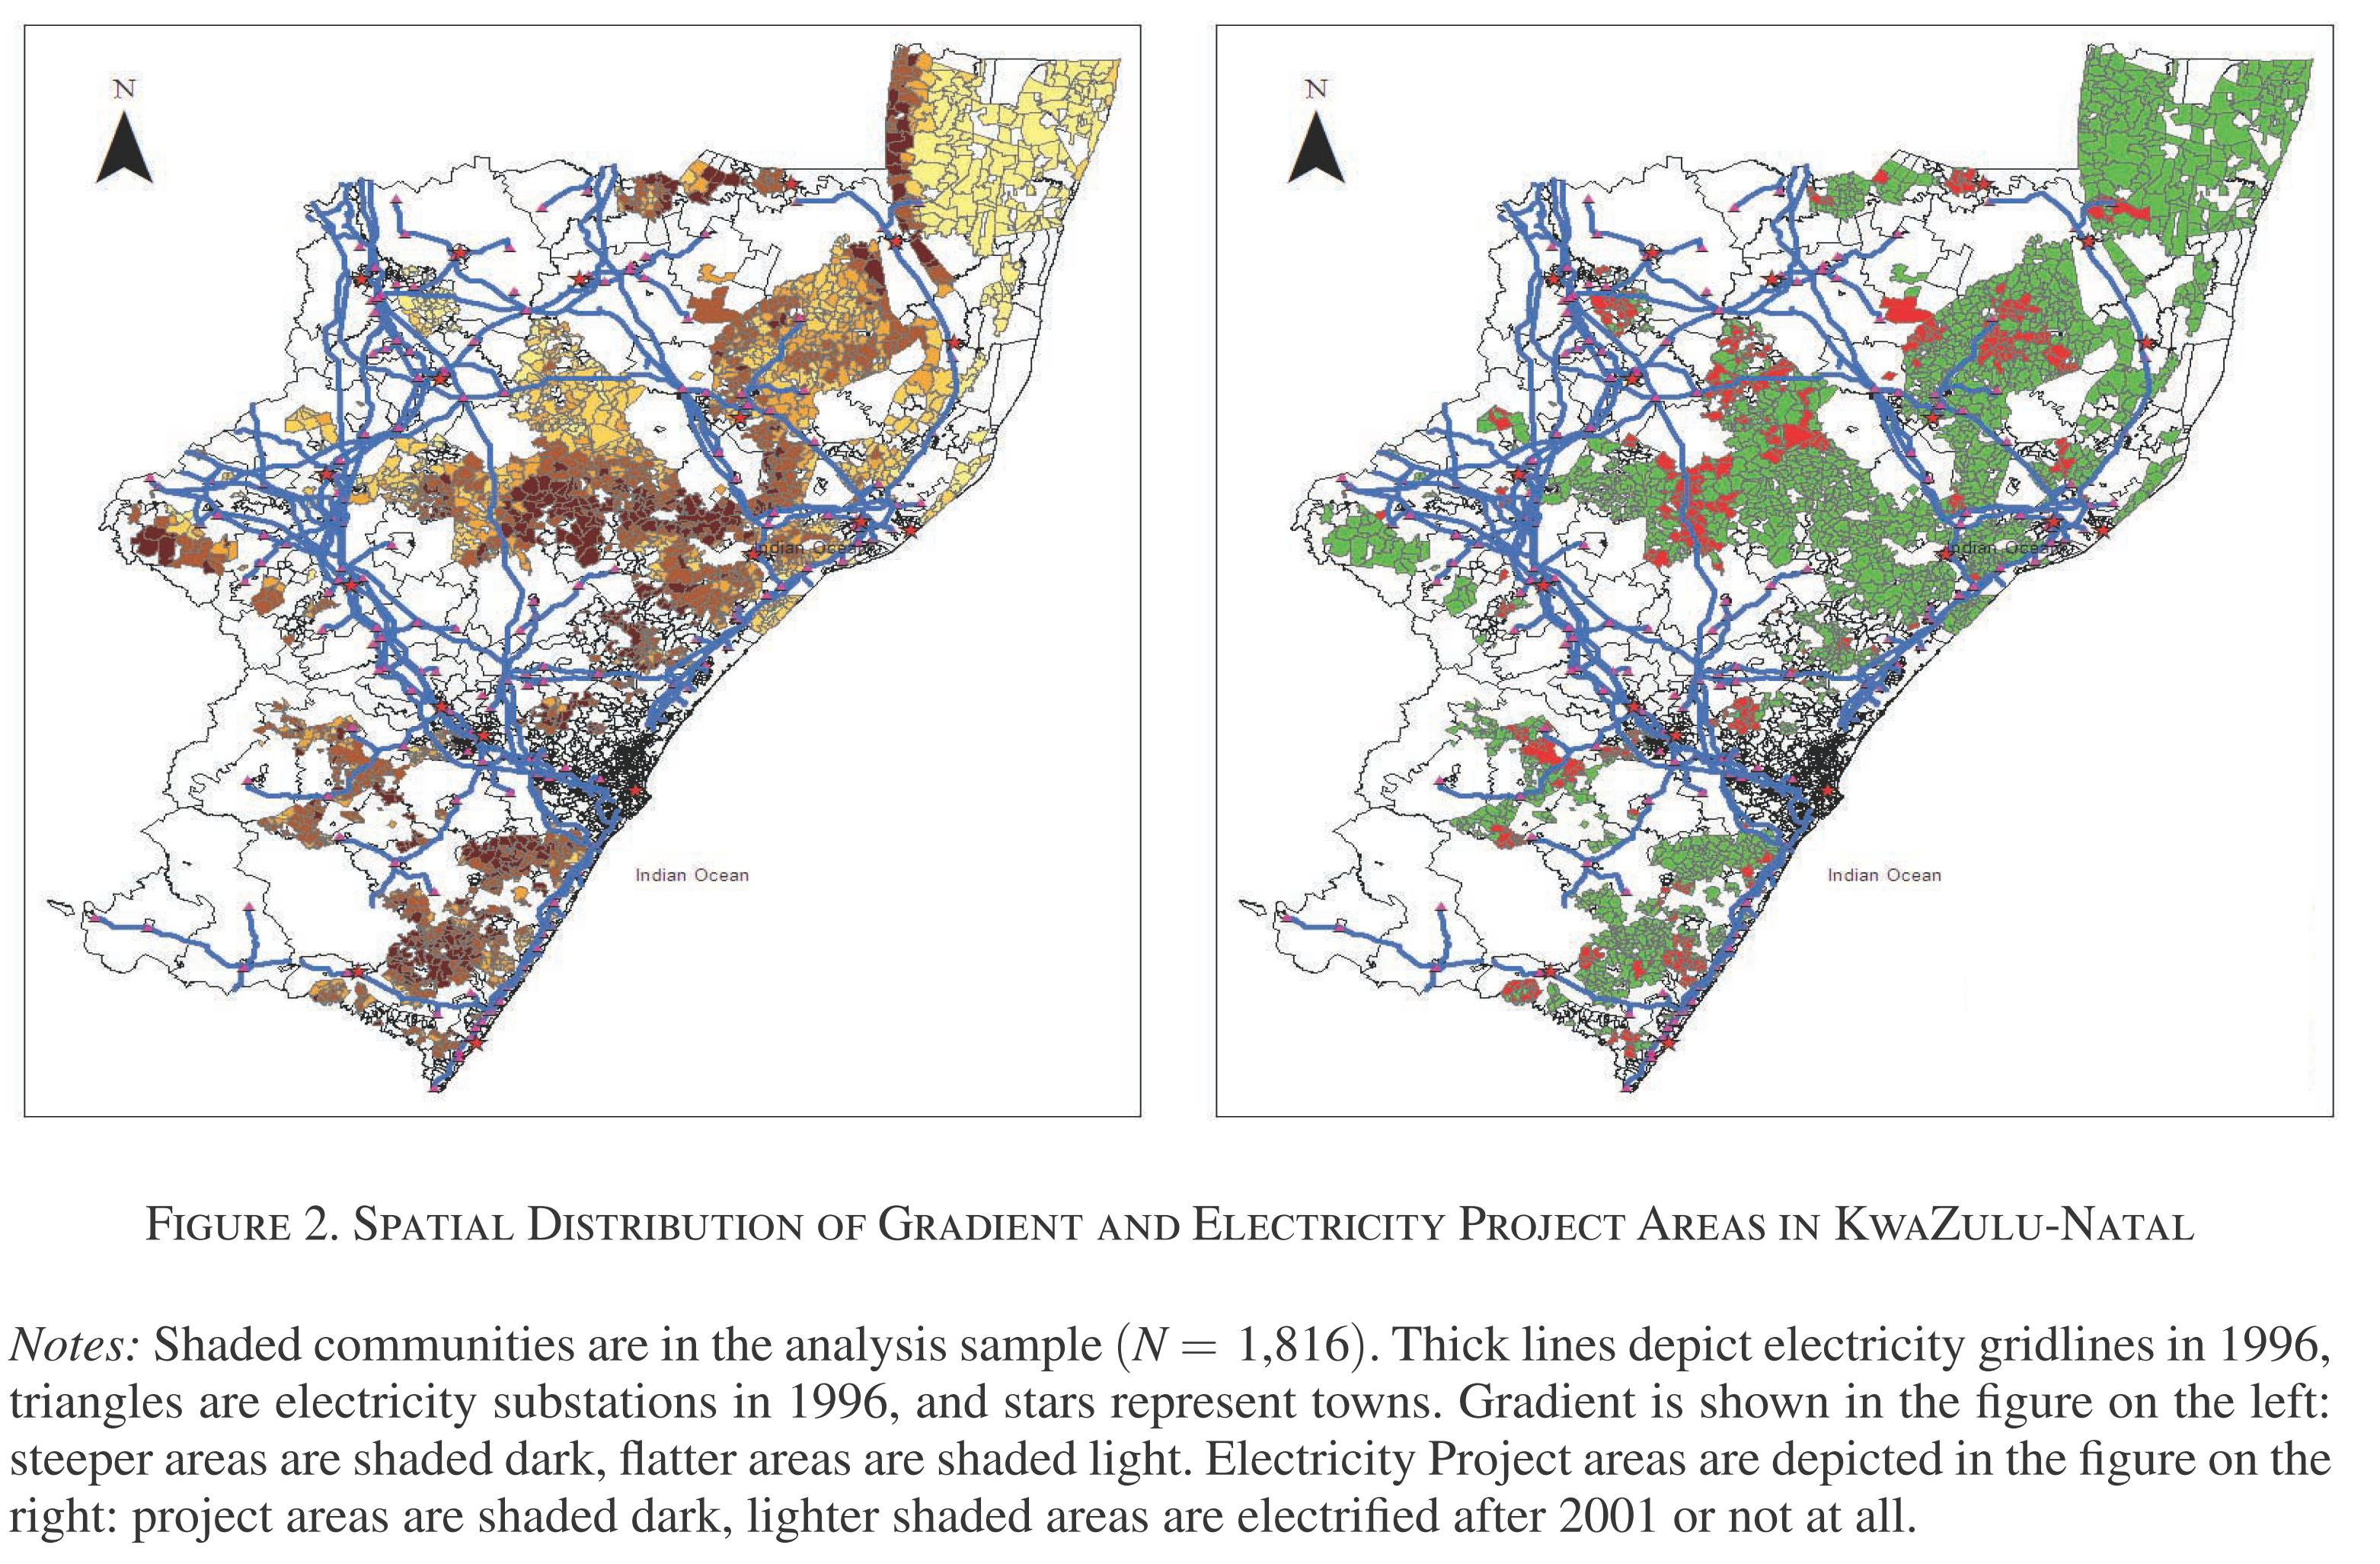
\includegraphics[width=.95\textwidth]{figure/electric_f2.jpg}
	
	\begin{itemize}
		\item Slope (lighter = flatter)
		\vspace{0.2cm}
		\item Electrification (red)
	\end{itemize}
\end{frame}



\begin{frame}{Identify Causal Impacts}{Example: Spatial Regression Discontinuity Design}
	Rafael Lalive (2008), ``\textbf{How do extended benefits affect unemployment duration?
		A regression discontinuity approach}", Journal of Econometrics
	\begin{itemize}
		\vspace{0.2cm}
		\item This paper examine the effect of extended benefits on unemployment duration using spatial RDD
		\vspace{0.2cm}
		\begin{itemize}
			\item Sharp discontinuities in treatment assignment at age 50 and at the border between eligible regions and control regions 
			\vspace{0.2cm}
			\item Extend the maximum duration of unemployment benefits from 30 weeks to 209 weeks
		\end{itemize}
		
	\end{itemize}
\end{frame}


\begin{frame}{Spatial Regression Discontinuity Design}{}
	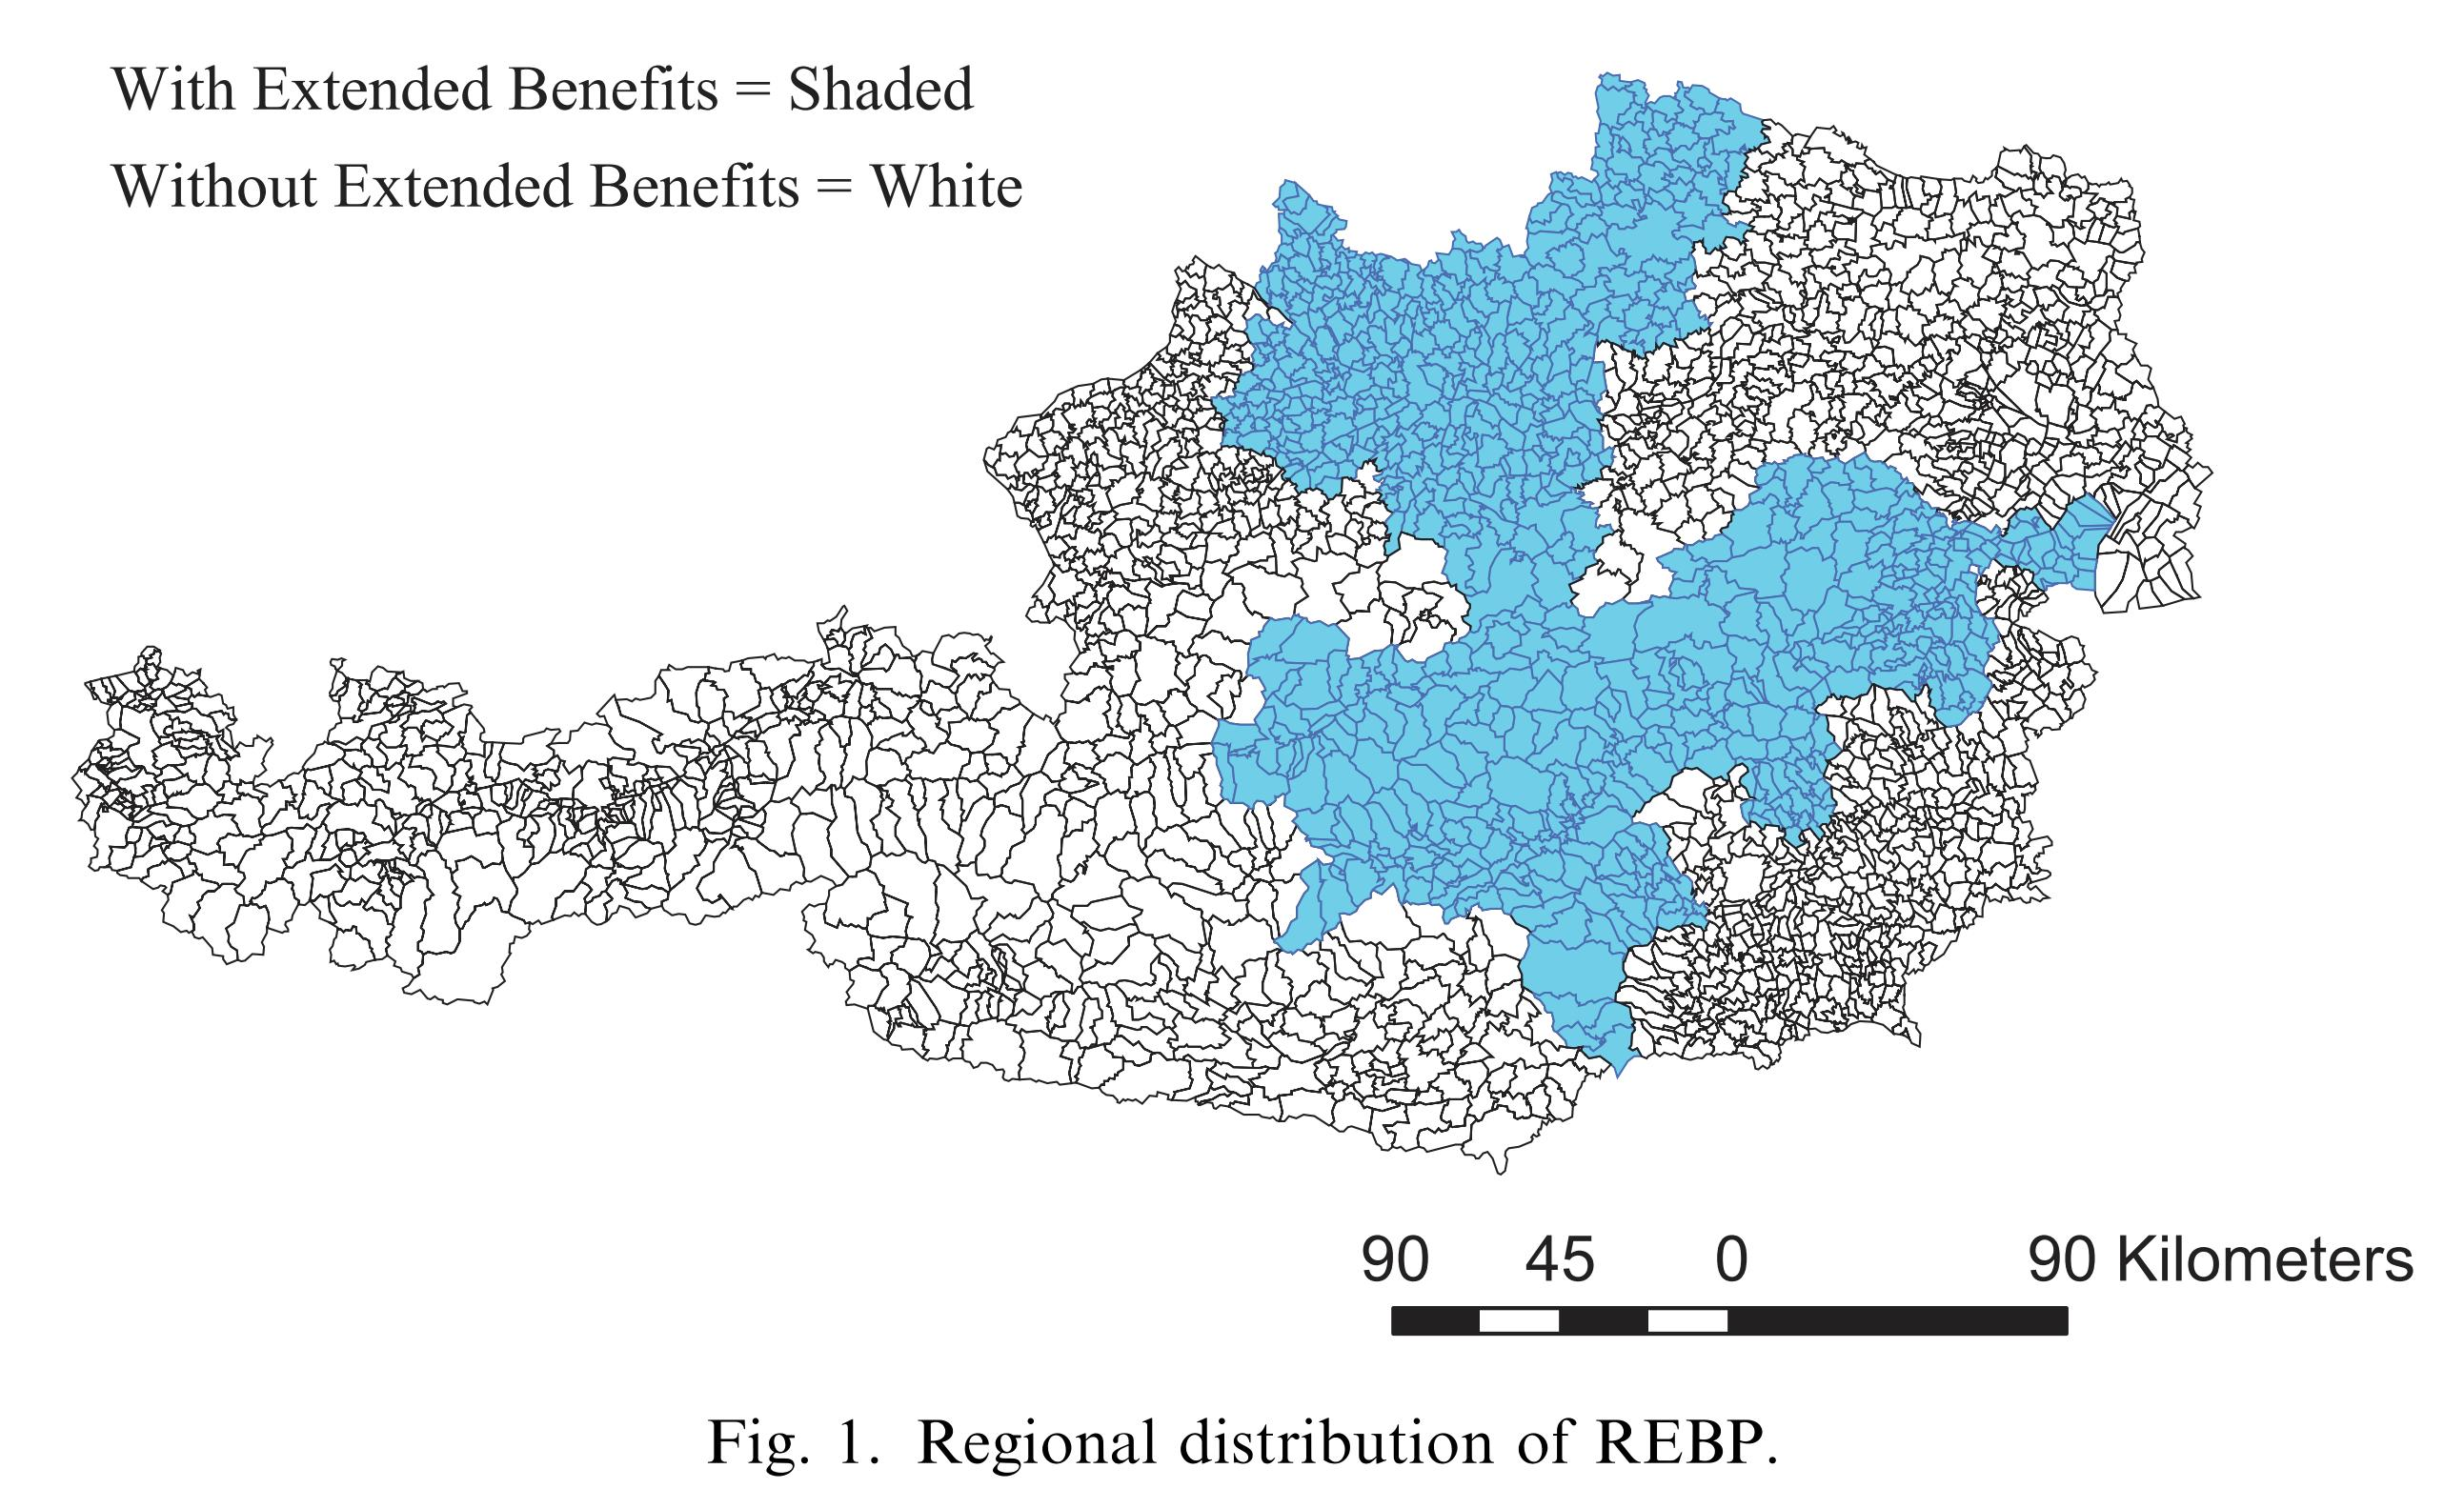
\includegraphics[width=.90\textwidth]{figure/srd_ui_f1.jpg}
	
\end{frame}


\begin{frame}{Spatial Regression Discontinuity Design}{}
	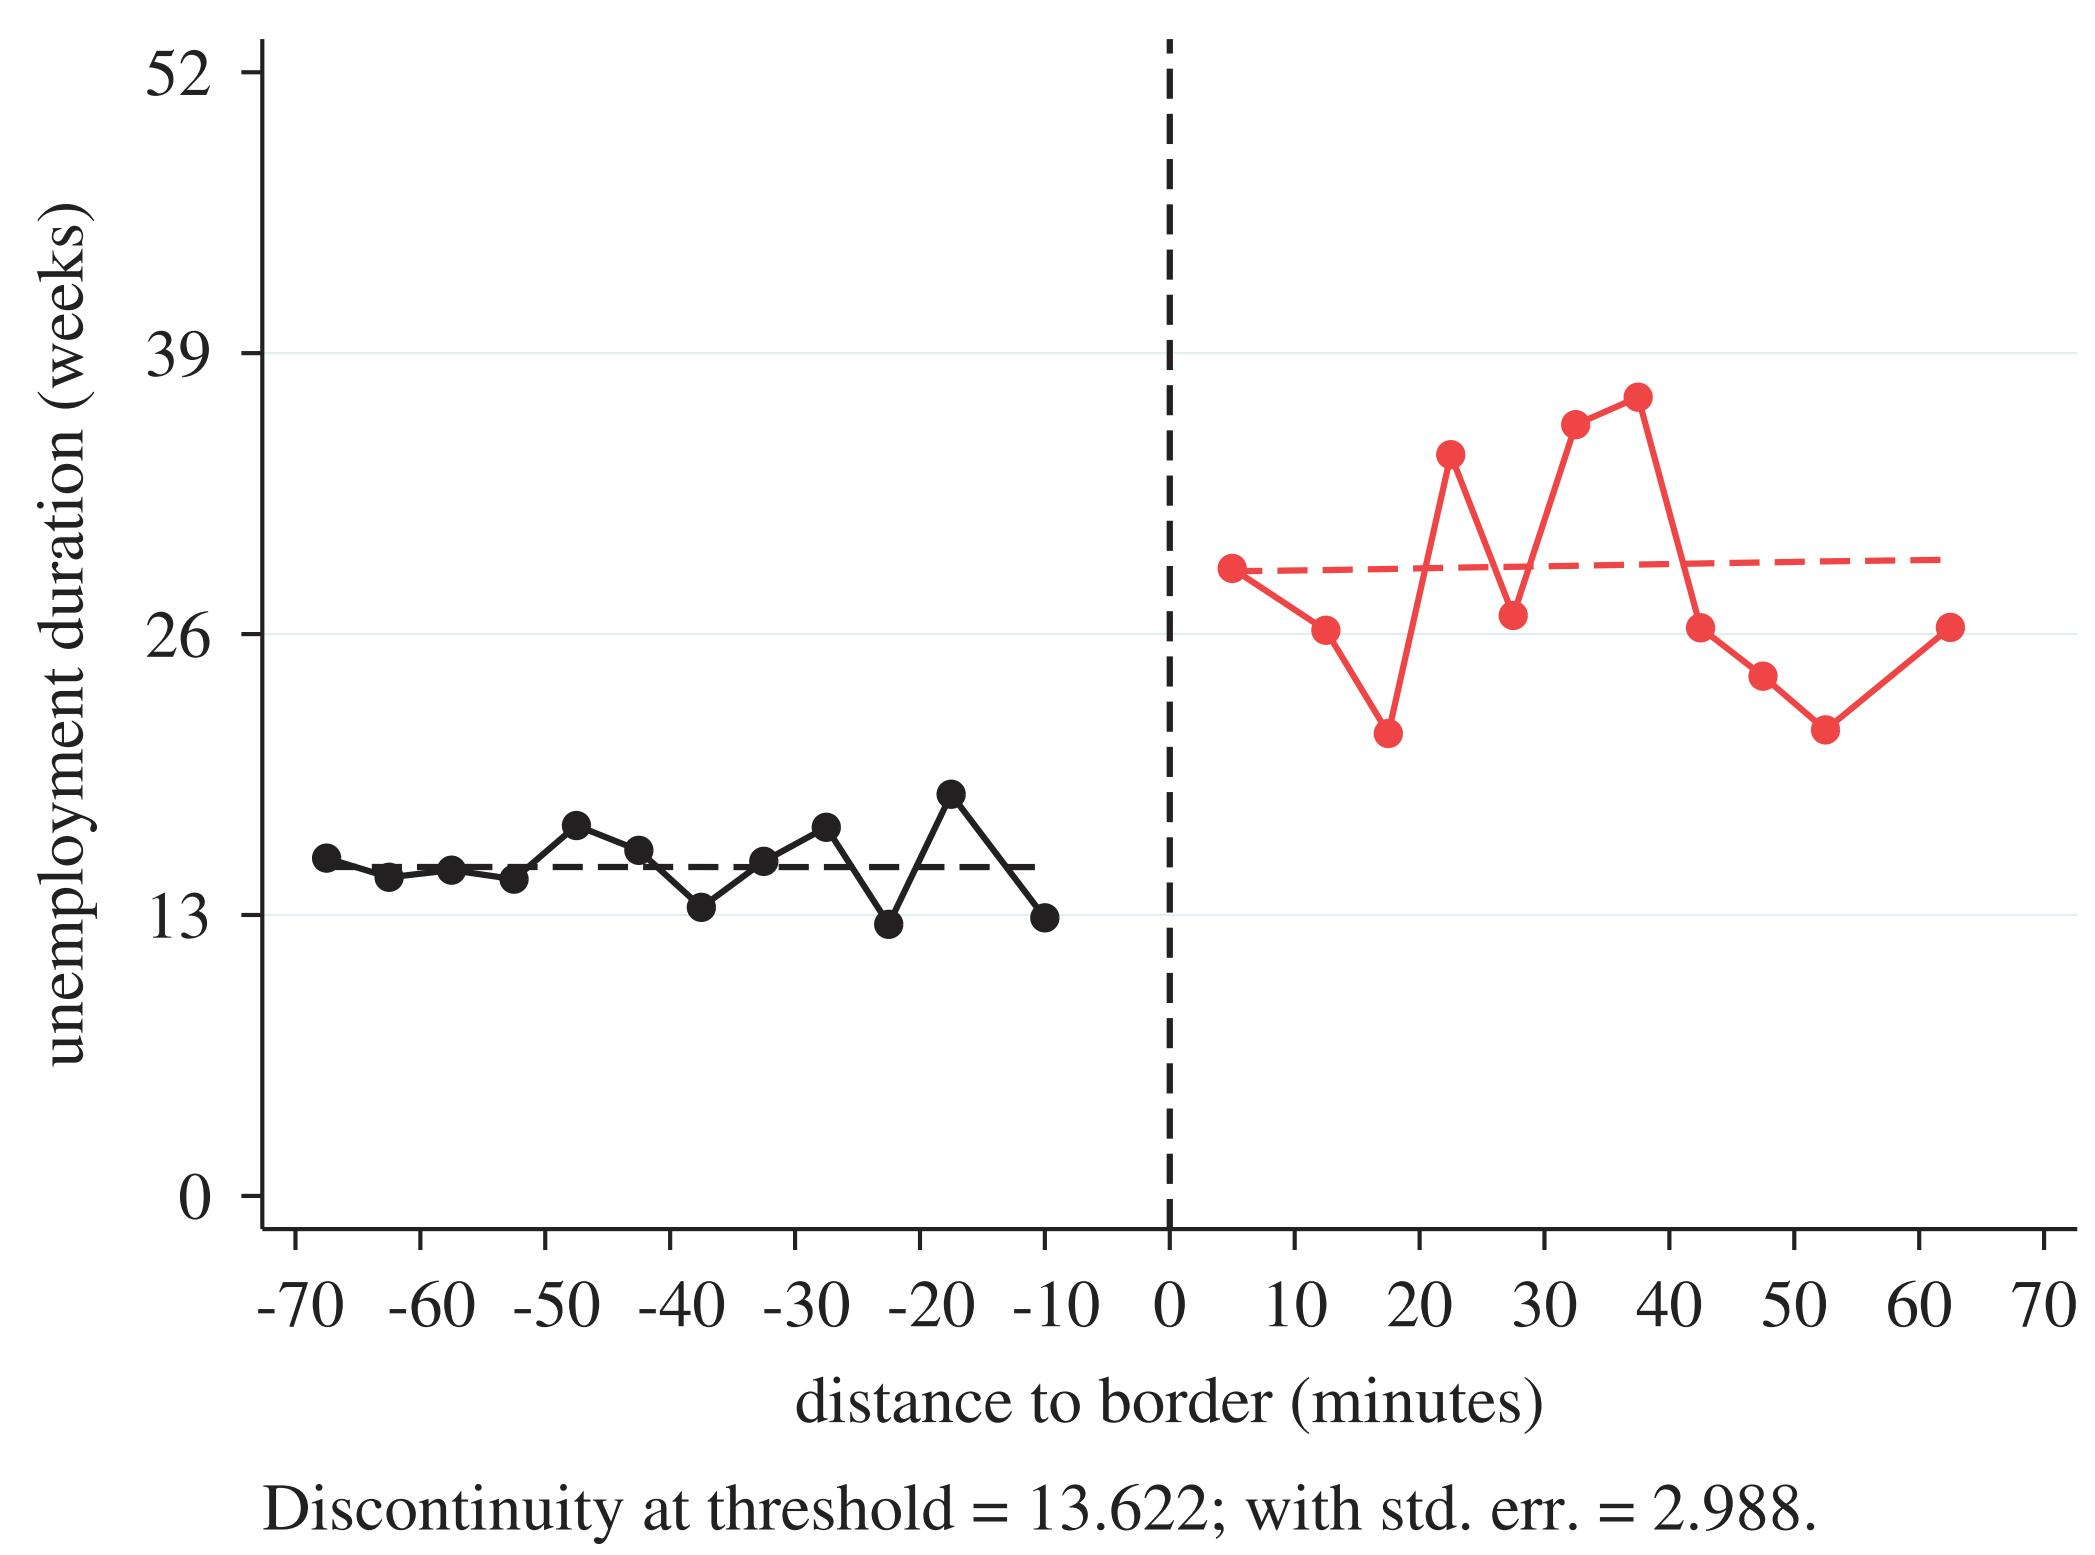
\includegraphics[width=.90\textwidth]{figure/srd_ui_f3.jpg}
	
\end{frame}





 
\title[]  
{Introduction to Spatial Data}
 
 
\author 
{}
 
%\institute{Institute of Economics, Academia Sinica  \\ Econ, NTU}
%\institute{Institute of Economics, Academia Sinica  \\ IMES/IDAS, NCCU}
\institute{}
 
%\author 
%{楊子霆 \\ 中研院經濟所}
 
%\institute 
%{中正大學國際經濟專題研討}
 
 
 
 
\date
{}
 
 
\begin{frame}{}
	\titlepage
\end{frame}
 
 
 
 
 
\begin{frame}{Introduction to Spatial Data}{Overview}
	\begin{itemize}
		\item Spatial data usually focus on \textbf{locations}
		\vspace{0.2cm}
		\item Spatial data (phenomenon) generally have two primary types:
		\vspace{0.2cm}
		\begin{itemize}
			\item[1] Discrete phenomenon
			\vspace{0.2cm}
			\begin{itemize}	
				\item It is also called \textbf{spatial objects}
				\vspace{0.2cm}		
				\item It has boundaries			
				\vspace{0.2cm}
				\item Examples: river, road, country or town
				\vspace{0.2cm}
				\item Usually use \textbf{vector data}			
			\end{itemize}
			\vspace{0.2cm}	
			\item[2]  Continuous phenomenon
			\vspace{0.2cm}	
			\begin{itemize}	
				\item It is also called \textbf{spatial fields}
				\vspace{0.2cm}	
				\item It does not have natural boundaries
				\vspace{0.2cm}
				\item Examples: light intensity at night, elevation, temperature, or air quality (PM 2.5)	
				\vspace{0.2cm}
				\item Usually use \textbf{raster data}	
			\end{itemize}
			
			
			
		\end{itemize}
	\end{itemize}
\end{frame}
 
 
 
 
 
\begin{frame}{Vector Data}{Spatial Objects}
	\begin{itemize}
		\item\textbf{Spatial objects} are usually represented by \textbf{vector data}
		\vspace{0.2cm}
		\item Information about \textbf{spatial objects} can be classified into two categories:
		\begin{itemize}
			\vspace{0.2cm}
			\item Spatial attributes
			\vspace{0.2cm}
			\begin{itemize}
				\item Coordinates that represent its location 
				\vspace{0.2cm}
				\item Coordinates that represent its shape
				\vspace{0.2cm}
			\end{itemize}
			\vspace{0.2cm}
			\item Non-spatial attributes
			\vspace{0.2cm}
			\begin{itemize}
				\item Township name
				\vspace{0.2cm}
				\item Population size  
				\vspace{0.2cm}
				\item GDP per capita 
				\vspace{0.2cm}
			\end{itemize}
			
			
		\end{itemize}
		%\item The \textbf{spatial attributes} of a spatial object consist of one or more pairs of coordinates that represent its shape and/or its location within the study area
		%\vspace{0.2cm}
		%\item The \textbf{non-spatial attributes} of a spatial object consist of its additional features that are relevant to the analysis at hand
		
		
	\end{itemize}
\end{frame}
 
 
 
\begin{frame}{Types of Vector Data}{}
	\begin{itemize}
		\item According to their spatial attributes, \textbf{spatial objects} can be classified into several types
		\vspace{0.2cm}
		\item Here, we focus on two basic types:
		\begin{itemize}
			\vspace{0.2cm}
			\item Points (point data)
			\vspace{0.2cm}
			\item Polygons (area data)
		\end{itemize}
		\vspace{0.2cm}
		\item In all cases, the geometry of these data structures consists
		of sets of \textbf{coordinate pairs (x, y)}
	\end{itemize}
\end{frame}
 
 
 
\begin{frame}{Vector Data}{Points}
	\begin{minipage}{0.6\linewidth}
		\begin{itemize}
			\item A point $s_i$ is a spatial object located within study area $\mathcal{A}$ at coordinates ($s_{i1}, s_{i2}$)
			\vspace{0.2cm}
			\item Points can represent the following real entities:
			\vspace{0.2cm}
			\begin{itemize}
				\item Buildings
				\vspace{0.2cm}
				\item Places where specific events took place
				\vspace{0.2cm}
				\item Pollution sources
			\end{itemize}
			\vspace{0.2cm}
			\item Each point might also have \textbf{non-spatial attributes}, such as household size or number of people.
		\end{itemize}
	\end{minipage}
	\hspace{0.02\linewidth}
	\begin{minipage}{0.3\linewidth}
		\begin{figure}[H]
			\scalebox{1}{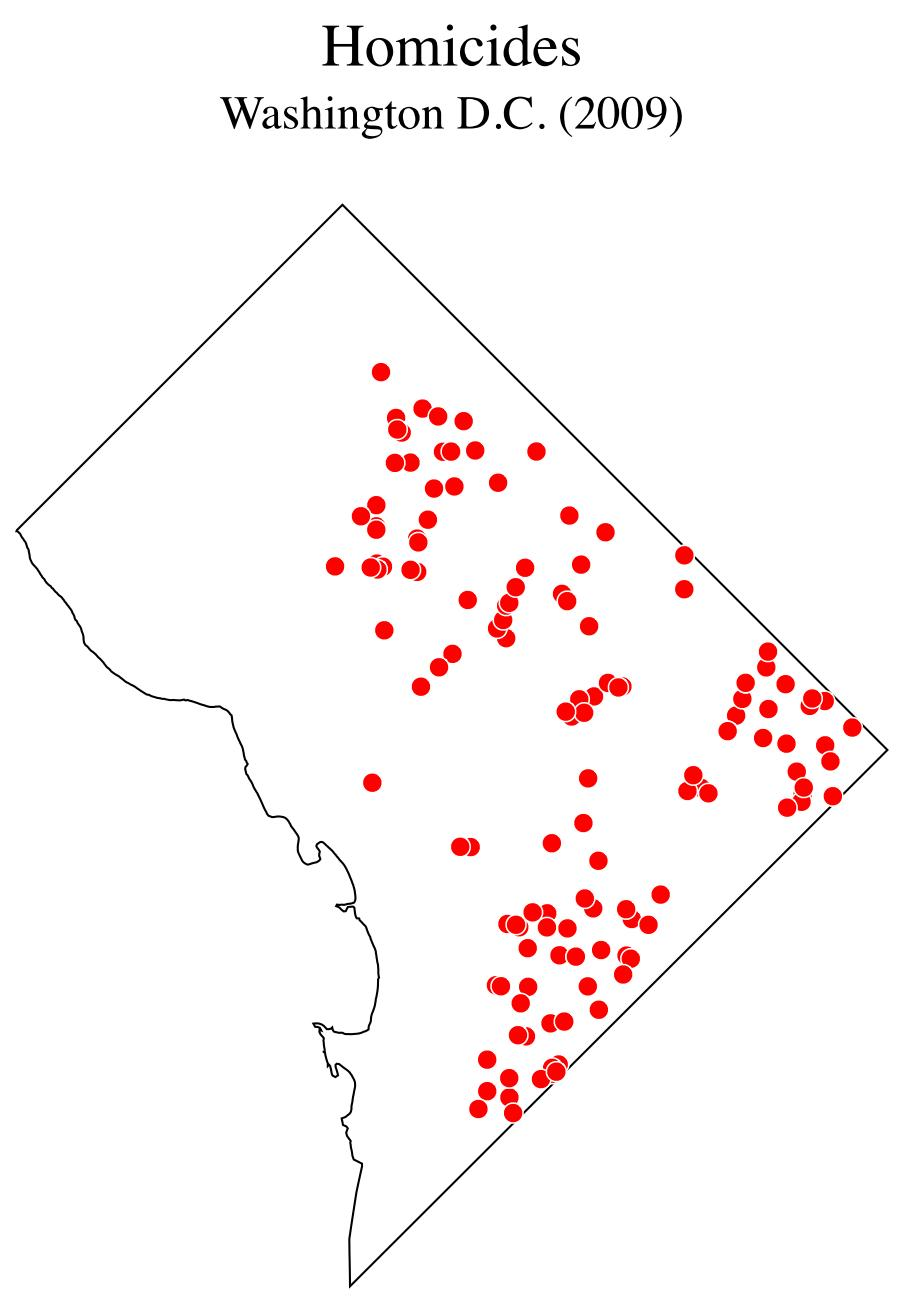
\includegraphics{figure/stata_spatial-1.jpg}}
		\end{figure}
	\end{minipage}
\end{frame}
 
 
 
\begin{frame}{Vector Data}{Polygons}
	\begin{minipage}{0.6\linewidth}
		\begin{itemize}
			\item A polygon $r_i$ is a \textit{region} of study area $\mathcal{A}$ bounded by a closed polygonal chain 
			\vspace{0.2cm}
			\item It can be defined by the coordinate set $\{(r_{i1(1)},r_{i2(1)}),(r_{i1(2)},r_{i2(2)}),...$, $(r_{i1(m)},r_{i2(m)}),...,(r_{i1(M)},r_{i2(M)})\}$, where $r_{i1(1)}=r_{i1(M)}$ and $r_{i2(1)}=r_{i2(M)}$
			\vspace{0.2cm}
			\item Polygons can represent several kinds of real entities:
			\vspace{0.2cm}
			\begin{itemize}
				\item States, counties, electoral districts
				\vspace{0.2cm}
				%\item Provinces
				\item Parks, lakes
				%\item Census tracts
				%\item Electoral districts
			\end{itemize}
			
		\end{itemize}
	\end{minipage}
	\hspace{0.02\linewidth}
	\begin{minipage}{0.3\linewidth}
		\begin{figure}[H]
			\scalebox{1}{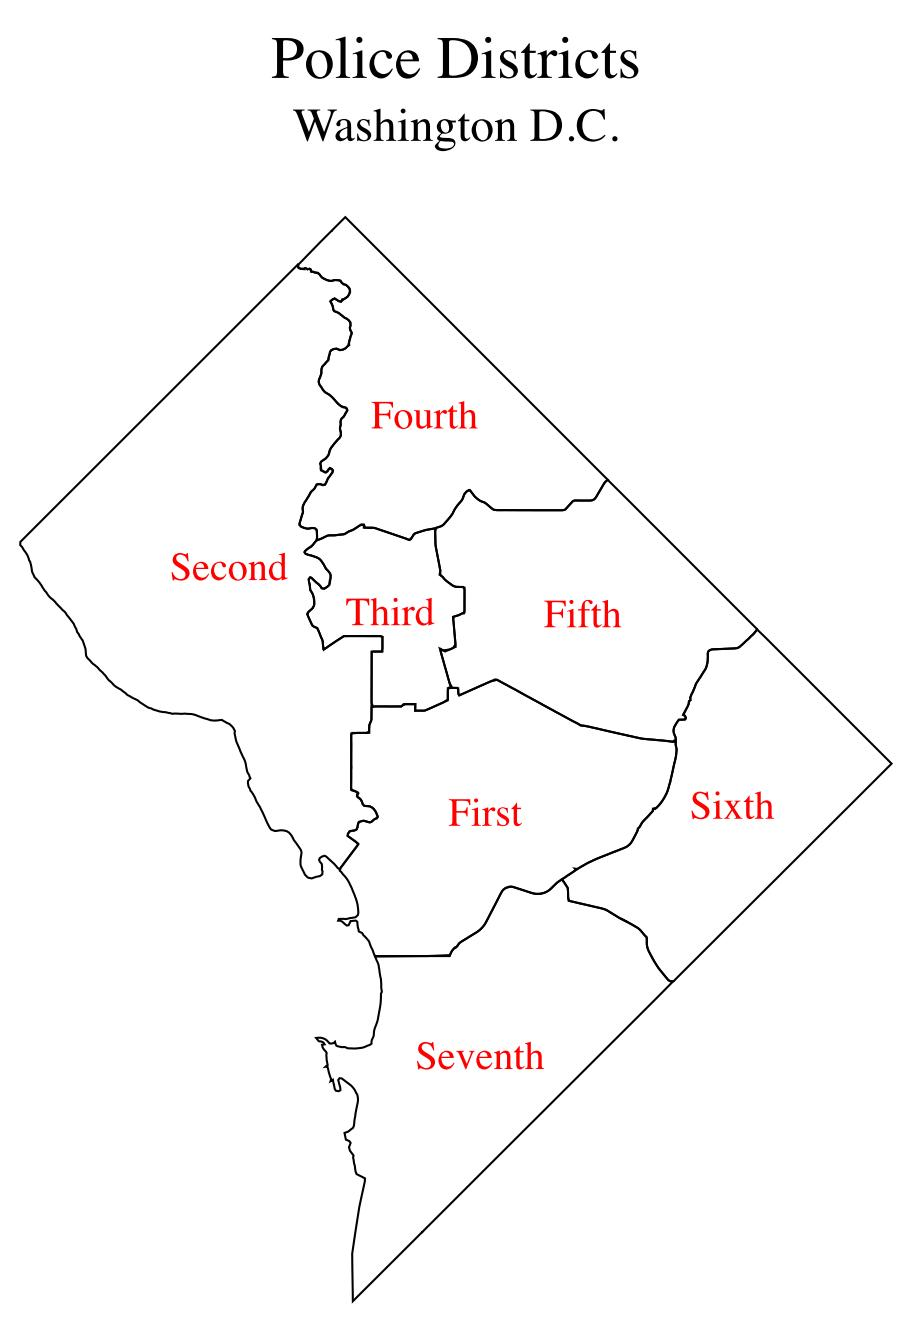
\includegraphics{figure/stata_spatial-2.jpg}}
			%\scalebox{1}{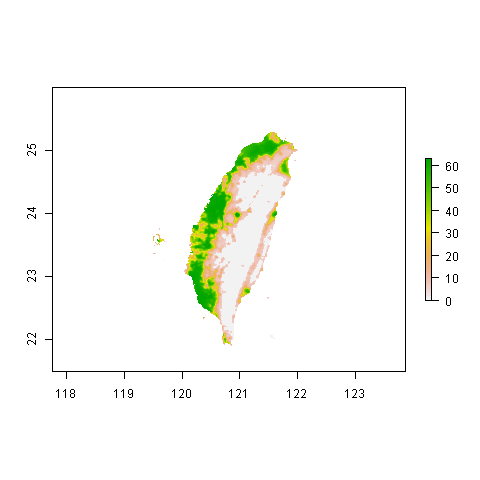
\includegraphics[width=.8\textwidth]{figure/TWN_2013.png}}
		\end{figure}
	\end{minipage}
\end{frame}
 
 
 
 
 
\begin{frame}{Raster Data}{Spatial Fields}
	\begin{itemize}
		\item\textbf{Spatial fields} are usually represented by \textbf{raster data}
		\vspace{0.2cm}
		\item Raster data is commonly used to represent continuous variables
		\begin{itemize}
			\vspace{0.2cm}
			\item A raster divides the world into a grid of equally sized
			rectangles (i.e. grid cells or pixels)
			\vspace{0.2cm}
			\item These rectangles all have a values (or a missing value) for the variables of interest
			\vspace{0.2cm}
			\item A raster cell/pixel value should normally represent the value for the area it covers
				\begin{itemize}
					\item \textbf{Average}: for continuous variables (e.g., temperature, elevation)
					\item \textbf{Majority}: for categorical variables (e.g., land use type)
				\end{itemize}
		\end{itemize}
		
		
	\end{itemize}
\end{frame}
 
 
 
 
 
\begin{frame}{Raster Data}{Night Light from Satellite Images}
	\begin{minipage}{0.6\linewidth}
		\begin{itemize}
			\item Each raster pixel value in a \textbf{DMSP/OLS} satellite image ranges from 0 to 63 (Digital Number)
				\vspace{0.2cm}
				\item It represents the light intensity at night in Taiwan
			
		\end{itemize}
	\end{minipage}
	\hspace{0.02\linewidth}
	\begin{minipage}{0.3\linewidth}
		\begin{figure}[H]
			%\scalebox{1}{
\includegraphics{stata_spatial-2.jpg}}
			\scalebox{1.5}{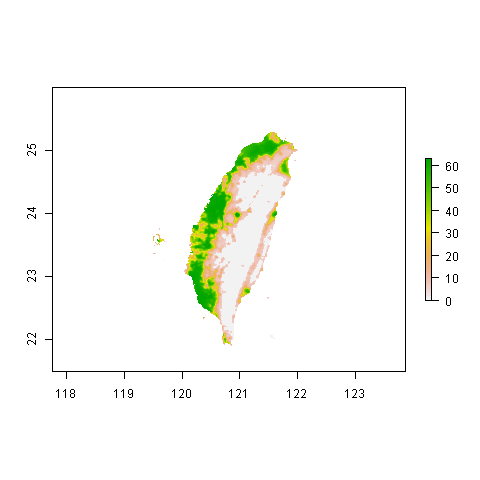
\includegraphics[width=1.0\textwidth]{figure/TWN_2013.png}}
		\end{figure}
	\end{minipage}
\end{frame}
 
 
 
\begin{frame}{Night Light from Satellite Images}{Taiwan in 1992}
	\begin{center}
		\begin{figure}[p]
			\centering
			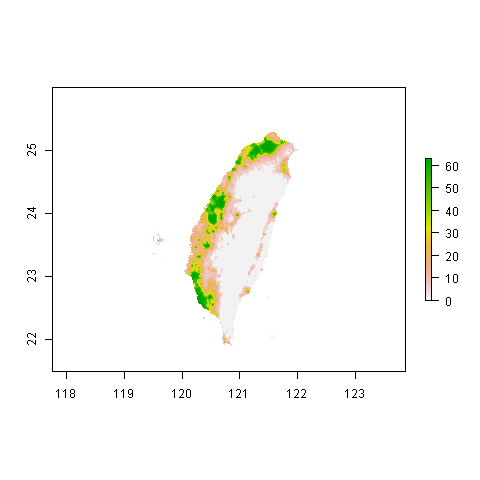
\includegraphics[width=.8\textwidth]{figure/TWN_1992.png}
		\end{figure}
	\end{center}
\end{frame}
 
\begin{frame}{Night Light from Satellite Images}{Taiwan in 2013}
	\begin{center}
		\begin{figure}[p]
			\centering
			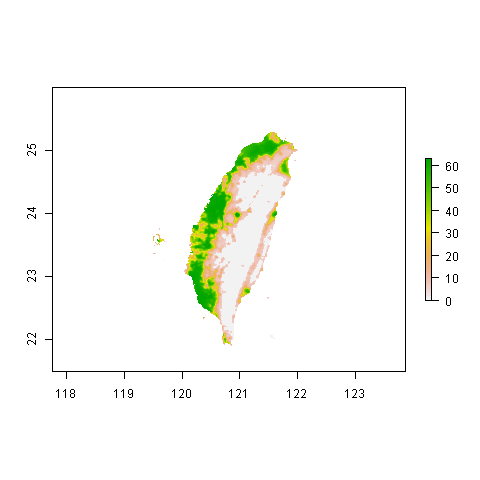
\includegraphics[width=.8\textwidth]{figure/TWN_2013.png}
		\end{figure}
	\end{center}
\end{frame}
 
 
 
 
\begin{frame}{Night Light from Satellite Images}{Kinmen in 1992}
	\begin{center}
		\begin{figure}[p]
			\centering
			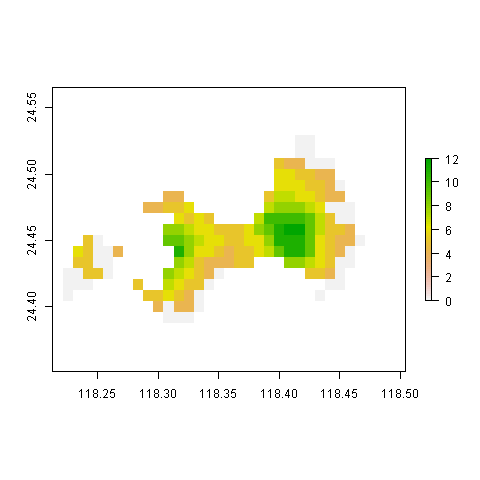
\includegraphics[width=.8\textwidth]{figure/KMM_1992.png}
		\end{figure}
	\end{center}
\end{frame}
 
\begin{frame}{Night Light from Satellite Images}{Kinmen in 2013}
	\begin{center}
		\begin{figure}[p]
			\centering
			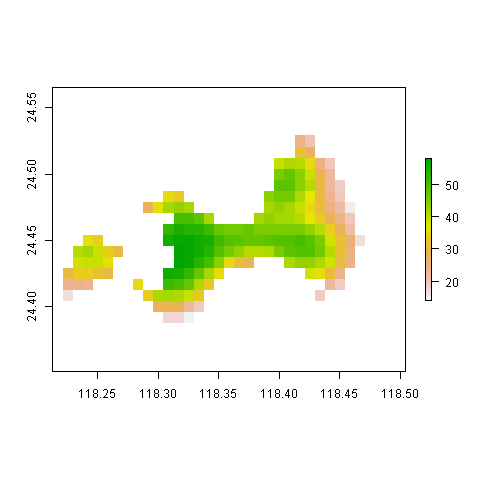
\includegraphics[width=.8\textwidth]{figure/KMM_2013.png}
		\end{figure}
	\end{center}
\end{frame}
 


\title[]  
{Spatial Data and Coordinate Systems}
 
 
\author 
{}
 
%\institute{Institute of Economics, Academia Sinica  \\ Econ, NTU}
%\institute{Institute of Economics, Academia Sinica  \\ IMES/IDAS, NCCU}
\institute{}
 
%\author 
%{楊子霆 \\ 中研院經濟所}
 
%\institute 
%{中正大學國際經濟專題研討}
 
 
 
 
\date
{}
 
 
\begin{frame}{}
	\titlepage
\end{frame}
 
 
 
 
\begin{frame}{Coordinate Systems}
	\begin{itemize}
		%\item Before discussing how to create maps using STATA, it is critical to acquire a basic understanding of projections
		%	\vspace{0.2cm}
		\item The distinguishing feature of spatial data is that each data point has a \textbf{geographic identifier} attached to it
		\vspace{0.2cm}
		\item To view and manipulate your data, these identifiers will need to be referenced to a \textbf{coordinate system}
		\vspace{0.2cm}
		\item Using the wrong coordinate system is a critical mistake that can
		result in your calculations being complete garbage
	\end{itemize}
\end{frame}
 
 
 
 
 
\begin{frame}{Coordinate Systems}
	\begin{itemize}
		\item Two types of coordinate systems:
		\vspace{0.2cm}
		\begin{itemize}
			\item[1] Geographic coordinate systems
			\vspace{0.2cm}	
			\begin{itemize}
				\item Three dimensional angular system
			\end{itemize}
			\vspace{0.2cm}	
			\item[2] Projected coordinate systems
			\vspace{0.2cm}	
			\begin{itemize}
				\item Two dimensional planar system
			\end{itemize}
			
		\end{itemize}
		
	\end{itemize}
\end{frame}
 
 
 
 
 
 
\begin{frame}{Geographic Coordinate Systems}
	\begin{itemize}
		\item In geographic coordinate systems (GCS), each location is coded by \textbf{angle} from \textbf{earth center}
		\vspace{0.2cm}
		\item The unit of measure in geographic coordinate systems is \textbf{decimal degrees}	
		\begin{itemize}
			\vspace{0.2cm}
			\item Taipei: $24.5723^{o}$ N (latitude) and $121.3213^{o}$ E (longitude)
			\vspace{0.2cm}
			\item Stockholm: $59.3293^{o}$ N and $18.0686^{o}$ E 
		\end{itemize}
		\vspace{0.2cm}
		\item As with latitude and longitude, the values are bounded by $-90^{o}$ to $90^{o}$ and $-180^{o}$ to $180^{o}$ respectively.
		\vspace{0.2cm}
		\item Latitude and longitude are usually expressed in that sequence, latitude before longitude
		
	\end{itemize}
\end{frame}
 
 
 
\begin{frame}{Geographic Coordinate Systems}{}
	
	\begin{center}
		\begin{figure}[p]
			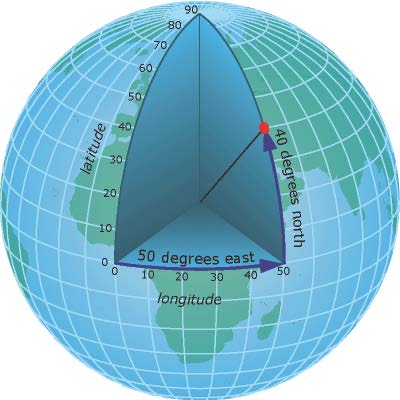
\includegraphics[width=.65\textwidth]{figure/GCS_pic_arc_gis.jpg}
		\end{figure}
		\begin{minipage}{0.9\linewidth}
			\fontsize{8}{8pt}\selectfont
			\emph{Source:} ArcGIS for Desktop
		\end{minipage}	
	\end{center}
\end{frame}
 
 
 
 
 
\begin{frame}{Geographic Coordinate Systems}
	\begin{itemize}
		
		\item Latitudes:
		\vspace{0.2cm}
		\begin{itemize}
			\item North of the equator: Positive
			\vspace{0.2cm}
			\item South of the equator: Negative
		\end{itemize}
		\vspace{0.2cm}
		\item Longitudes:
		\vspace{0.2cm}
		\begin{itemize}
			\item East of Prime Meridian: Positive
			\vspace{0.2cm}
			\item West of Prime Meridian: Negative
		\end{itemize}
		
	\end{itemize}
\end{frame}
 
 
 
 
\begin{frame}{Geographic Coordinate Systems}
	\begin{itemize}
		
		\item Most popular GCS: 
		\begin{itemize}
			\vspace{0.2cm}
			\item World Geodetic System (\textbf{WGS 1984})
			\vspace{0.2cm}
			\item WGS 1984 is a coordinate system designed by the U.S. military
		\end{itemize}
		\vspace{0.2cm}
		\item GCS used in Taiwan:
		\vspace{0.2cm}
		\begin{itemize}
			\item \textbf{TWD97}: current standard adopted in 1997; closely aligned with WGS 1984 --- use this for new projects
			\vspace{0.2cm}
			\item \textbf{TWD67}: older standard; coordinates can differ from TWD97 by \textasciitilde{}200--800 meters --- mixing the two causes errors
		\end{itemize}
		
	\end{itemize}
\end{frame}
 
 
 
%As with latitude and longitude, the values are bounded by $\pm$90$^\circ$ and $\pm$180$^\circ$ respectively.
 
%Positive latitudes are north of the equator, negative latitudes are south of the equator. Positive longitudes are east of Prime Meridian, negative longitudes are west of the Prime Meridian. Latitude and longitude are usually expressed in that sequence, latitude before longitude.
 
 
 
 
\begin{frame}{Geographic Coordinate Systems}
	\begin{itemize}
		
		\item Although longitude and latitude can locate exact positions on the surface of the globe, they are NOT uniform units of measure
		\vspace{0.2cm}
		\begin{itemize}
			\item The circumference of the Earth at the equator is 40,075,161.2 meters
			\vspace{0.2cm}
			\item The equator is divided into 360 degrees of longitude
			\vspace{0.2cm}
			\item So each degree at the equator represents 111,319.9 meters or approximately 111.32 km
			\vspace{0.2cm}
			\item One degree of \textbf{latitude} is also $\approx$ 111 km everywhere --- it is nearly constant
			\vspace{0.2cm}
			\item One degree of \textbf{longitude} varies: $\approx$ 111 km at the equator, but \textbf{shrinks toward zero} at the poles
		\end{itemize}
		
	\end{itemize}
\end{frame}
 
 
 
\begin{frame}{Geographic Coordinate Systems}
	\begin{itemize}
		\item Only along the equator does the distance represented by \textbf{one degree of longitude} approximate the distance represented by \textbf{one degree of latitude}
		\vspace{0.2cm}
		\item As the meridians converge toward the poles, the distance represented by \textbf{one degree of longitude decreases to zero}
		\vspace{0.2cm}	
		\item A major question in spatial analysis is how to transform this \textbf{three dimensional angular system} to a \textbf{two dimensional planar system}
		
		%\item We need to use some math models to calculate distance based on a \textbf{geographic coordinate system}
		%\item You should NOT do distance or area calculations on data that is in a \textbf{geographic coordinate system}
	\end{itemize}
\end{frame}
 
 
 
%\begin{frame}{Geographic Coordinate Systems}{}
%	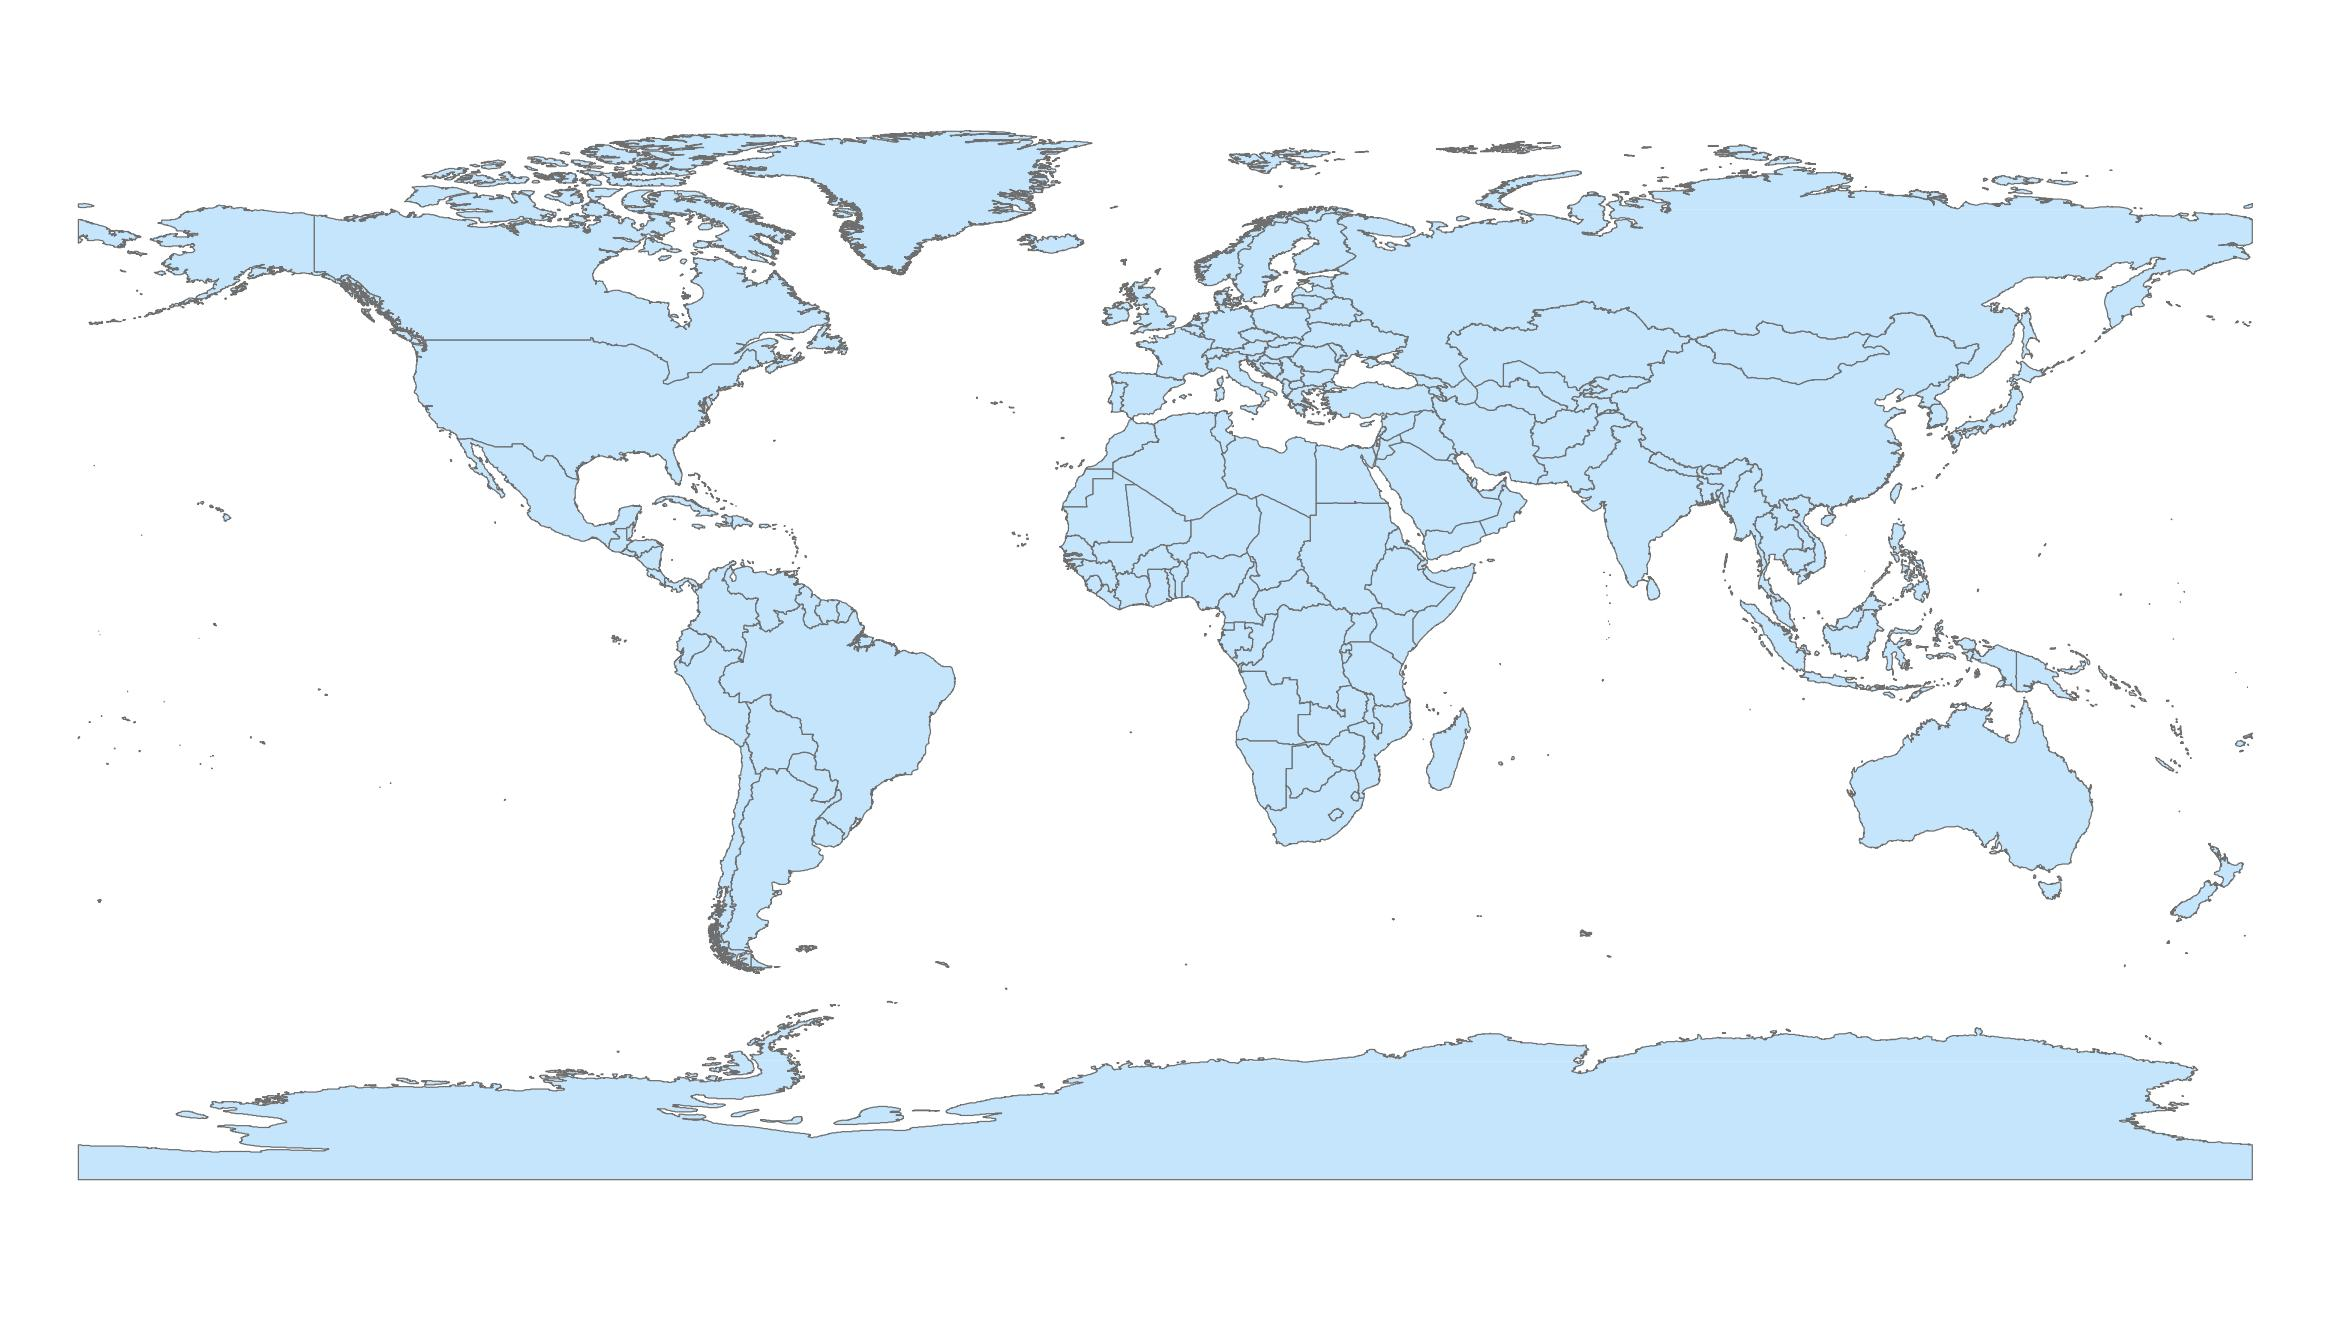
\includegraphics[width=.90\textwidth]{figure/geo_c_s.jpg}
 
%\end{frame}
 
 
 
 
\begin{frame}{Projected Coordinate Systems}
	\begin{itemize}
		\item \textbf{Projected coordinate systems} project the \textbf{round surface} of the earth (in degrees) onto a \textbf{flat surface} (two-dimensional)
		\vspace{0.2cm}
		\item A \textbf{projected coordinate system} is always based on a \textbf{geographic coordinate system}
		\vspace{0.2cm}
		\item Unlike a geographic coordinate system, a projected coordinate system has constant lengths, angles, and areas across the two dimensions
		\vspace{0.2cm}
		\item The unit of measure in a projected coordinate system is the \textbf{meter}
		
		%\begin{itemize}
		%	\item UTM projections
		%		\vspace{0.2cm}
		%	\item Goodes projection
		%	    	\vspace{0.2cm}
		%	\item Equidistant cylindrical projection
		%		\vspace{0.2cm}
		%	\item Cylindrical Equal Area
		%		\end{itemize}
\end{itemize}
\end{frame}
 
 
\begin{frame}{Projected Coordinate Systems}
\begin{itemize}
	
	%\item Locations are identified by x,y coordinates on a grid, with the origin at the center of the grid 
	%\vspace{0.2cm}
	\item Each position has two values (x,y coordinates) that reference it to that central location
	\vspace{0.2cm}
	\begin{itemize}
		\item x specifies its horizontal position and y specifies its vertical position
		\vspace{0.2cm}
		\item The two values are called the x-coordinate and y-coordinate. 
		\vspace{0.2cm}
		\item The coordinates at the origin are x = 0 and y = 0
	\end{itemize}
	\vspace{0.2cm}
	\item All projections introduce some distortions --- think of peeling an orange and trying to lay the skin flat
	\vspace{0.2cm}
	\item Different projections preserve different properties:
	\vspace{0.2cm}
	\begin{itemize}
		\item \textbf{Shape} (conformal): angles are correct, e.g., Google Maps
		\vspace{0.1cm}
		\item \textbf{Area} (equal-area): useful for comparing region sizes
		\vspace{0.1cm}
		\item \textbf{Distance} (equidistant): distances from a reference point are correct
		\vspace{0.1cm}
		\item \textbf{Direction} (azimuthal): bearings from center are correct
	\end{itemize}
	
\end{itemize}
\vspace{0.2cm}
\begin{alertblock}{Key point}
	No single projection can preserve all properties simultaneously --- choose based on your research purpose
\end{alertblock}
\end{frame}
 
 
 
 
\begin{frame}{Projected Coordinate Systems}{Common Examples}
\begin{itemize}
	\item \textbf{UTM (Universal Transverse Mercator)}
	\vspace{0.1cm}
	\begin{itemize}
		\item Divides the world into 60 zones; each zone uses meters as the unit
		\vspace{0.1cm}
		\item Taiwan is in \textbf{Zone 51N}
		\vspace{0.1cm}
		\item Widely used in global research; minimizes distortion within each zone
	\end{itemize}
	\vspace{0.3cm}
	\item \textbf{TWD97 / TM2} (Taiwan-specific)
	\vspace{0.1cm}
	\begin{itemize}
		\item Official projected coordinate system for Taiwan
		\vspace{0.1cm}
		\item Based on Transverse Mercator projection; unit is \textbf{meters}
		\vspace{0.1cm}
		\item Used in government maps, land administration, and most Taiwan GIS data
		\vspace{0.1cm}
		\item \textbf{Practical tip}: when working with Taiwan data, always check whether the file uses TWD97 (degrees) or TWD97/TM2 (meters)
	\end{itemize}
 
\end{itemize}
\end{frame}
 
 
 



\title[]  
{Spatial Data Analysis and R}


\author 
{}

%\institute{Institute of Economics, Academia Sinica  \\ Econ, NTU}
%\institute{Institute of Economics, Academia Sinica  \\ IMES/IDAS, NCCU}
\institute{}

%\author 
%{楊子霆 \\ 中研院經濟所}

%\institute 
%{中正大學國際經濟專題研討}




\date
{}


\begin{frame}{}
\titlepage
\end{frame}





\begin{frame}{Why R for Spatial Analysis?}


\begin{itemize}
	\item R is a powerful tool for spatial analysis
				\vspace{0.2cm}
	\item \textbf{Open Source:} R is freely available and has a large user community.
				\vspace{0.2cm}
	\item \textbf{Comprehensive Packages:} R has numerous packages for spatial analysis (e.g., \texttt{sf}, \texttt{spatial}, \texttt{raster}).
				\vspace{0.2cm}
	\item \textbf{Data Visualization:} R offers excellent data visualization capabilities for spatial data.
	
	
\end{itemize}


\end{frame}



\begin{frame}{Why R for Spatial Analysis?}


\begin{itemize}
\item \textbf{Integration:} R seamlessly integrates with other data analysis and statistical tools.
				\vspace{0.2cm}
\item \textbf{Reproducibility:} R allows for reproducible research through scripts (programming)
				\vspace{0.2cm}
\begin{itemize}
\item Clicking the ArcGIS (or QGIS) user interface is a waste of time from the perspective of academic productivity
				\vspace{0.2cm}
			\end{itemize}
\item \textbf{Community Support:} Active R user community provides help and resources.
	\vspace{0.2cm}
\begin{itemize}
	\item Chatgpt can help, too
	\vspace{0.2cm}
\end{itemize}


	
\end{itemize}


\end{frame}



\begin{frame}[fragile]{sf Package}{Load required packages}

\begin{lstlisting}
install.packages("pacman")
library(pacman)
p_load(
dplyr, tidyverse, sf, rdrobust, readxl, fastDummies, writexl, readr
)
\end{lstlisting}
\begin{itemize}
	\item In R, we use \textbf{sf} package to handle and operate on spatial datasets
	\vspace{0.2cm}
	\item The \textbf{sf} package uses the class of simple feature (sf) for spatial objects in R
	
\end{itemize}

\end{frame}


\begin{frame}[fragile]{Path}

\begin{lstlisting}
path <- "C:\\nest\\Dropbox\\Courses\\Causal_Inference_Big_Data\\Slides\\L10_spatial_data_analysis\\data\\"
path_mrt_line <- str_c(path, "MRT_1120412.csv")
path_house    <- str_c(path, "taipei_housing.csv")
\end{lstlisting}

\end{frame}


\title[]  
{Spatial Data Structure}


\author 
{}

%\institute{Institute of Economics, Academia Sinica  \\ Econ, NTU}
%\institute{Institute of Economics, Academia Sinica  \\ IMES/IDAS, NCCU}
\institute{}

%\author 
%{楊子霆 \\ 中研院經濟所}

%\institute 
%{中正大學國際經濟專題研討}




\date
{}


\begin{frame}{}
	\titlepage
\end{frame}




\begin{frame}[fragile]{Spatial Data}{Points}
\begin{lstlisting}
one_p   <- st_point(c(0, 0))
multi_p <- st_multipoint(rbind(c(1, 1), c(0, 1)))
\end{lstlisting}
\begin{itemize}
	\item \textbf{st\_point} creates a single spatial point with coordinates (0, 0) and assigns it to the variable `one\_p`.
				\vspace{0.2cm}
	\item \textbf{st\_multipoint} creates a multipoint geometry with two points: (1, 1) and (0, 1) 
				\vspace{0.2cm}
				\begin{itemize}
	\item It uses `\textbf{rbind}` to combine the coordinates into a matrix and assigns the result to the variable `multi\_p`.
\end{itemize}
\end{itemize}
\end{frame}



\begin{frame}[fragile]{Spatial Data}{Points}
\begin{center}
	\begin{figure}[p]
		\centering
		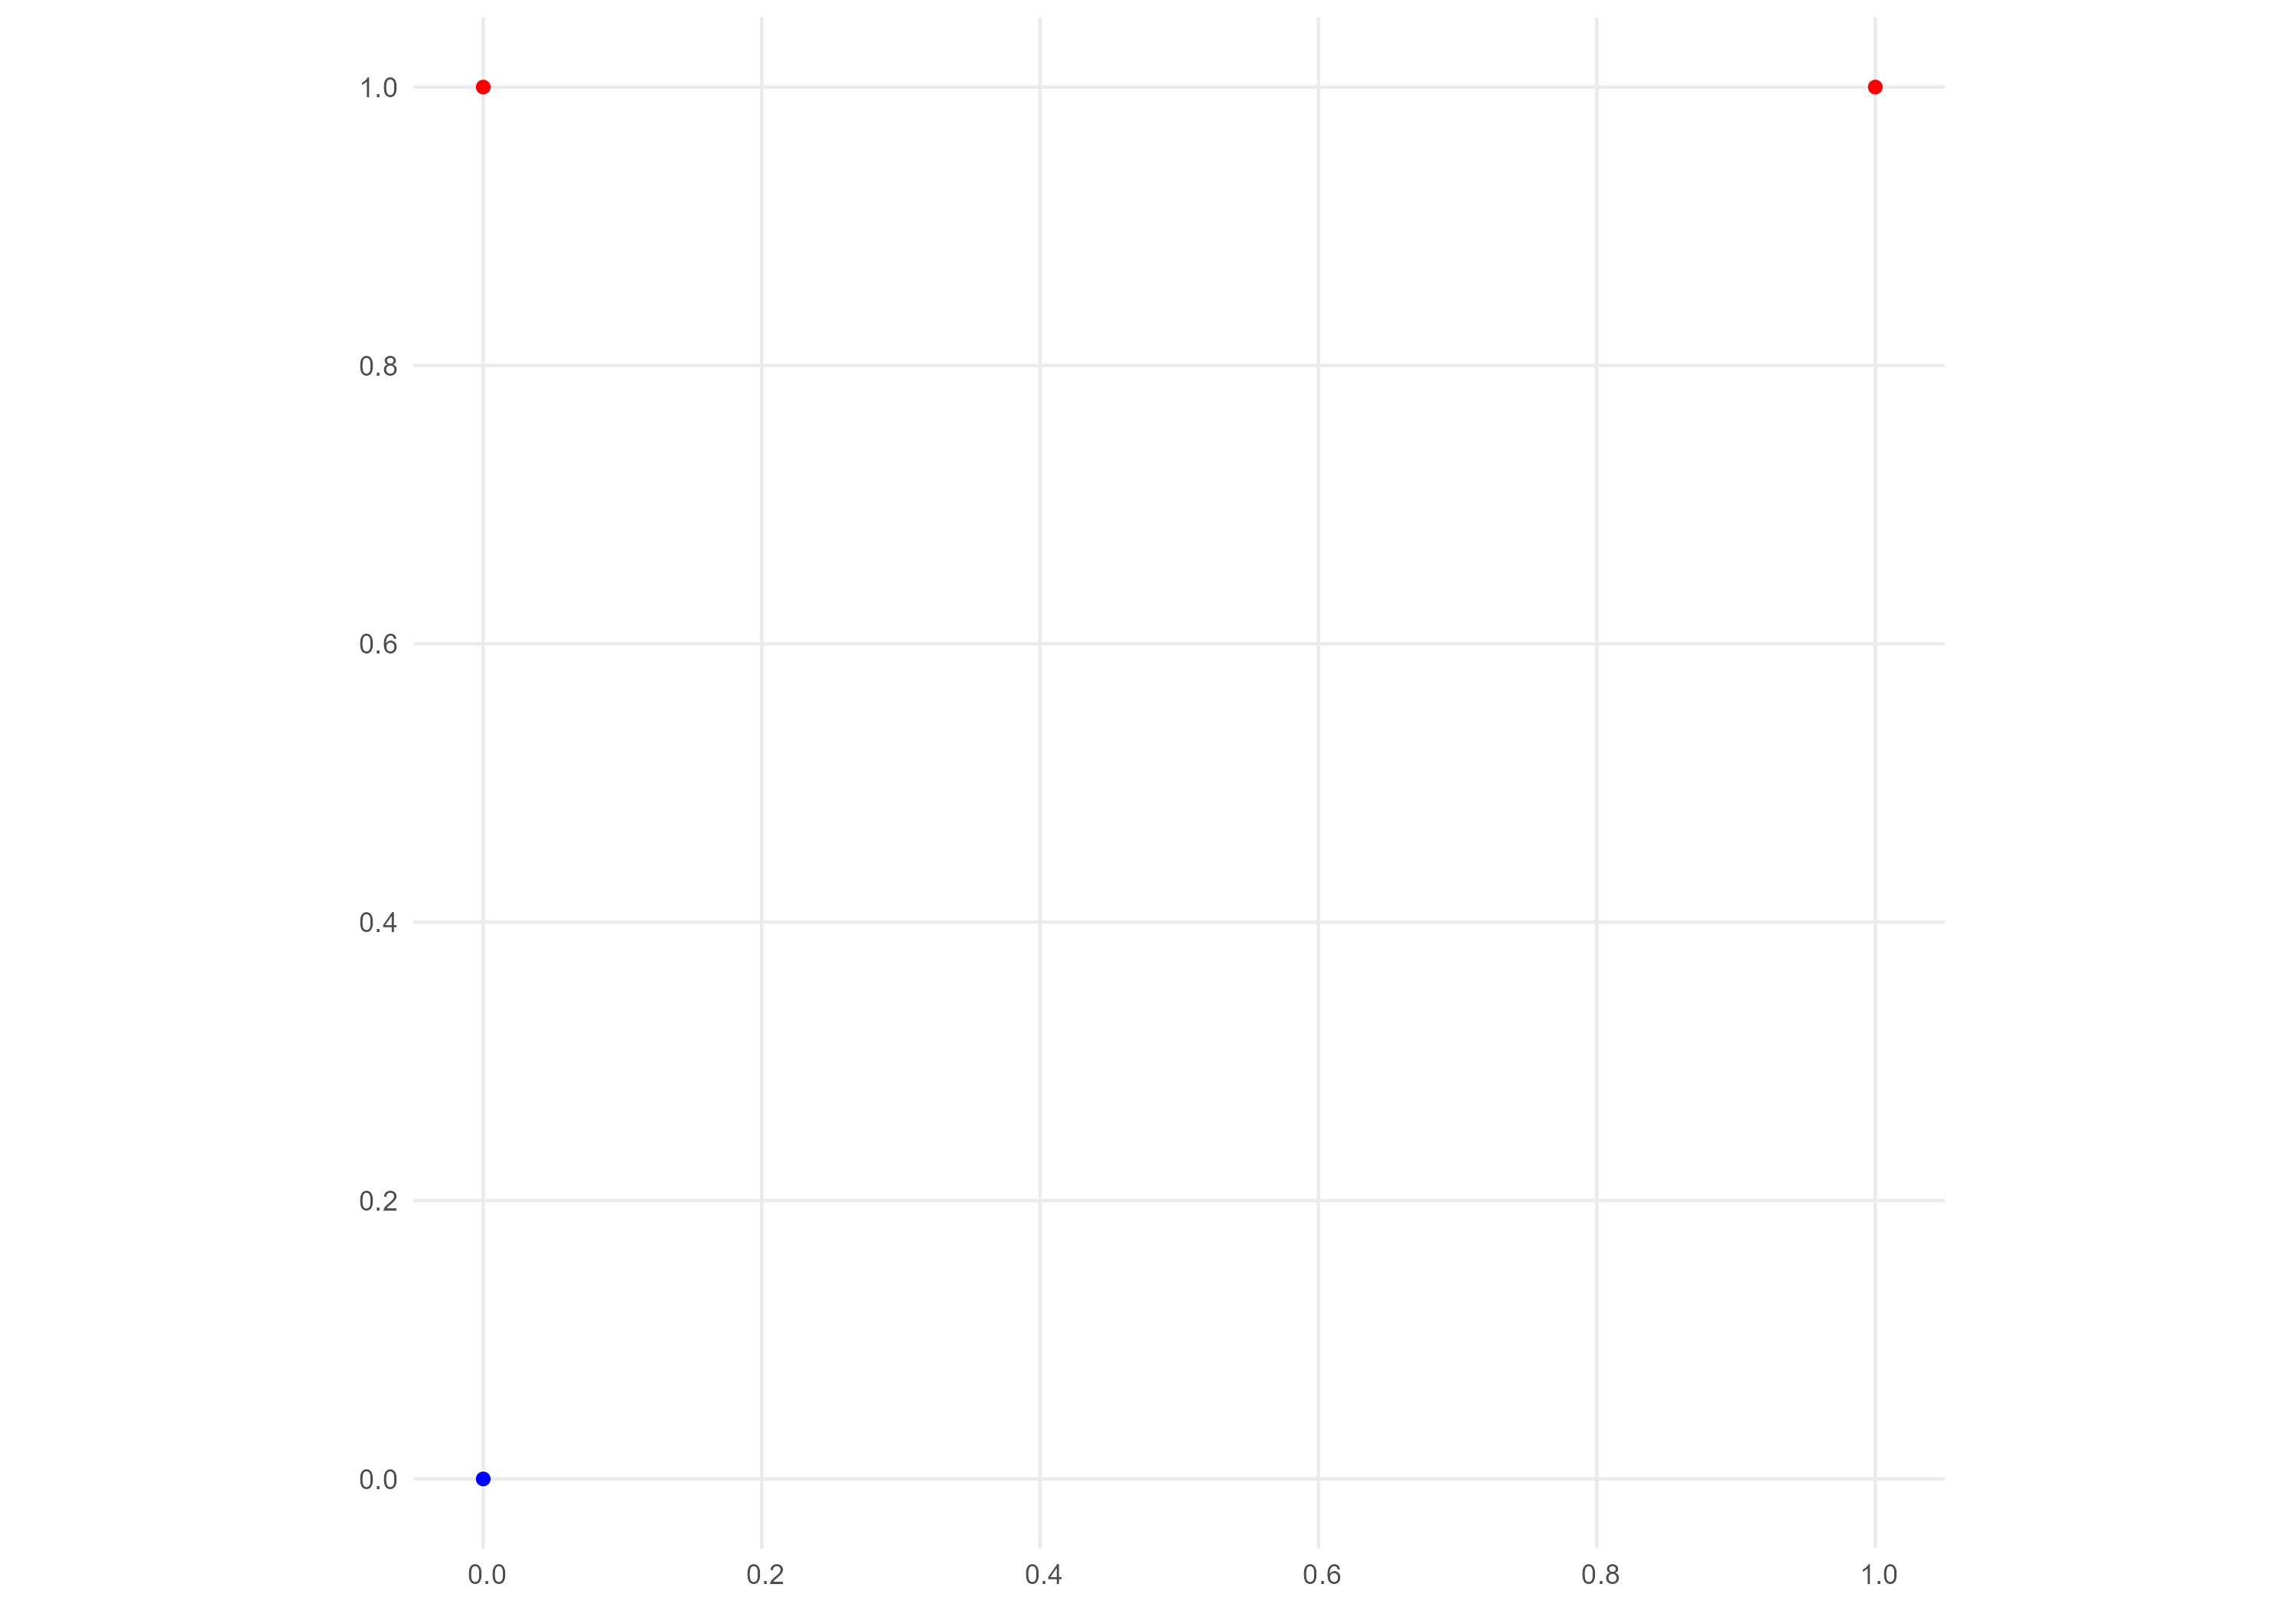
\includegraphics[width=1\textwidth]{figure/points.png}
	\end{figure}
\end{center}
\end{frame}



\begin{frame}[fragile]{Spatial Data}{Lines}
\begin{lstlisting}
m1 <- rbind(c(1, 1), c(2, 2), c(0.5, 0))
m2 <- rbind(c(2, 3), c(4, 4), c(3, 5))
m3 <- rbind(c(2, 4), c(1, 2))

one_l   <- st_linestring(m1)
multi_l <- st_multilinestring(list(m2, m3))
\end{lstlisting}
\begin{itemize}
	\item \texttt{m1} is defined as a matrix containing three coordinate pairs: (1, 1), (2, 2), and (0.5, 0). 
		\vspace{0.2cm}
	\begin{itemize}
	\item \texttt{m2} and \texttt{m3} are defined in the similar way	
				\vspace{0.2cm}
		\end{itemize}	
	\item \textbf{st\_linestring(m1)} creates a single spatial linestring object using the coordinates in \texttt{m1}.
		\vspace{0.2cm}
	\item \textbf{st\_multilinestring(list(m2, m3))} creates a multilinestring geometry by combining two linestrings defined in \texttt{m2} and \texttt{m3}.
\end{itemize}
\end{frame}



\begin{frame}[fragile]{Spatial Data}{Lines}
\begin{center}
	\begin{figure}[p]
		\centering
		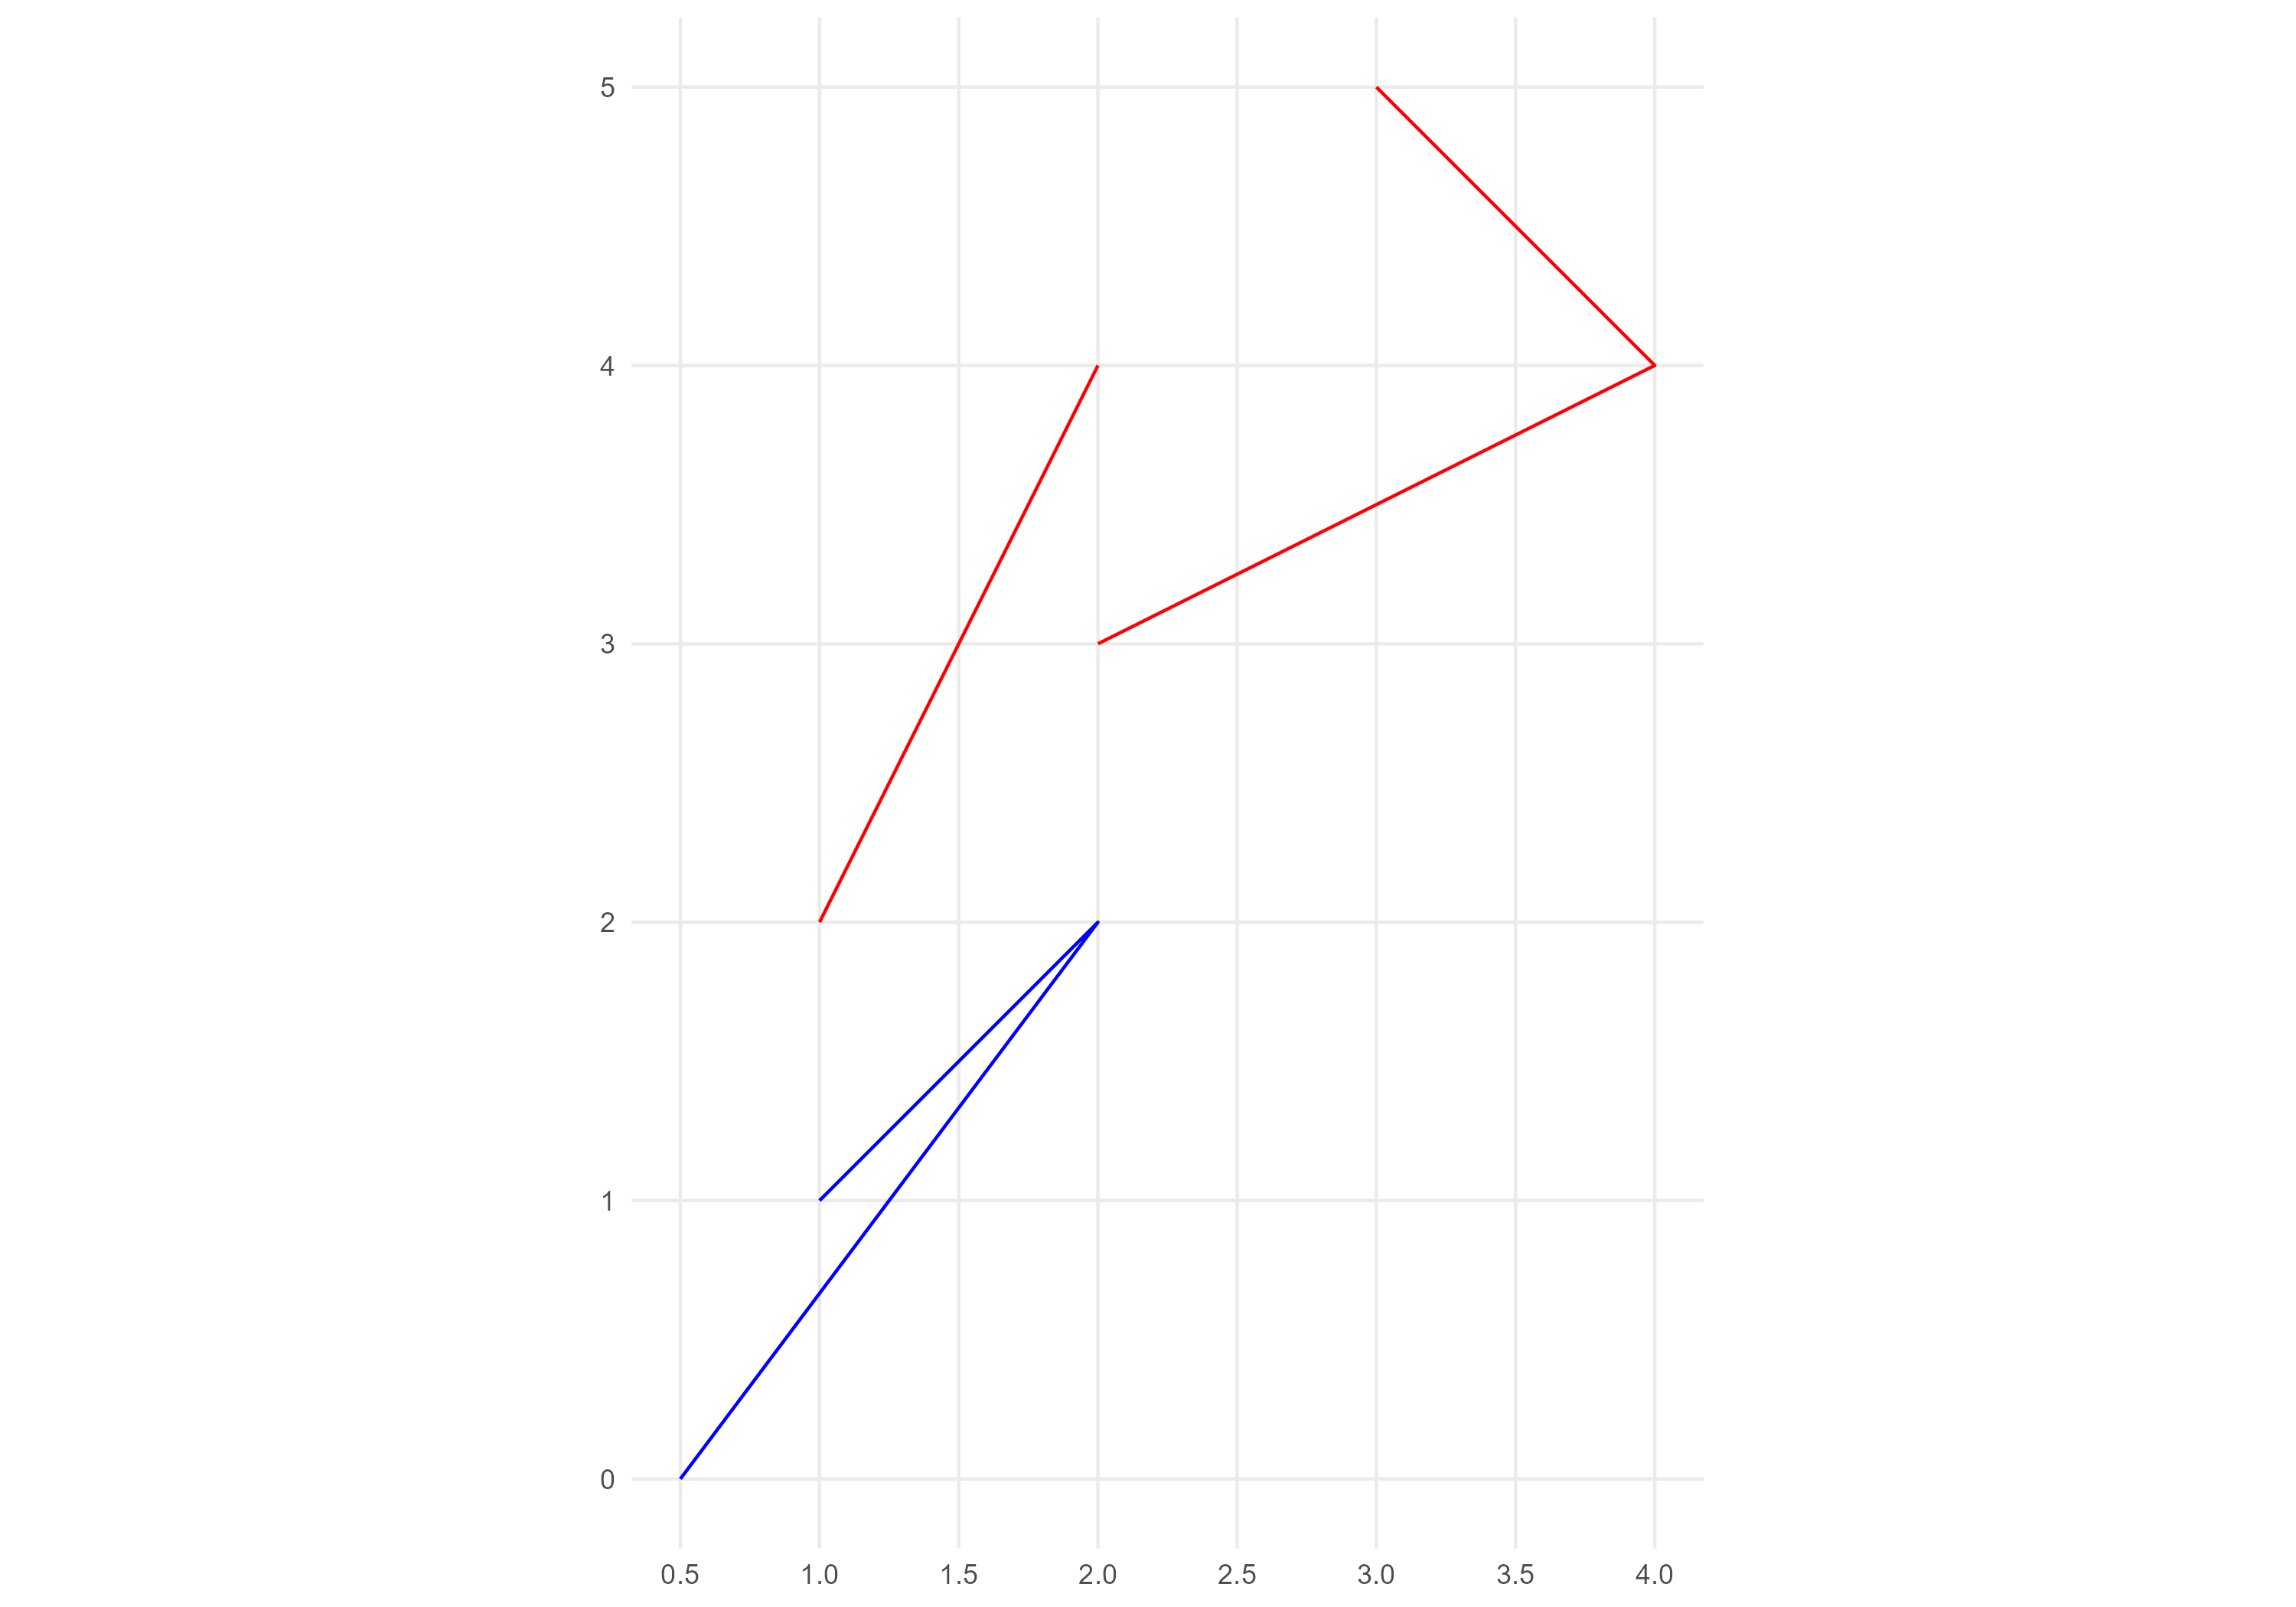
\includegraphics[width=1\textwidth]{figure/lines.png}
	\end{figure}
\end{center}
\end{frame}

\begin{frame}[fragile]{Spatial Data}{Polygons}
\begin{lstlisting}
m1 <- rbind(c(0, 0), c(2.5, 0), c(2, 2.5), c(0, 2.5), c(0, 0))
m2 <- rbind(c(1, 2), c(3, 3), c(3, 4), c(1, 2))
m3 <- rbind(c(2, 0), c(3, 1), c(2, 1), c(2, 0))

one_pol   <- st_polygon(list(m1))
multi_pol <- st_multipolygon(list(list(m2), list(m3)))
\end{lstlisting}
\begin{itemize}
	\item \texttt{m1} is defined as a matrix containing five coordinate pairs that form a closed polygon: (0, 0), (2.5, 0), (2, 2.5), (0, 2.5), and (0, 0).
	\vspace{0.2cm}
	\item \textbf{st\_polygon(list(m1))} creates a single spatial polygon object using the coordinates in \texttt{m1}.
	\vspace{0.2cm}
	\item \textbf{st\_multipolygon(list(list(m2), list(m3)))} creates a multipolygon geometry by combining two polygons defined in \texttt{m2} and \texttt{m3}.
\end{itemize}
\end{frame}



\begin{frame}[fragile]{Spatial Data}{Polygons}
\begin{center}
	\begin{figure}[p]
		\centering
		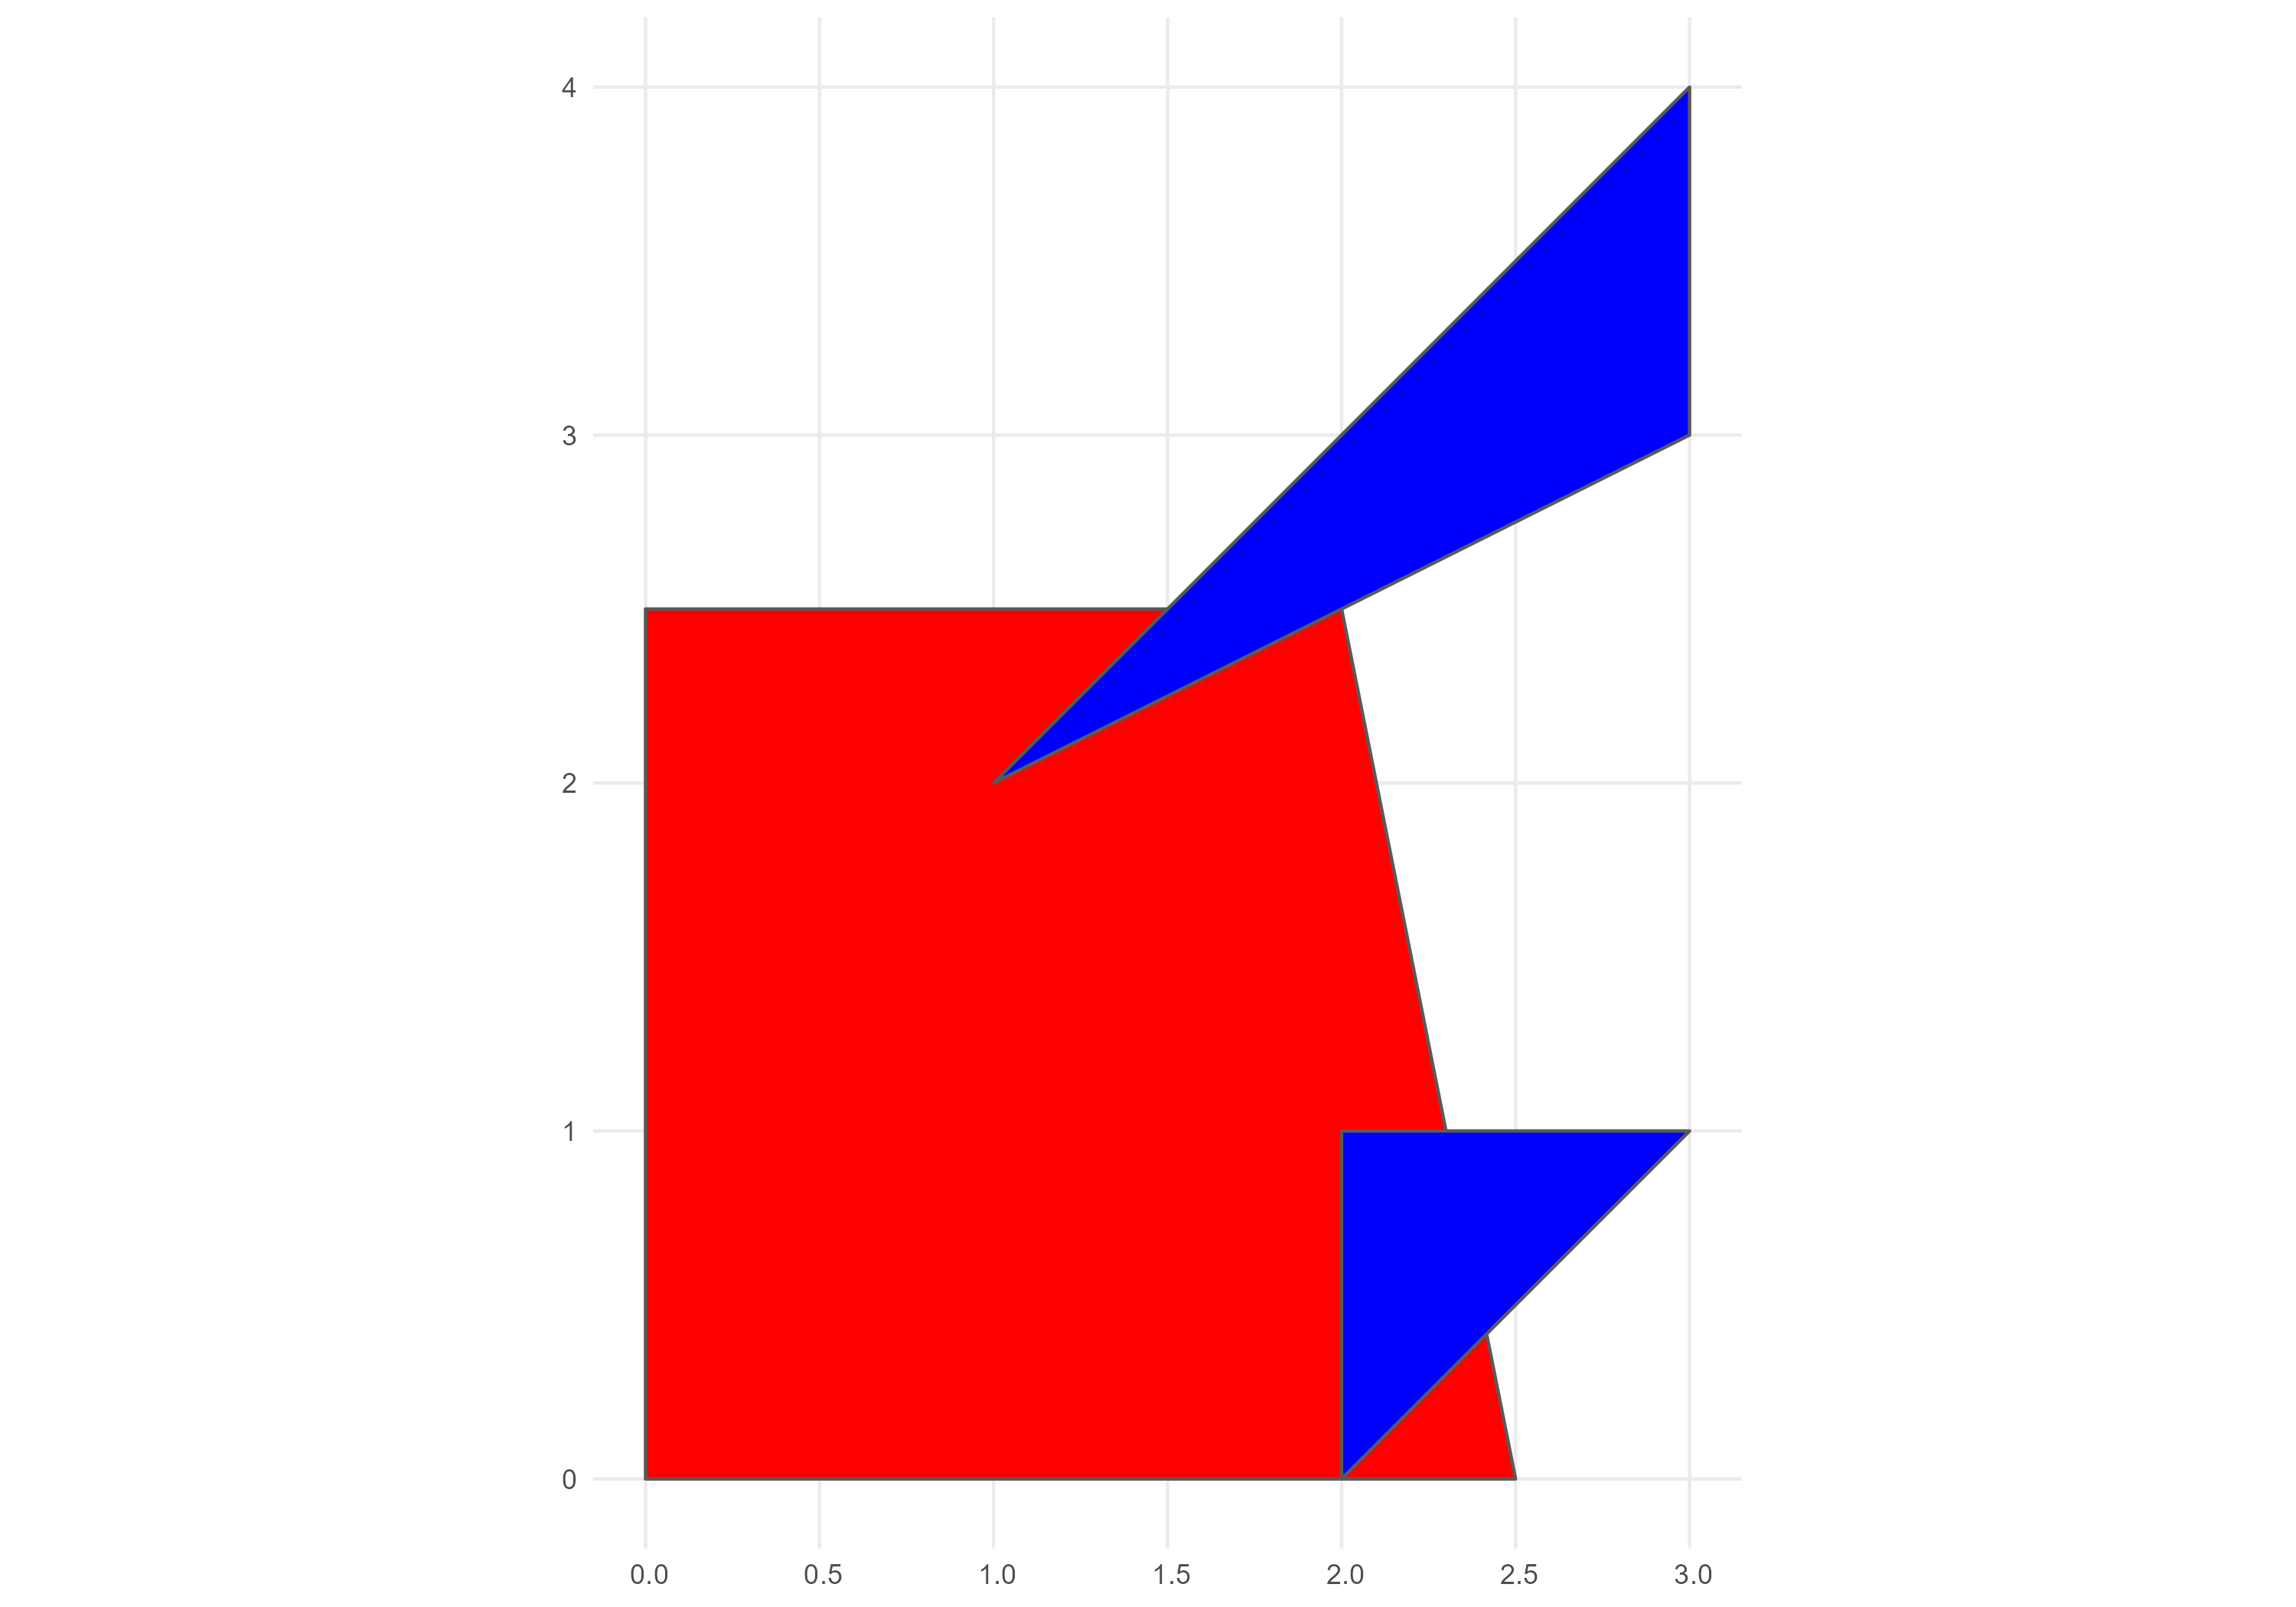
\includegraphics[width=1\textwidth]{figure/polygons.png}
	\end{figure}
\end{center}
\end{frame}





\begin{frame}[fragile]{Spatial Data}{Polygons}
\begin{lstlisting}
data_sfc <- st_sfc(one_p, multi_p,
one_l, multi_l,
one_pol, multi_pol)

class(data_sfc)
\end{lstlisting}
\begin{itemize}
	\item \texttt{m1} is defined as a matrix containing five coordinate pairs that form a closed polygon: (0, 0), (2.5, 0), (2, 2.5), (0, 2.5), and (0, 0).
	\vspace{0.2cm}
	\item \textbf{st\_polygon(list(m1))} creates a single spatial polygon object using the coordinates in \texttt{m1}.
	\vspace{0.2cm}
	\item \textbf{st\_multipolygon(list(list(m2), list(m3)))} creates a multipolygon geometry by combining two polygons defined in \texttt{m2} and \texttt{m3}.
\end{itemize}
\end{frame}




\begin{frame}[fragile]{Spatial Features Collection}{Polygons}
\begin{lstlisting}
data_sfc <- st_sfc(one_p, multi_p, one_l, multi_l, one_pol, multi_pol)
\end{lstlisting}
\begin{itemize}
	\item \textbf{st\_sfc} function combines various spatial objects, including points, linestrings, and polygons.
	\vspace{0.2cm}
	\begin{itemize}
	\item This is called a spatial features collection (SFC)
\end{itemize}
		\vspace{0.2cm}
	\item The `class(data\_sfc)` command is used to determine the class or data type of the resulting spatial features collection.
\end{itemize}
\end{frame}




\begin{frame}[fragile]{Creating a Spatial Data Frame}{}
\begin{lstlisting}
data_sf <- data.frame(name = c("A", "B", "C", "D", "E", "F"),
geometry = data_sfc)

data_sf <- st_sf(data_sf, geometry = data_sf$geometry)
\end{lstlisting}
\begin{itemize}
	\item The code begins by creating a data frame called `data\_sf`, which has two columns: `name` and `geometry`.
	\vspace{0.2cm}
	\item The \textbf{st\_sf} function is used to convert the data frame `data\_sf` into a spatial data frame (sf) 
		\vspace{0.2cm}
	\begin{itemize}
	\item Specifying the `geometry` column. 
		\vspace{0.2cm}
	\item This step associates the geometrical information with the data frame, making it suitable for spatial analysis.
\end{itemize}
\end{itemize}
\end{frame}



\title[]  
{Read and Save Spatial Data}


\author 
{}

%\institute{Institute of Economics, Academia Sinica  \\ Econ, NTU}
%\institute{Institute of Economics, Academia Sinica  \\ IMES/IDAS, NCCU}
\institute{}

%\author 
%{楊子霆 \\ 中研院經濟所}

%\institute 
%{中正大學國際經濟專題研討}




\date
{}


\begin{frame}{}
\titlepage
\end{frame}



\begin{frame}{Shapefile}
\begin{itemize}
	\item A Shapefile is a common file format for storing spatial data 
				\vspace{0.2cm}
				\begin{itemize}
	\item It was developed by Environmental Systems Research Institute (Esri)
						\vspace{0.2cm}
	\item A leading provider of GIS software and geodatabase management tools.
\end{itemize}
					\vspace{0.2cm}
		\item Shapefiles are widely supported by GIS software, making them a versatile and interoperable choice for sharing spatial data.
							\vspace{0.2cm}	
		\item They can represent various vector-based geographic elements, such as points, lines, and polygons.
		\vspace{0.2cm}			
	\item Shapefiles consist of a set of files with the same base name but different extensions

	

\end{itemize}
\end{frame}





\begin{frame}{Shapefile}


\begin{itemize}
	\item \textbf{.shp}: Record the actual coordinates of points, lines, and polygons.
			\vspace{0.2cm}
	\item \textbf{.shx}: Constructing a spatial index for geometric elements to improve search efficiency.
			\vspace{0.2cm}
	\item \textbf{.dbf}: Record the attribute data of geometric elements.
			\vspace{0.2cm}
	\item \textbf{.prj}: Store the projection information of geographic coordinate systems.
\end{itemize}


	\begin{center}
	\begin{figure}[p]
		\centering
		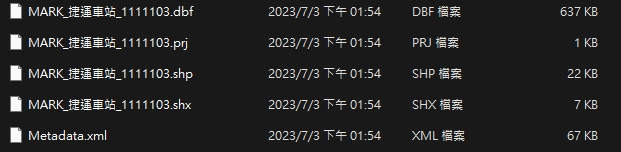
\includegraphics[width=.8\textwidth]{figure/捷運車站檔案.jpg}
	\end{figure}
\end{center}
\end{frame}






\begin{frame}[fragile]{Read a Shapefile}{Polygon}

\begin{lstlisting}
town <- st_read(dsn = str_c(path, "G97_A_CALIN_P.shp"), options = "ENCODING=UTF-8")

town <- read_sf(str_c(path, "G97_A_CALIN_P.shp"))
\end{lstlisting}
\begin{itemize}
\item Both functions read spatial data
\vspace{0.2cm}
\item \textbf{st\_read} provides more in-depth control for advanced operations
\vspace{0.2cm}
\item \textbf{read\_sf} is designed for ease of use and simplicity


\end{itemize}

\end{frame}



\begin{frame}[fragile]{Read a Shapefile}{Polygon}
	
\begin{lstlisting}
town_select <- read_sf(str_c(path, "G97_A_CALIN_P.shp")) %>%
select(c("SECT_NAME", "LIE_CODE", "SDFNAME"))

head(town_select) 
\end{lstlisting}
	\begin{itemize}
		\item \textbf{select()}: Only select specific columns (variables) in the spatial dataset
		\vspace{0.2cm}
		\item \textbf{head()}: show the variables in object \textbf{town\_select}
		
	\end{itemize}
	
\end{frame}



\begin{frame}[fragile]{Read a Shapefile}{Output}

\tiny

\begin{lstlisting}
Simple feature collection with 6 features and 3 fields
Geometry type: MULTIPOLYGON
Dimension:     XY
Bounding box:  xmin: 302583.4 ymin: 2784374 xmax: 308861.6 ymax: 2789176
CRS:           NA
# A tibble: 6 $\times$ 4
SECT_NAME LIE_CODE   SDFNAME                              geometry
<chr>     <chr>      <chr>                          <MULTIPOLYGON>
1 北投區    6301200042 湖田里10鄰 (((304697.5 2786869, 304692.4 278\ldots{}
2 士林區    6301100047 菁山里10鄰 (((307802.2 2787373, 307831.9 278\ldots{}
3 北投區    6301200042 湖田里9鄰  (((303166.5 2786151, 303171.5 278\ldots{}
\end{lstlisting}

\end{frame}



\begin{frame}[fragile]{Read a Shapefile}{Polygon}

\begin{lstlisting}
st_geometry(town[1, ])[[1]][[1]]
\end{lstlisting}
\begin{itemize}

\item \textbf{st\_geometry()}: This function extracts the geometry component of a simple features object
	\vspace{0.2cm}
\begin{itemize}
\item From the spatial object \textbf{town}, take the geometry of the first feature. Then, from that geometry, access its first primary component
\end{itemize}

\end{itemize}
\end{frame}


\begin{frame}[fragile]{Read a Shape File}{Output}


\begin{lstlisting}
[[1]]
[,1]    [,2]
[1,] 304697.5 2786869
[2,] 304692.4 2786880
[3,] 304701.6 2786928
[4,] 304697.1 2786956
[5,] 304696.7 2786978
[6,] 304686.3 2787008
[7,] 304680.4 2787034
[8,] 304681.6 2787058
[9,] 304687.7 2787084
[10,] 304690.9 2787093
\end{lstlisting}

\end{frame}


\begin{frame}[fragile]{Project Spatial Data}{Code}
	
\begin{lstlisting}
st_crs(town)

st_crs(town) <- 3826 #TWD97 / TM2 zone 121
\end{lstlisting}
	\begin{itemize}
		\item \textbf{st\_crs()}: this function is used to get or set the Coordinate Reference System (CRS) of a spatial object in R
		\vspace{0.2cm}
		\begin{itemize}
			\item \textbf{3826} refers to the TWD97 / TM2 zone 121 coordinate system, which is often used for spatial data in Taiwan
			
		\end{itemize}
	\end{itemize}
	
	
	
	
\end{frame}



\begin{frame}[fragile]{Read a Shapefile}{Point}
	
\begin{lstlisting}
mrt_station <- read_sf(str_c(path, "MARK_捷運車站_1111103.shp"))
mrt_station <- mrt_station[grep("臺北", mrt_station$MARKNAME1), ]
mrt_station <- mrt_station[-grep("出入口", mrt_station$MARKNAME1), ] %>% select(c("MARKNAME1"))
\end{lstlisting}
	\begin{itemize}
		
		\item Load a shapefile (spatial data) named "MARK\_捷運車站\_1111103.shp" into an object named mrt\_station
		\vspace{0.2cm}
		\begin{itemize}
			\item \textbf{grep()}: filters this data to only keep stations that are located in "臺北" (Taipei)
					\vspace{0.2cm}
			\item \textbf{-grep()}: removes any stations that have "出入口" (entrance/exit) in their names.		
								\vspace{0.2cm}
			\item It selects only the "MARKNAME1" column for the filtered data.					
		\end{itemize}
		
	\end{itemize}
\end{frame}




\begin{frame}{WKT Format}
\begin{itemize}
	\item Well-Known Text (WKT) is a text-based format used to represent and exchange spatial data
			\vspace{0.2cm}
			\begin{itemize}
	\item It provides a standardized way to describe geometric shapes, such as points, lines, and polygons, using a human-readable syntax.
			\vspace{0.2cm}
	\item It consists of text strings that define the structure and coordinates of geometries, making it platform-independent and easy to understand.
\end{itemize}
\end{itemize}
\end{frame}


\begin{frame}{WKT Format}
\begin{center}
	\begin{figure}[p]
		\centering
		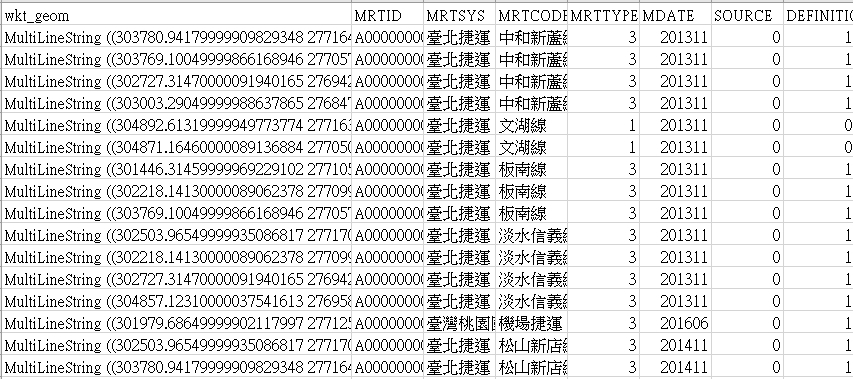
\includegraphics[width=1\textwidth]{figure/mrt_line.jpg}
	\end{figure}
\end{center}
\end{frame}

\begin{frame}[fragile]{Read CSV with WKT format}{Line}
\begin{lstlisting}
mrt_line <- read.csv(path_mrt_line) %>% 
filter(MRTSYS == "Taipei Metro", MRTCODE != "") 

mrt_line <- st_as_sf(mrt_line, wkt = c("wkt_geom"), crs = 3826)
\end{lstlisting}
\begin{itemize}
	\item This code reads a CSV file into a data frame.
	\vspace{0.2cm}
	\begin{itemize}
		\item It then filters the data to select only rows where the "MRTSYS" column equals "Taipei Metro" and the "MRTCODE" column is not empty.
	\end{itemize}
	\vspace{0.2cm}
	\item \textbf{st\_as\_sf()} function converts the data frame into a spatial data frame (sf).
	\vspace{0.2cm}
	\begin{itemize}
		\item The `wkt` argument specifies the name of the column containing Well-Known Text (WKT) format geometries
			\vspace{0.2cm}
		\item The `crs` argument sets the coordinate reference system (CRS) to 3826.
	\end{itemize}
\end{itemize}
\end{frame}





\begin{frame}[fragile]{Read CSV with Coordinates}{Point}
\begin{lstlisting}
house <- read.csv(path_house) %>% 
select(c("h_price_m2", "address", "latitude", "longitude"))

house <- st_as_sf(house, coords = c("longitude", "latitude"), 
crs = 3826)
\end{lstlisting}
\begin{itemize}
	
	\item  `\textbf{st\_as\_sf()}` function convert the data frame into a spatial data frame (sf).
	\vspace{0.2cm}
	\begin{itemize}
		\item The `coords` argument specifies the columns that contain the latitude and longitude coordinates, which are "longitude" and "latitude" in this case.
			\vspace{0.2cm}
		\item The `crs` argument sets the coordinate reference system (CRS) to 3826.
	\end{itemize}
\end{itemize}
\end{frame}








\begin{frame}[fragile]{Combine All Spatial Objects}{Graph}
	
\begin{lstlisting}
p<-ggplot() + 
geom_sf(data = town) +
geom_sf(data = mrt_line, color = "red", size = 1) +
geom_sf(data = mrt_station, color = "red", size = 1) +
theme_minimal()

ggsave(filename = str_c(path,"tpe_mrt.png"), plot = p, width = 10, height = 7)
\end{lstlisting}
	\begin{itemize}
		
		\item This code combines multiple spatial objects in a single graph using the `ggplot2` package
		\vspace{0.2cm}
		\begin{itemize}
			\item `\textbf{geom\_sf}` layers are added to the plot to display different spatial objects, including "town," "mrt\_line," and "mrt\_station."				
		\end{itemize}
		
	\end{itemize}
\end{frame}




\begin{frame}[fragile]{Combine All Spatial Objects}{MRT Line in Taipei}
\begin{center}
	\begin{figure}[p]
		\centering
		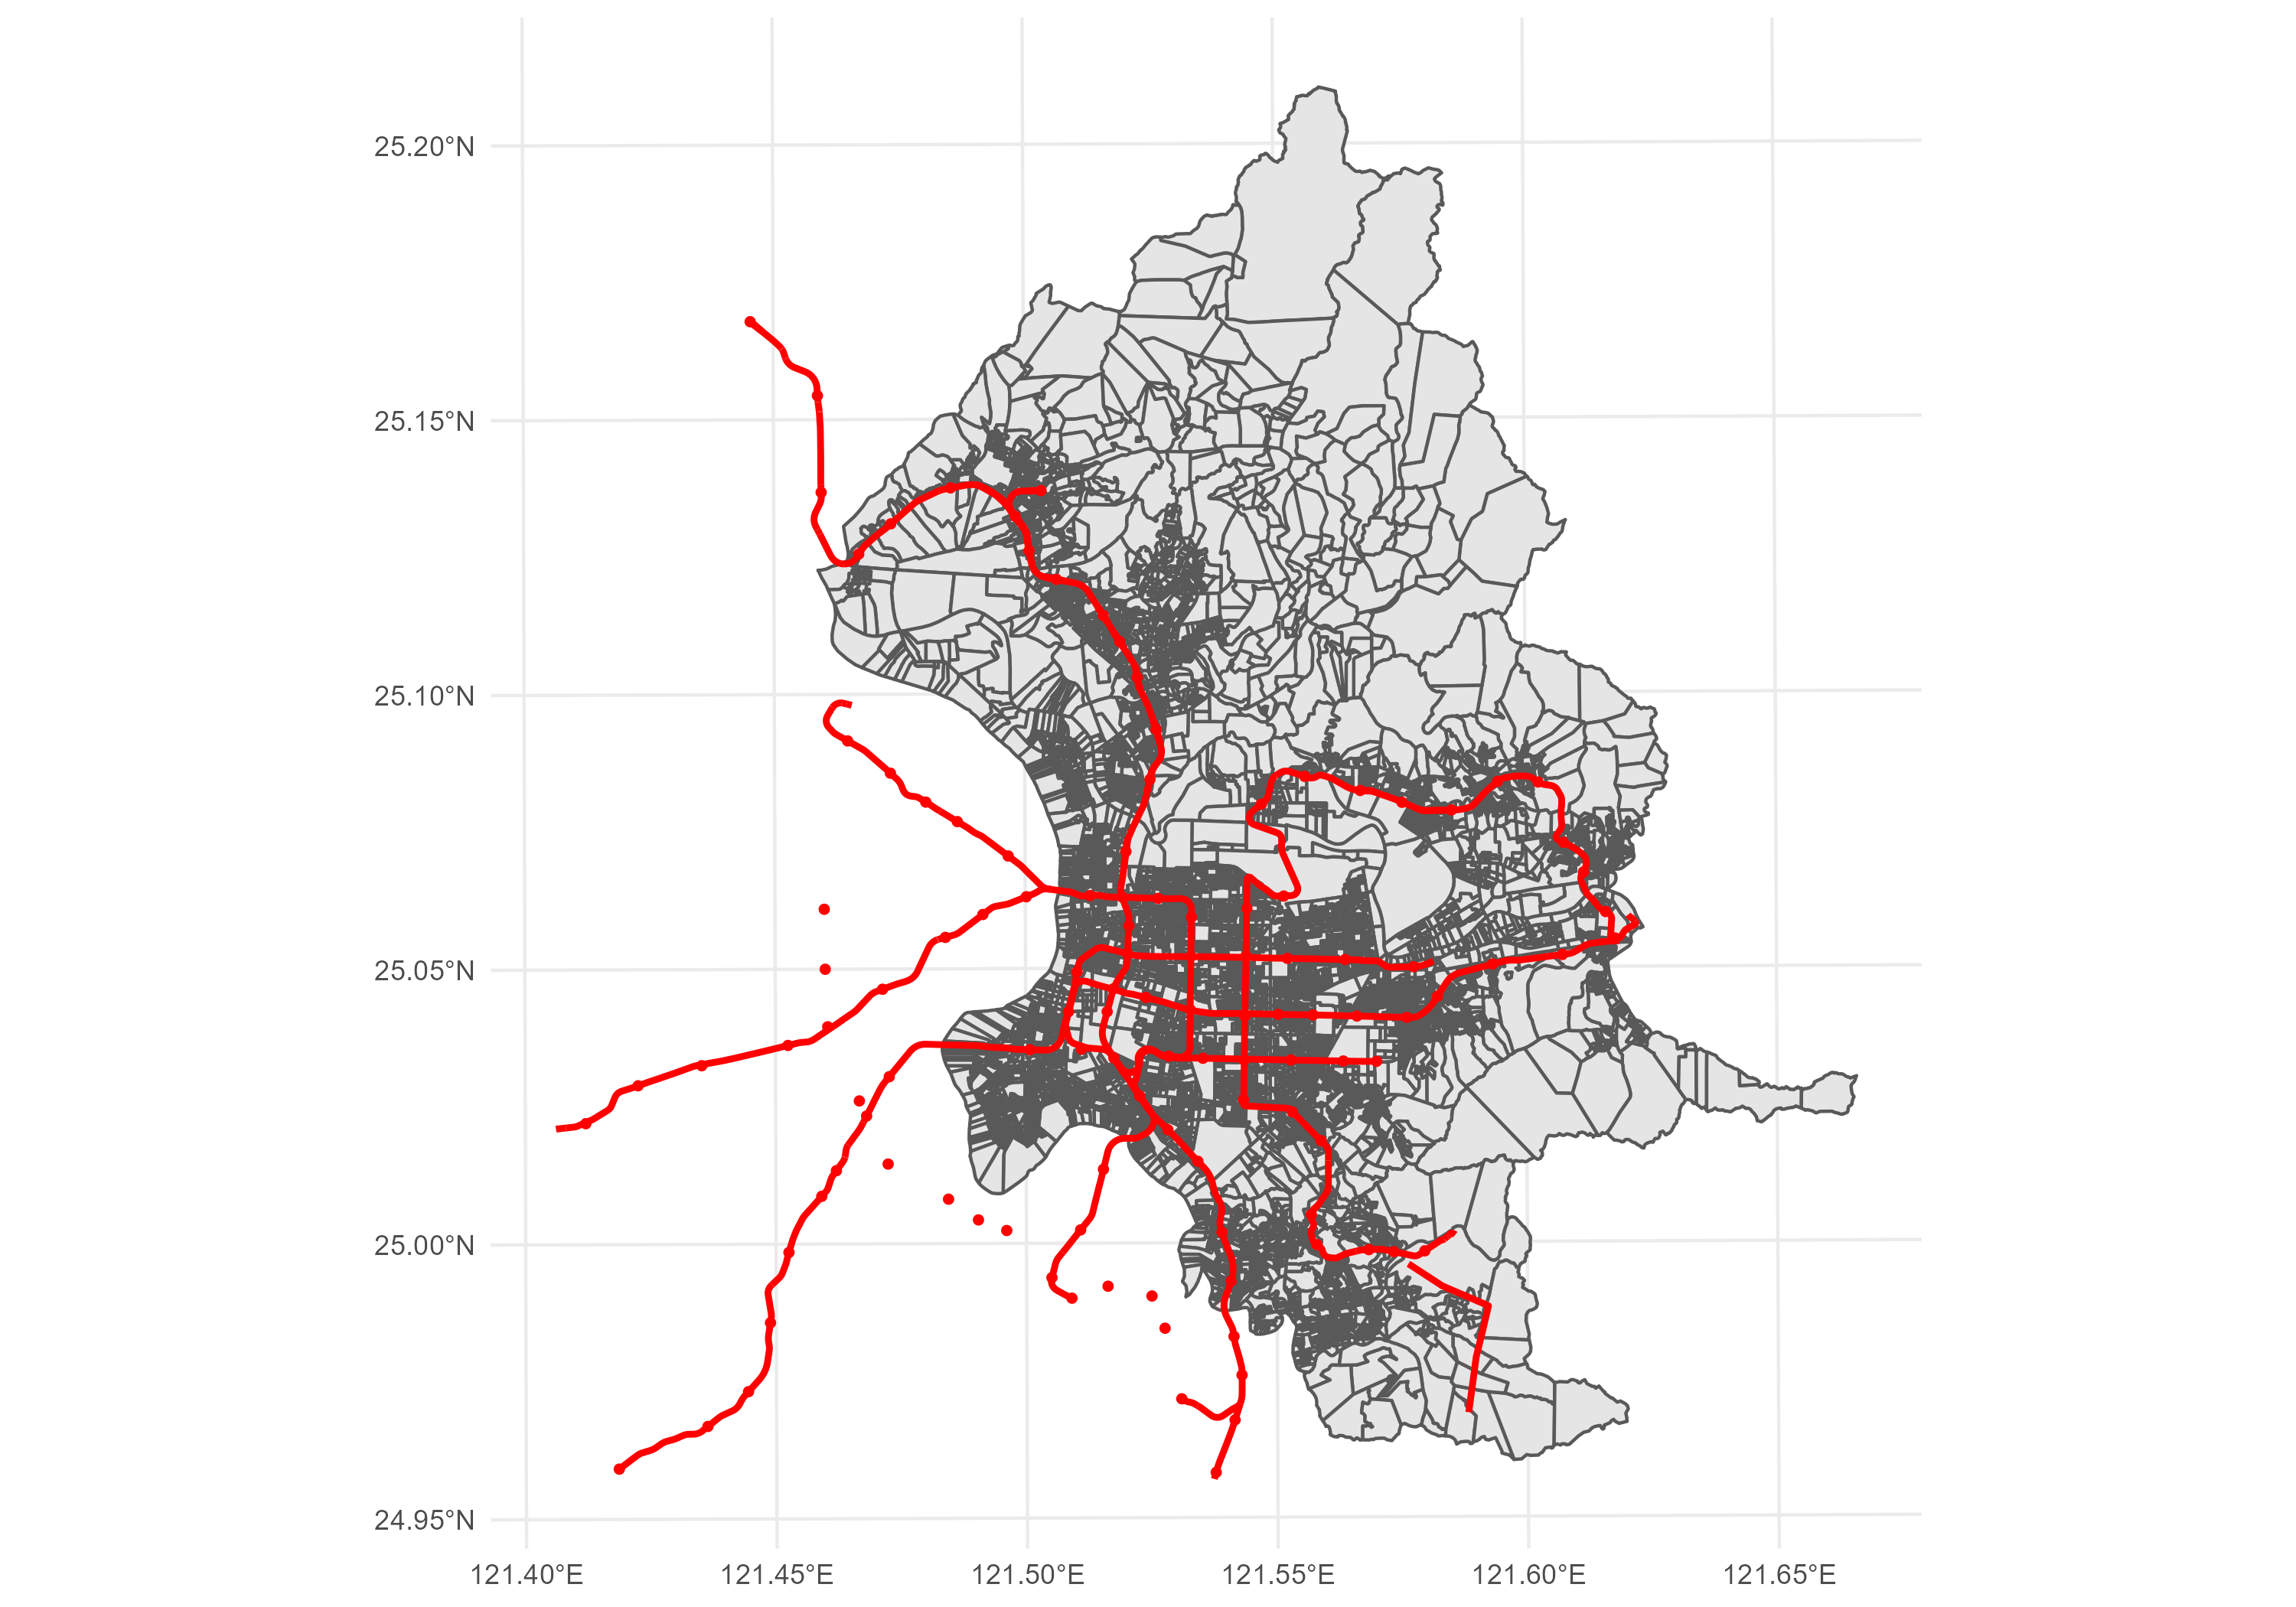
\includegraphics[width=1\textwidth]{figure/tpe_mrt.png}
	\end{figure}
\end{center}
\end{frame}

\begin{frame}[fragile]{Re-project Spatial Data}
	\begin{itemize}
		
	\item Sometimes we might have spatial data in different coordinate systems
				\vspace{0.2cm}
		\begin{itemize}
			\item \textbf{WGS84:} latitude-longitude coordinate system		
						\vspace{0.2cm}
			\item \textbf{TWD97:} Taiwan Transverse Mercator coordinate system
		\end{itemize}
			\vspace{0.2cm}
		\item Therefore, it is necessary to convert them to the same coordinate system in order to perform data processing.
	\end{itemize}
\end{frame}


\begin{frame}[fragile]{Re-project Spatial Data}
\begin{lstlisting}
st_crs(house)$epsg #TWD97 / TM2 zone 121

house_4326 <- st_transform(house, crs = 4326) #WGS84
\end{lstlisting}
\begin{itemize}
	\item This code demonstrates the process of re-projecting spatial data
	\vspace{0.2cm}
	
		\item The `\textbf{st\_transform()}` function is used to re-project the `house` spatial data to a new CRS, which is specified as 4326 (WGS84), a commonly used geographic coordinate system.
		\vspace{0.2cm}
		\begin{itemize}
		\item The CRS of re-projected data is specified as 4326 (WGS84)
		\end{itemize}
	
		\end{itemize}
		\end{frame}

\begin{frame}[fragile]{Spatial Measurement -- Distance}{R Output}

\tiny

\begin{lstlisting}
Simple feature collection with 6 features and 2 fields
Geometry type: POINT
Dimension:     XY
Bounding box:  xmin: 121.5111 ymin: 24.98659 xmax: 121.6171 ymax: 25.14144
Geodetic CRS:  WGS 84
h_price_m2                                  address                  geometry
1     161451              台北市南港區興南街150號10樓 POINT (121.5987 25.05488)
2     261347 臺北市信義區安康里29鄰松勇路69巷10號17樓 POINT (121.5702 25.03316)
3     213985          臺北市內湖區康寧路三段187號七樓 POINT (121.6121 25.07005)
\end{lstlisting}


\end{frame}

\begin{frame}[fragile]{Save to a New Shapefile}
\begin{lstlisting}
write_sf(house, "house.shp")
\end{lstlisting}
\begin{itemize}
	\item \textbf{write\_sf()} function save spatial data to a new Shapefile format.
	\vspace{0.2cm}
	\begin{itemize}
		
		\item The second argument `"house.shp"` specifies the file name for the new Shapefile.
	\end{itemize}

\end{itemize}
\end{frame}


\begin{frame}[fragile]{Drawbacks of Shapefiles}
	\begin{itemize}
		
		\item Limited data storage:
		\vspace{0.2cm}
		\begin{itemize}
			\item Shapefiles have a maximum file size limit of 2GB and can store only up to 255 fields (attribute data)
			\vspace{0.2cm}
			\item Additionally, there is a restriction on attribute field names, which cannot exceed 10 characters
						\vspace{0.2cm}
			\item These limitations can pose constraints when working with large or complex datasets.
		\end{itemize}
	
	\end{itemize}
\end{frame}


\begin{frame}[fragile]{Drawbacks of Shapefiles}
	\begin{itemize}
		
		\item Inefficient data storage:
		\vspace{0.2cm}
		\begin{itemize}
			\item Shapefiles store data in a binary format, which can result in larger file sizes compared to other file formats
			\vspace{0.2cm}
			\item Increased storage requirements and slower data access
		\end{itemize}
		
	\end{itemize}
\end{frame}



\begin{frame}[fragile]{Alternatives -- Save as gpkg}
	\begin{itemize}
		
		\item For ArcGIS user, one of the alternative data formats  is GeoPackage. 
				\vspace{0.2cm}
		\item Unlike the shapefile system, it produces only a single file with .gpkg extension. 
				\vspace{0.2cm}
		\item Note that GeoPackage files can also be easily read into ArcGIS.
		
	
		
	\end{itemize}
\end{frame}



\begin{frame}[fragile]{Alternatives -- Save as GeoPackage (gpkg)}
\begin{lstlisting}
write_sf(house, "house.gpkg")
\end{lstlisting}
\begin{itemize}
	\item The \textbf{write\_sf()} function is used to save the `house` spatial data to a new GeoPackage file.
	\vspace{0.2cm}
	\begin{itemize}
		\item The file name `"house.gpkg"` is specified with the `.gpkg` extension, which is commonly used for GeoPackages.
	\end{itemize}
\end{itemize}

\begin{lstlisting}
house_gpkg <- read_sf("house.gpkg")
\end{lstlisting}
\begin{itemize}
	\item \textbf{read\_sf()} function reads the saved GeoPackage file `"house.gpkg"` back into a new spatial data frame
\end{itemize}
\end{frame}





\begin{frame}[fragile]{Alternatives -- Save as RDS}
	\begin{itemize}
		
		\item For R user, one of the alternative data formats  is  rds file
		\vspace{0.2cm}
		\item The use of rds files can be particularly attractive when the dataset is large 
		\vspace{0.2cm}
		\item Because rds files are typically more memory efficient than shapefiles, eating up less of your disk memory.
		
		
	\end{itemize}
\end{frame}



\begin{frame}[fragile]{Alternatives -- Save as RDS (R Data)
}
\begin{lstlisting}
saveRDS(house, "house.rds")
\end{lstlisting}
\begin{itemize}
	\item The \textbf{saveRDS()} function is used to save the `house` spatial data to a new RDS file.
	\vspace{0.2cm}
	\begin{itemize}
		\item The file name `"house.rds"` is specified with the `.rds` extension, which is commonly used for R Data files.
	\end{itemize}
\end{itemize}

\begin{lstlisting}
house_rds <- readRDS("house.rds")
\end{lstlisting}
\begin{itemize}
	\item \textbf{readRDS()} reads the saved RDS file `"house.rds"` back into a new object called `house\_rds`
\end{itemize}
\end{frame}





\title[]  
{Spatial Operations}


\author 
{}

%\institute{Institute of Economics, Academia Sinica  \\ Econ, NTU}
%\institute{Institute of Economics, Academia Sinica  \\ IMES/IDAS, NCCU}
\institute{}

%\author 
%{楊子霆 \\ 中研院經濟所}

%\institute 
%{中正大學國際經濟專題研討}




\date
{}


\begin{frame}{}
	\titlepage
\end{frame}



\begin{frame}{Spatial Join}{Overview}
	\begin{itemize}
		\item Using geographic location to combine two spatial datasets 
				\vspace{0.2cm}
		\begin{itemize}
	\item Combines attributes from one layer to another based on this geographic relationship
					\vspace{0.2cm}
	\item E.g., determining which address points (from one dataset) are within which neighborhoods (from another dataset)			
				\end{itemize}	
				
				
	\end{itemize}
\end{frame}



\begin{frame}{Spatial Join}{Different Types Based on Relationships}

	\begin{itemize}
		\item \textbf{Intersect:} Features that overlap or share space
							\vspace{0.2cm}
		\item \textbf{Within:} One feature geographically contained within another
							\vspace{0.2cm}
		\item \textbf{Contains:} Opposite of "within" - one feature encloses another
							\vspace{0.2cm}
		\item \textbf{Closest:} Joining features based on proximity
	\end{itemize}
\end{frame}

\begin{frame}{Spatial Joins}{Applications}
	\begin{itemize}
		\item Results used for various types of spatial analysis
									\vspace{0.2cm}
		\item Determining density, proximity, or percentage of certain characteristics
									\vspace{0.2cm}
		\item Analyzing number of facilities within regions, prevalence of factors near schools, etc.
	\end{itemize}
\end{frame}




\begin{frame}[fragile]{Spatial Joins}{R code}
\begin{lstlisting}
house_join <- st_join(house, town)
\end{lstlisting}
\begin{itemize}
	\item This code demonstrates a spatial join operation between two spatial data frames: `house` and `town`.
	\vspace{0.2cm}
	\item Both `house` and `town` contain spatial information, such as geometries (e.g., points or polygons).
	\vspace{0.2cm}
	\item The \textbf{st\_join()} function uses the "intersects" method, which means it joins the rows from `house` to `town` where the geometries intersect
	\vspace{0.2cm}
	\begin{itemize}
		\item Where they share any portion of space.
	\end{itemize}
\end{itemize}
\end{frame}




\begin{frame}[fragile]{Spatial Joins}{R Output}
	
	\tiny
	
\begin{lstlisting}
Simple feature collection with 6 features and 9 fields
Geometry type: POINT
Dimension:     XY
Bounding box:  xmin: 301535 ymin: 2764405 xmax: 312256 ymax: 2781542
Projected CRS: TWD97 / TM2 zone 121
h_price_m2                                  address
1     161451              台北市南港區興南街150號10樓
2     261347 臺北市信義區安康里29鄰松勇路69巷10號17樓
SECT_NAME SECT_CODE LIE_NAME   LIE_CODE LI_NO        SDFKEY
1    南港區   6300900   東新里 6300900005   019 6300900005019
2    信義區   6300200   安康里 6300200009   029 6300200009029
SDFNAME               geometry
1 東新里19鄰 POINT (310403 2771990)
2 安康里29鄰 POINT (307543 2769572)
\end{lstlisting}
	
\end{frame}








\begin{frame}{Spatial Aggregation}{Overview}
	
	\begin{itemize}
		\item Spatial aggregation is a common procedure in GIS
					\vspace{0.2cm}
			\begin{itemize}
		 \item Combining spatially located data into groups that share common geographic boundaries or characteristics
		 
		 	\end{itemize}
	
	\end{itemize}
\end{frame}

\begin{frame}{Spatial Aggregation}{Advantages}
	
	\begin{itemize}
		\item \textbf{Grouping by Geographical Boundaries:} Data points aggregated based on shared geographic areas.
							\vspace{0.2cm}
		\item \textbf{Reducing Complexity:} Simplifies spatial data, highlighting trends or patterns.
							\vspace{0.2cm}
		\item \textbf{Statistical Summarization:} Provides average or median values within geographical units.
	\end{itemize}
\end{frame}



\begin{frame}{Spatial Aggregation}{Challenges}	
	\begin{itemize}
		\item \textbf{Modifiable Areal Unit Problem (MAUP):} Different aggregation levels can lead to different analysis results
									\vspace{0.2cm}
			\begin{itemize}
		\item Importance of defining appropriate spatial boundaries for aggregation.
			\end{itemize}
	\end{itemize}
\end{frame}










\begin{frame}[fragile]{Spatial Aggregation}{R Output}
\begin{lstlisting}
district <- group_by(town, SECT_NAME) %>% summarise(count = n())
\end{lstlisting}
\begin{itemize}
	\item This code demonstrates a spatial aggregation operation on the `town` spatial data frame.
	\vspace{0.2cm}
	\item The \textbf{group\_by()} function is used to group the data by the `SECT\_NAME` variable (區名) within the `town` data frame.
	
	\begin{itemize}
		\vspace{0.2cm}
		\item The \textbf{summarise()} function calculates the count of features in each district 
	\end{itemize}
	
\end{itemize}
\end{frame}




\begin{frame}[fragile]{Spatial Aggregation}{R Output}
	
	\tiny
	
\begin{lstlisting}
Simple feature collection with 6 features and 2 fields
Geometry type: POLYGON
Dimension:     XY
Bounding box:  xmin: 296266.1 ymin: 2766795 xmax: 317197.3 ymax: 2789176
Projected CRS: TWD97 / TM2 zone 121
# A tibble: 6 $\times$ 3
SECT_NAME count                                     geometry
<chr>     <int>                                <POLYGON [m]>
1 中山區      877 ((303114 2771127, 303073.9 2771140, 303052.\ldots{}
2 中正區      582 ((302426.9 2768031, 302382.4 2768063, 30237\ldots{}
3 信義區      922 ((307636.1 2767150, 307636.2 2767129, 30763\ldots{}
\end{lstlisting}
	
\end{frame}



\begin{frame}[fragile]{Spatial Aggregation}{R Code}
	
\begin{lstlisting}
district_plot <- ggplot() + 
geom_sf(data = district, aes(fill = count), linetype = "blank") +
scale_fill_gradient(low = "lightblue", high = "darkblue")
\end{lstlisting}
	
\end{frame}




\begin{frame}{Spatial Aggregation}{Housing Transactions by Districts}{}
	\begin{center}
		\begin{figure}[p]
			\centering
			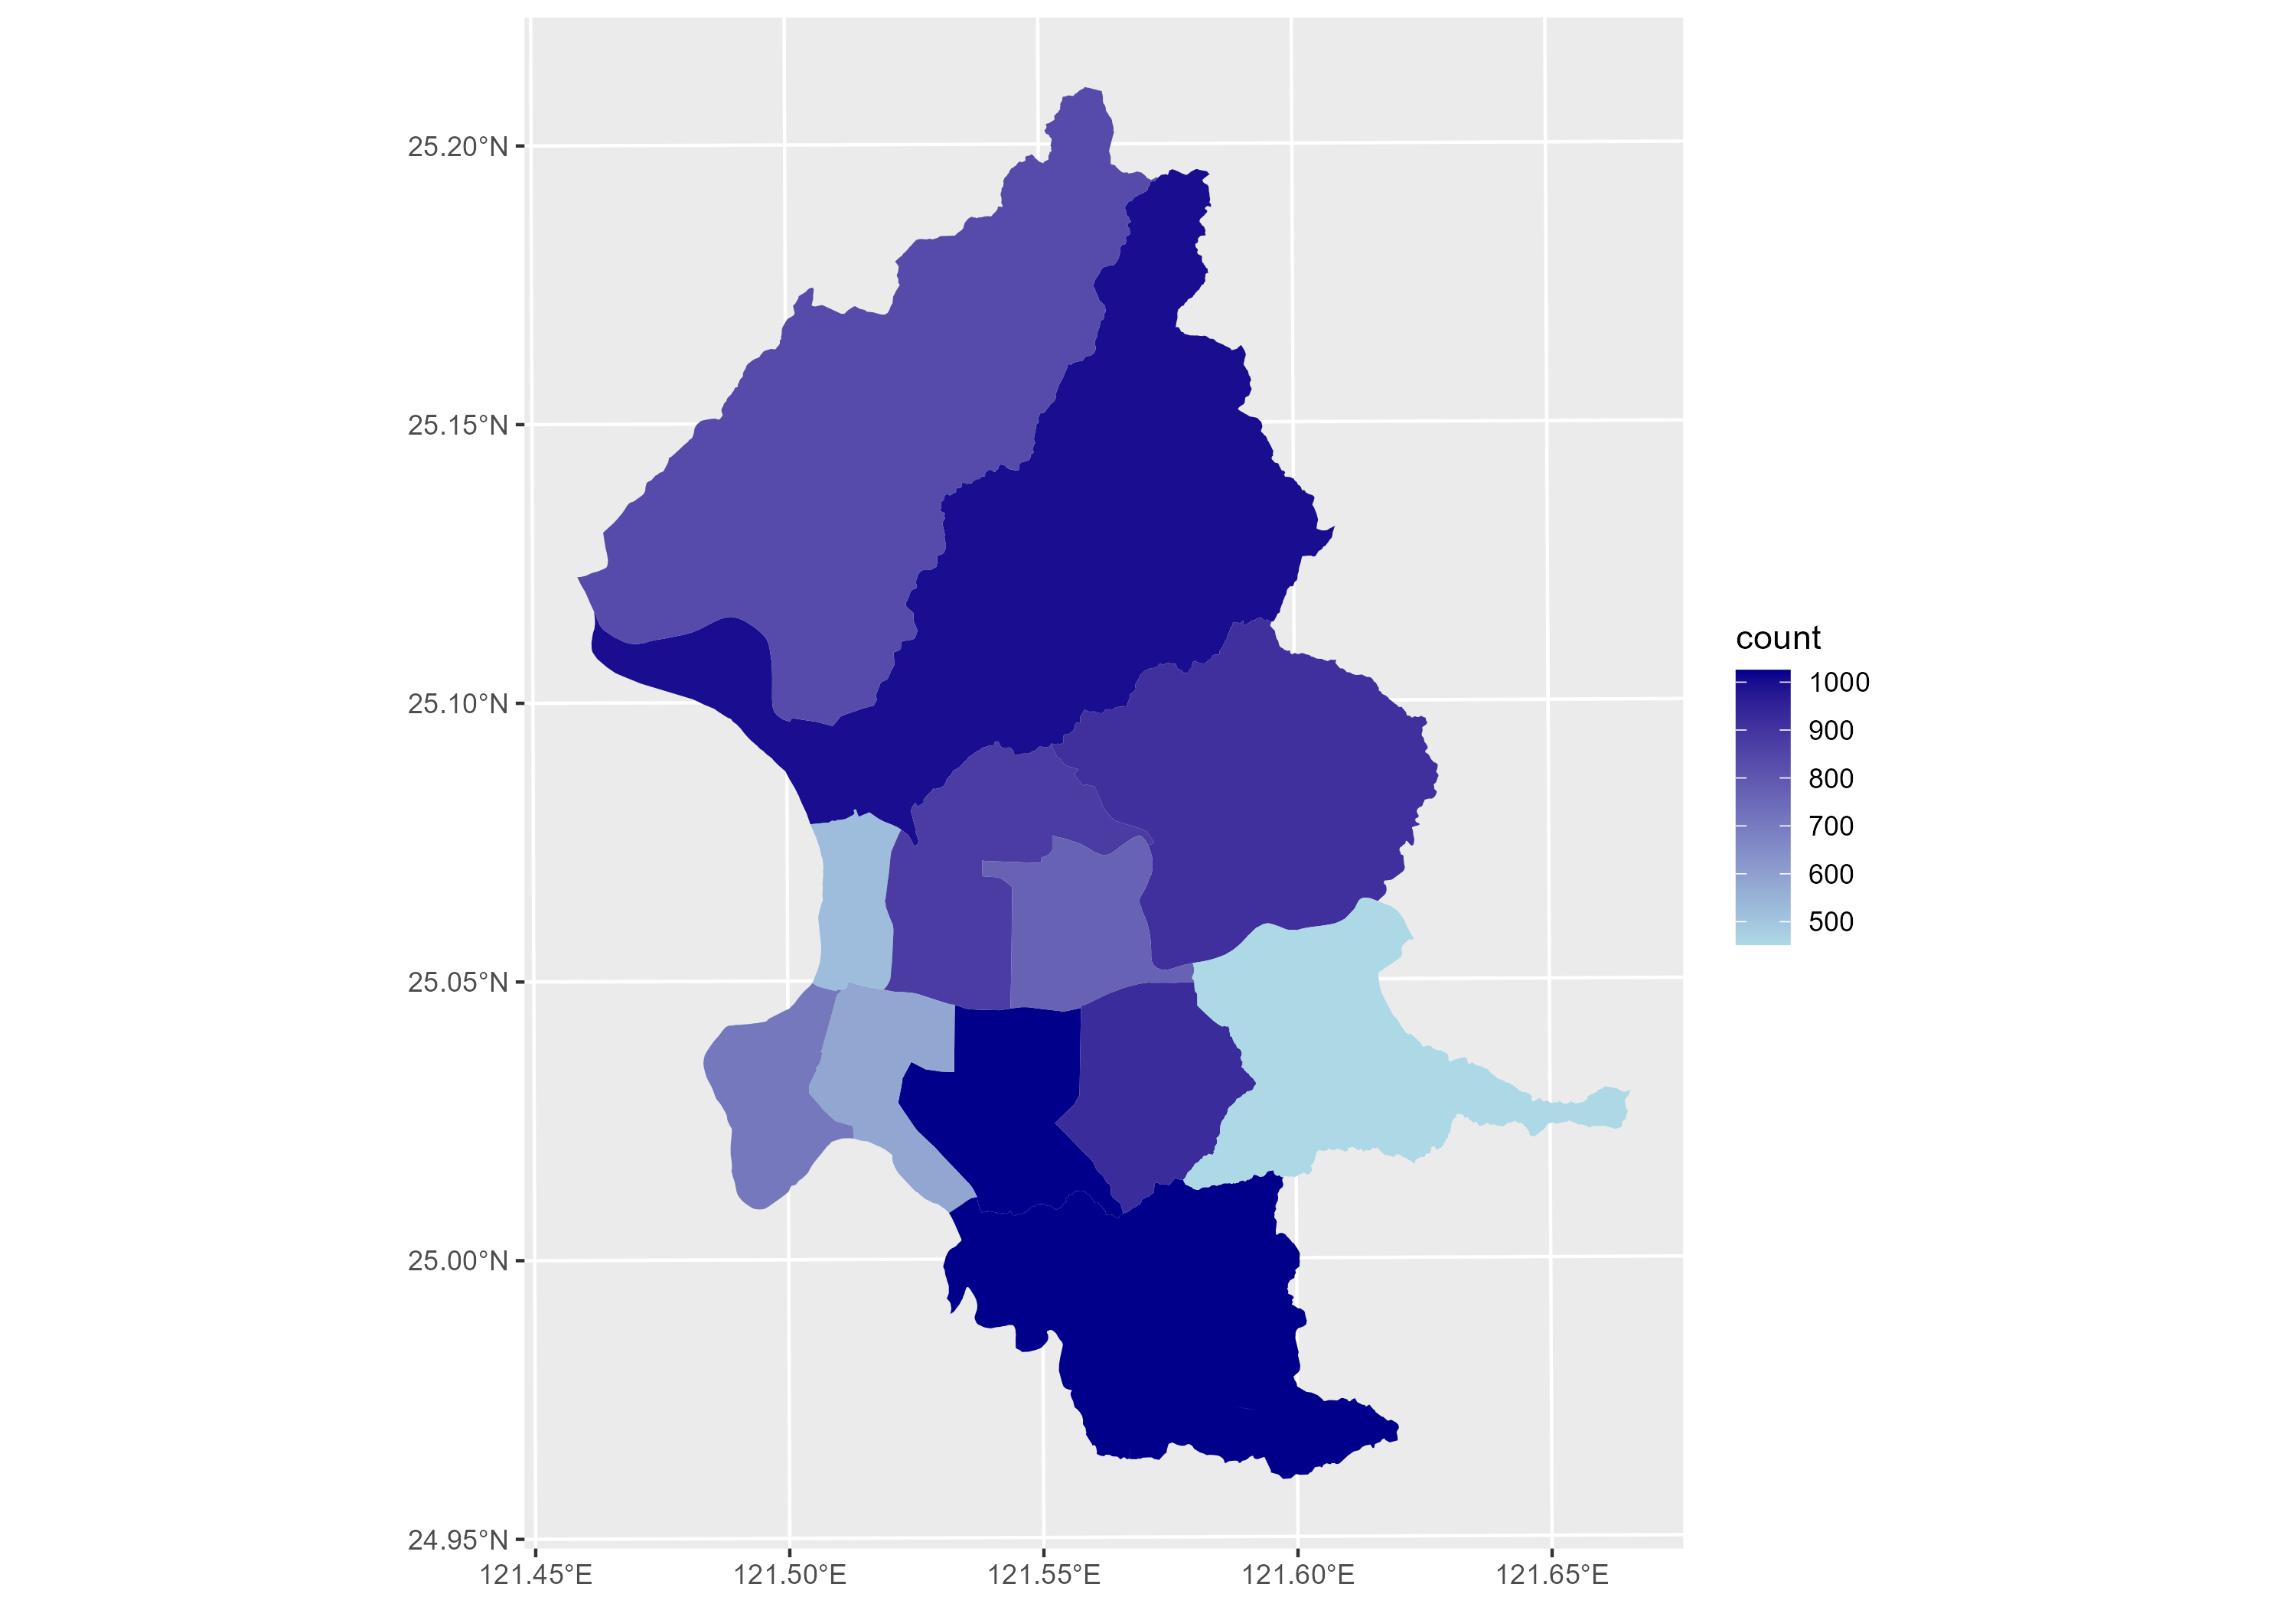
\includegraphics[width=.7\textwidth]{figure/count.png}
		\end{figure}
	\end{center}
\end{frame}




\begin{frame}[fragile]{Spatial Aggregation}{R Code}
\begin{lstlisting}
lie_price <- group_by(house_join, LIE_CODE) %>%
summarise(mean_price = mean(h_price_m2))
\end{lstlisting}
\begin{itemize}
	\item This code performs spatial aggregation to calculate the mean price per square meter (`mean\_price`) for different locations identified by the `LIE\_CODE` variable (村里代碼).
	\vspace{0.2cm}
		\end{itemize}
\end{frame}




\begin{frame}[fragile]{Spatial Aggregation}{R Output}
	
	\tiny
	
\begin{lstlisting}
Simple feature collection with 6 features and 2 fields
Geometry type: MULTIPOINT
Dimension:     XY
Bounding box:  xmin: 306087 ymin: 2771630 xmax: 307580 ymax: 2773221
Projected CRS: TWD97 / TM2 zone 121
# A tibble: 6 $\times$ 3
LIE_CODE   mean_price                               geometry
<chr>           <dbl>                       <MULTIPOINT [m]>
1 6300100002    171924. ((306971 2773055), (306978 2773026), \ldots{}
2 6300100003    246851. ((306087 2772446), (306129 2772370), \ldots{}
3 6300100004    209986. ((306657 2772613), (306664 2772667), \ldots{}
\end{lstlisting}
	
\end{frame}




	
\begin{frame}[fragile]{Spatial Aggregation}{R Code}
\begin{lstlisting}
lie_price <- st_drop_geometry(lie_price)
\end{lstlisting}
\begin{itemize}
	\item This code removes the geometry column from the `lie\_price` data frame.
	\vspace{0.2cm}
	\begin{itemize}
		\item The `\textbf{st\_drop\_geometry()}` function is used to drop the spatial geometry column, leaving only the non-spatial attributes in the data frame.
	\end{itemize}
\end{itemize}

\begin{lstlisting}
lie_price <- left_join(town, lie_price) %>% na.omit()
\end{lstlisting}
\begin{itemize}
	\item This code performs a left join operation between the `town` spatial data frame and the modified `lie\_price` data frame.
	\vspace{0.2cm}
	\begin{itemize}
		\item The `\textbf{left\_join()}` function joins the two data frames based on a common key, which is an identifier related to locations.
		\item `\textbf{na.omit()}` function to remove rows with missing values, if any exist in the result.
	\end{itemize}
\end{itemize}
\end{frame}


\begin{frame}{Spatial Aggregation}{Housing Price by 里}{}
	\begin{center}
		\begin{figure}[p]
			\centering
			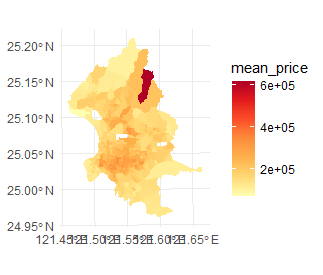
\includegraphics[width=.9\textwidth]{figure/h_price_lie.png}
		\end{figure}
	\end{center}
\end{frame}

\begin{frame}[fragile]{Spatial Aggregation}{R Output}
	
	\tiny
	
\begin{lstlisting}
# A tibble: 6 $\times$ 2
LIE_CODE   mean_price
<chr>           <dbl>
1 6300100002    171924.
2 6300100003    246851.
3 6300100004    209986.
\end{lstlisting}

	
\end{frame}








\begin{frame}{Spatial Buffering}{Overview}

	
	\begin{itemize}
		\item A buffer in spatial analysis refers to a zone around a specific spatial object, measured in units of distance or time
					\vspace{0.2cm}
			\begin{itemize}
			\item \textbf{Proximity Analysis:} Identifying geographic features within a specific distance.
			\vspace{0.2cm}
			\item \textbf{Impact Estimation:} Assessing potential areas affected by certain events or developments.
			
		\end{itemize}
		
	\end{itemize}
\end{frame}





\begin{frame}[fragile]{Spatial Buffering}{R Code}
\begin{lstlisting}
mrt_station_buffer <- st_buffer(mrt_station_taipei, 250)
\end{lstlisting}
\begin{itemize}
\item The `\textbf{st\_buffer()}` function creates a buffer around the points in the  `mrt\_station\_taipei` data frame.
	\vspace{0.2cm}
	\begin{itemize}
		\item The buffer size is specified as `250`, which likely represents a distance in the coordinate system's units (e.g., meters).
	\end{itemize}
\end{itemize}
\end{frame}




\begin{frame}{Spatial Interpolation}{Overview}
	
	
	\begin{itemize}
		\item Spatial interpolation is an analytical technique used in geographic studies to:
		\vspace{0.2cm}
		\item Estimate unknown values at geographical locations where measurements are unavailable
					\vspace{0.2cm}
		\begin{itemize}
			\item Filling gaps in geographical data utilizing known data from surrounding points
			\vspace{0.2cm}
			\item Create continuous data representations across a landscape
			
		\end{itemize}

	\end{itemize}
\end{frame}


\begin{frame}{Spatial Interpolation}{Overview}
	\begin{center}
		\begin{figure}[p]
			\centering
			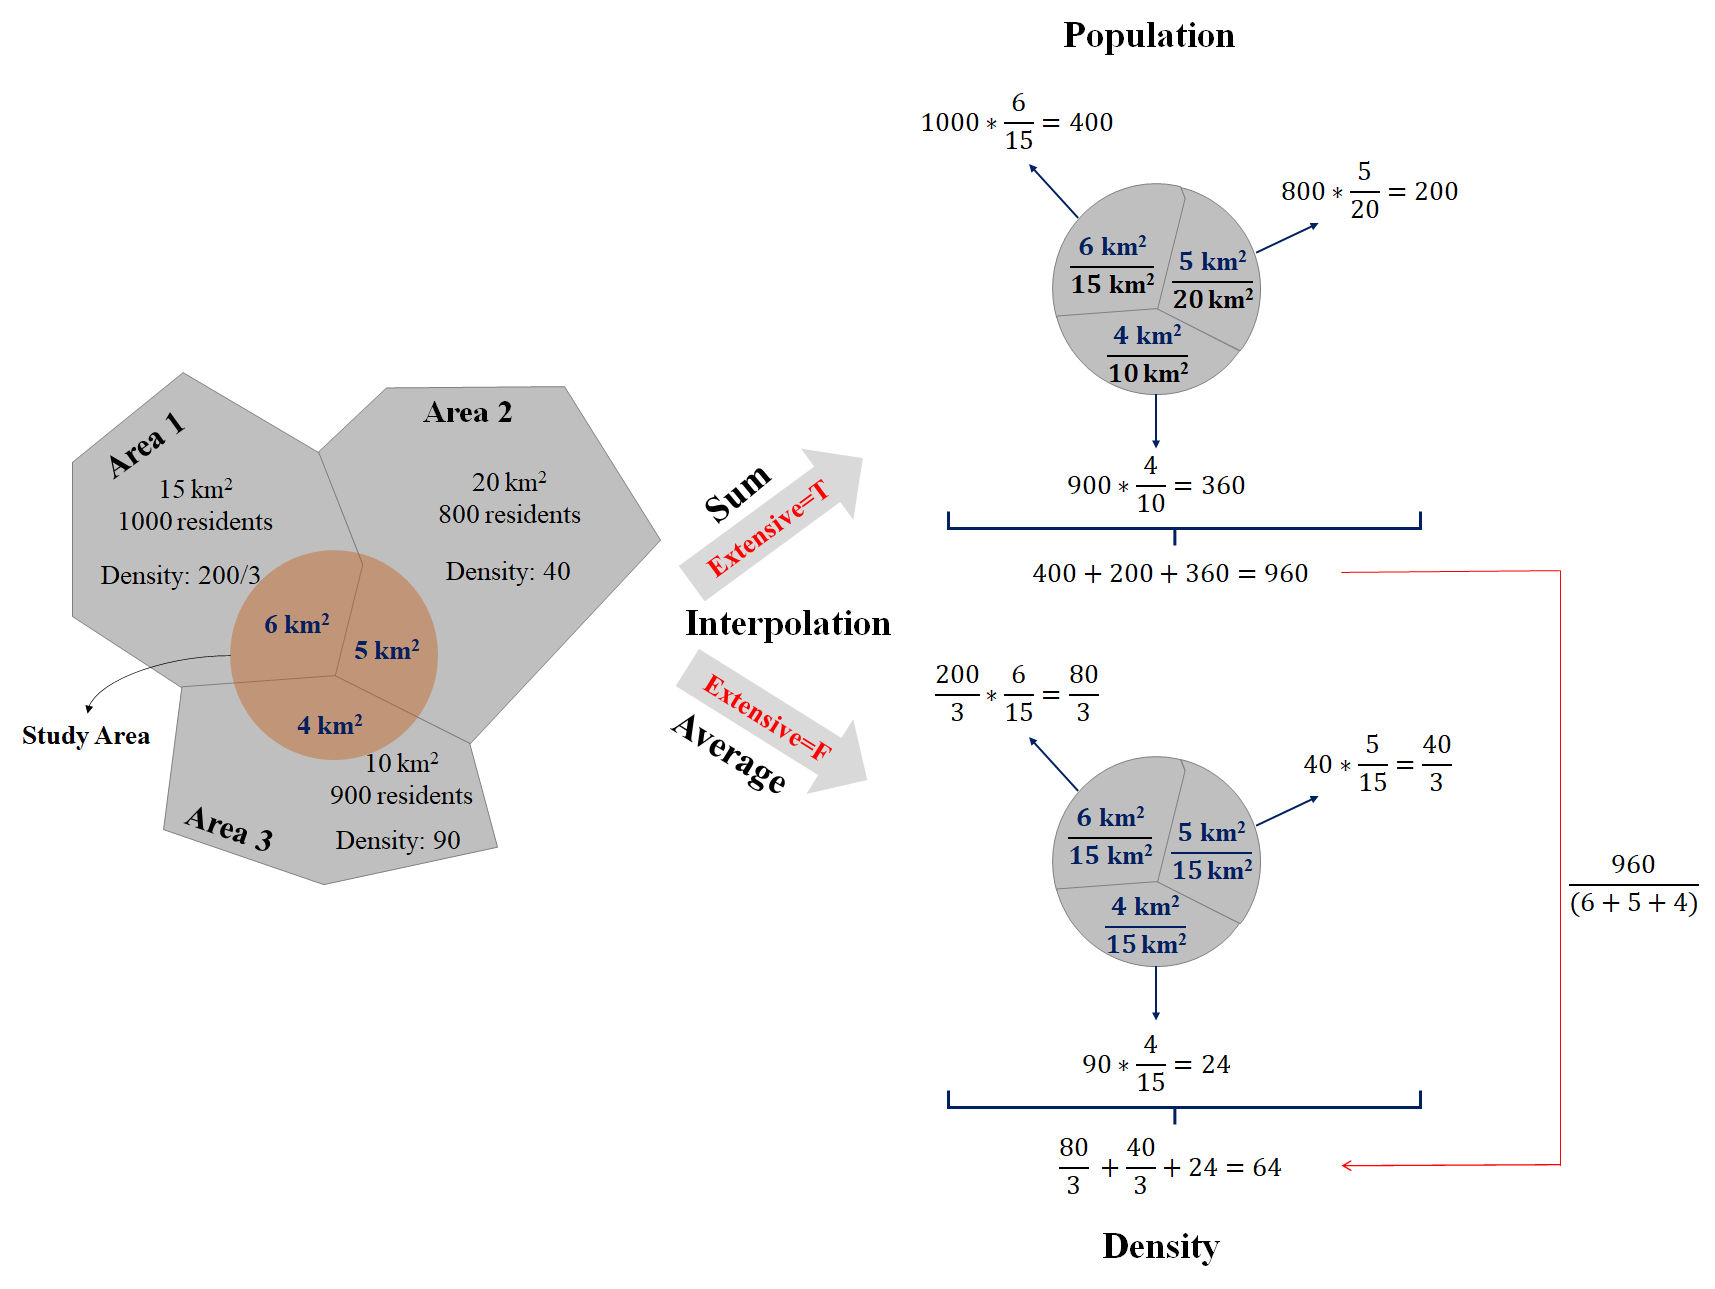
\includegraphics[width=.9\textwidth]{figure/interpolation.png}
		\end{figure}
	\end{center}
\end{frame}




\begin{frame}[fragile]{Spatial Interpolation}{R Code}
\begin{lstlisting}
mrt_interpo <- st_interpolate_aw(lie_price["mean_price"],
mrt_station_buffer,
extensive = TRUE)
\end{lstlisting}

\begin{itemize}
	\item The \textbf{st_interpolate_aw()}` function performs spatial interpolation to estimate values of the `mean\_price` variable from the `lie\_price` data frame at the locations represented by the buffered `mrt\_station\_buffer`.
	\vspace{0.2cm}
	
\end{itemize}
\end{frame}



\begin{frame}[fragile]{Spatial Interpolation}{R Output}
\begin{center}
	\begin{figure}[p]
		\centering
		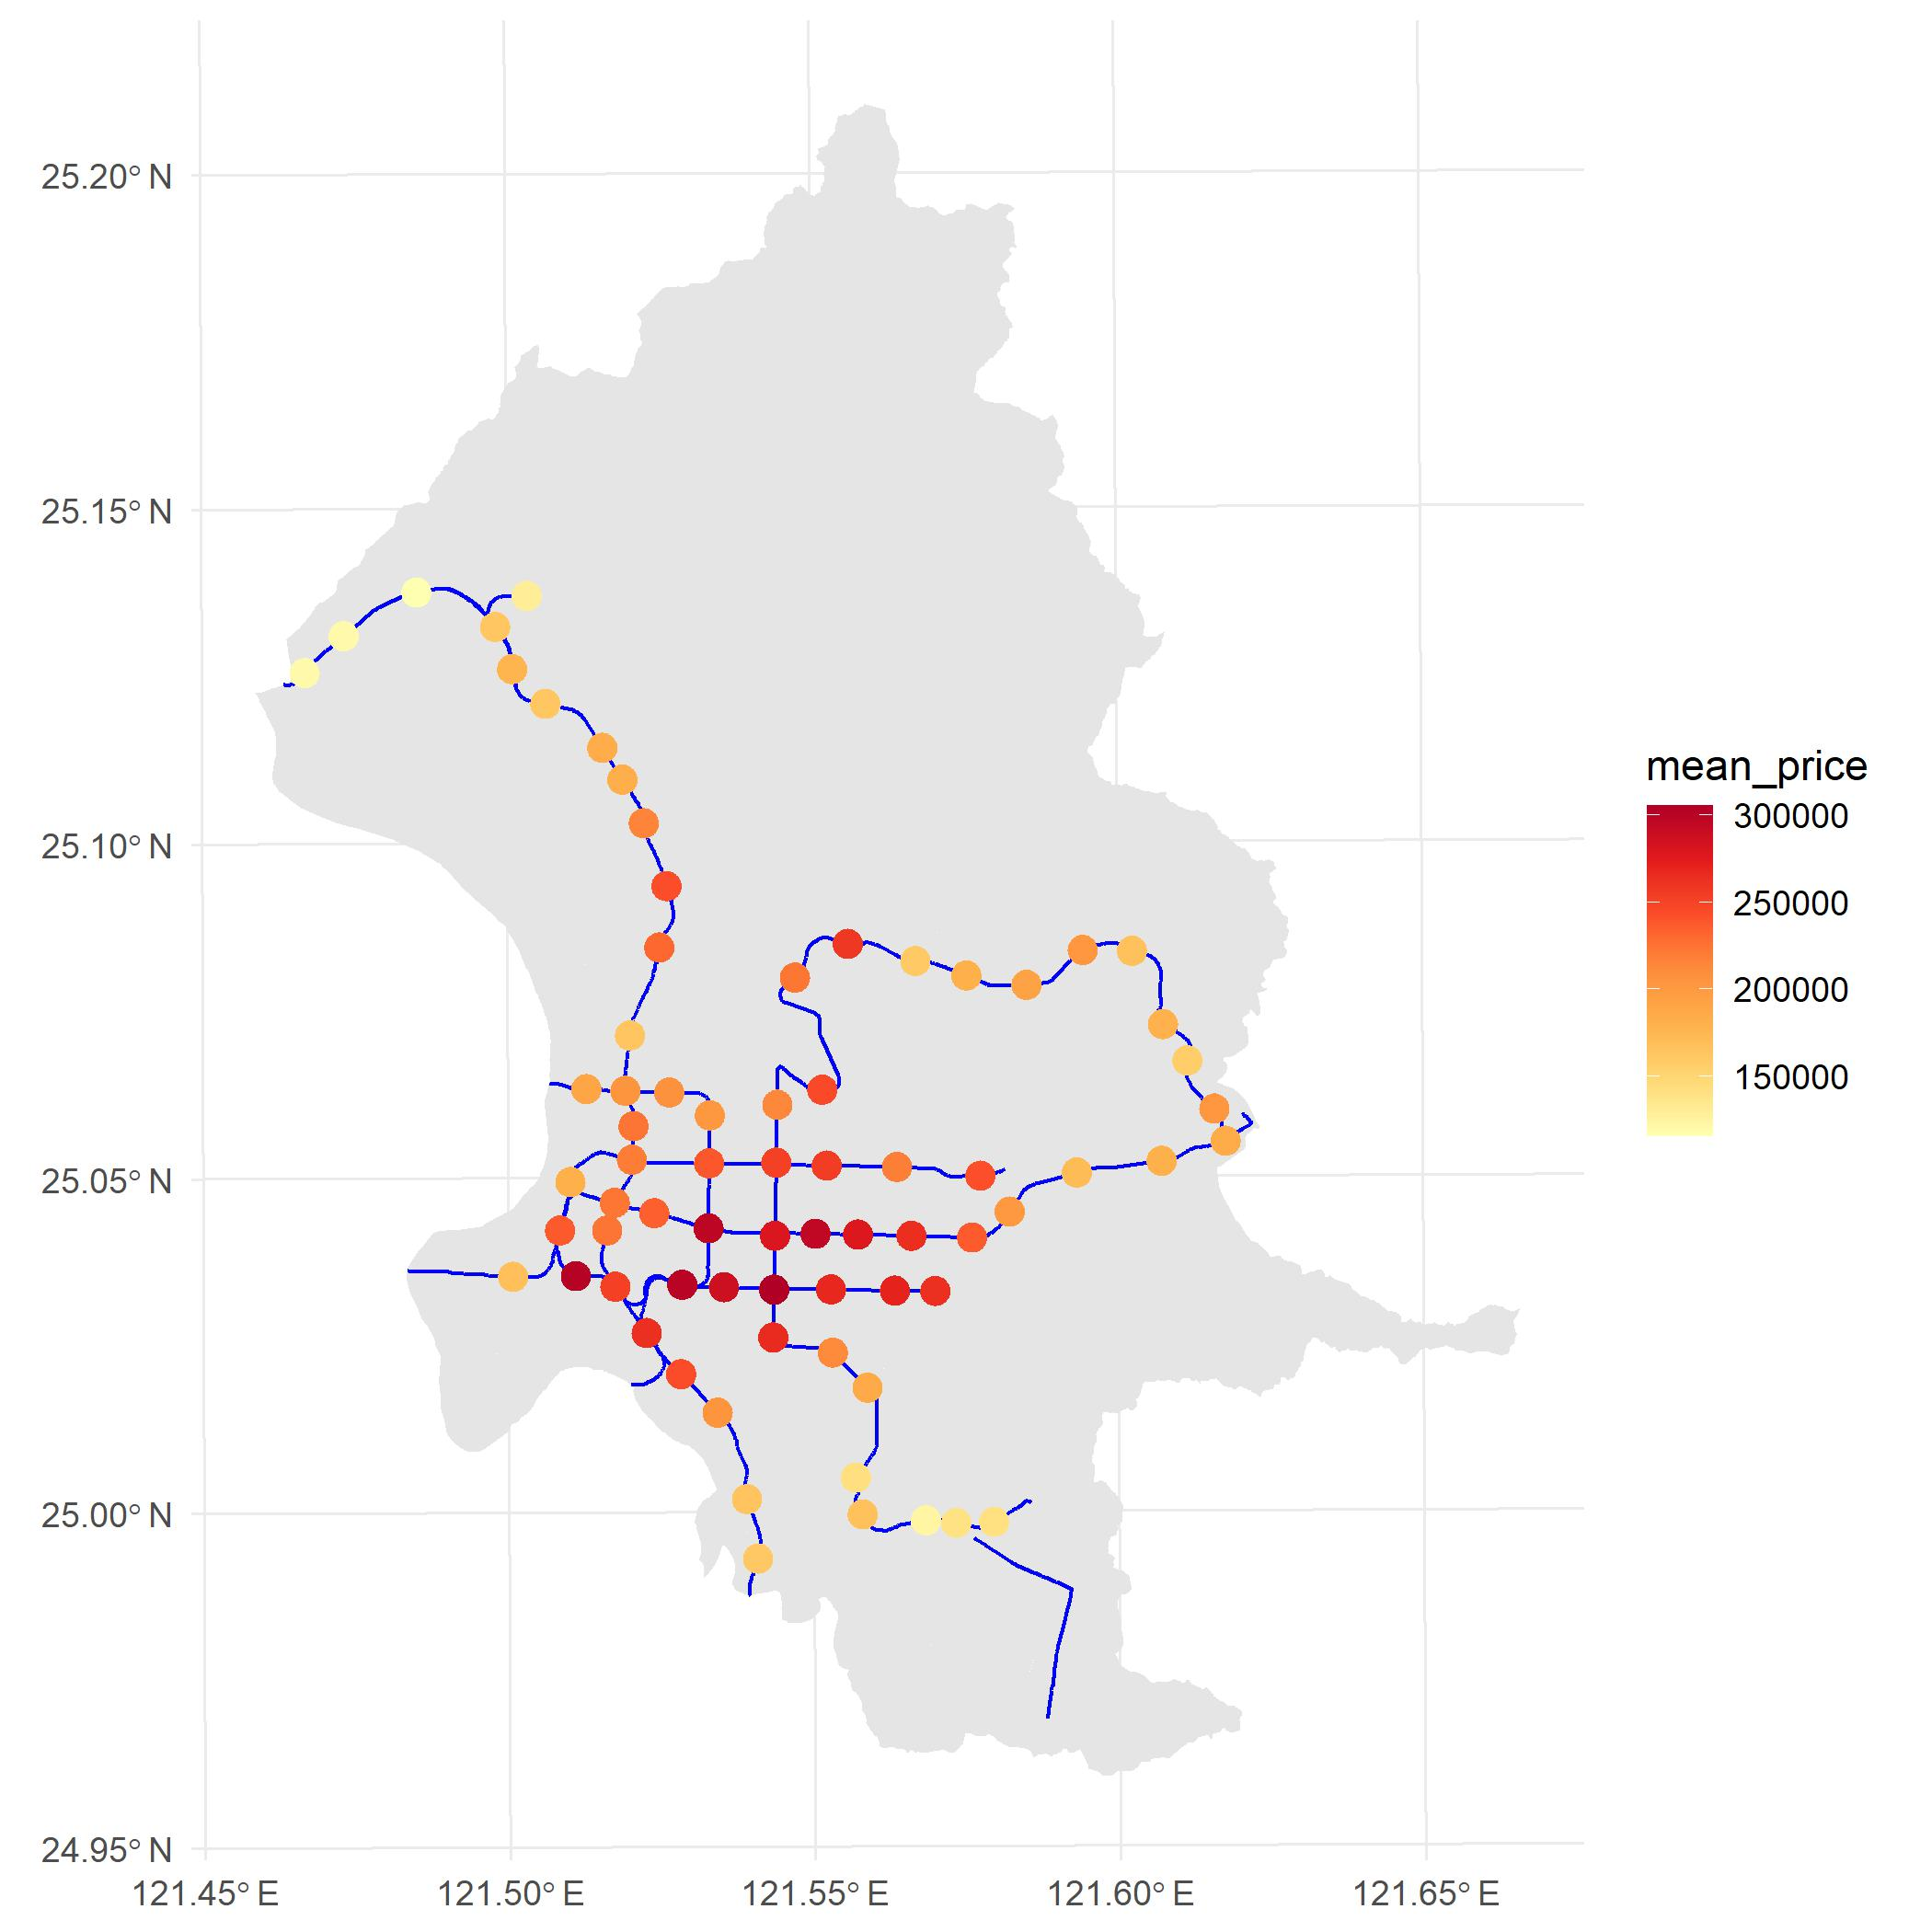
\includegraphics[width=.7\textwidth]{figure/mrt_interpo_plot.jpg}
	\end{figure}
\end{center}
\end{frame}





\begin{frame}[fragile]{Spatial Measurement -- Area}{R Code}
\begin{lstlisting}
dist_area <- st_area(district)
\end{lstlisting}

\begin{itemize}
	\item The `\textbf{st\_area()}` function calculates the areas of the districts
	\vspace{0.2cm}
	\begin{itemize}
		\item It computes the area of each polygon in the `district` data frame
	\end{itemize}
\end{itemize}
\end{frame}



\begin{frame}[fragile]{Spatial Measurement -- Area}{R Output}

\tiny

\begin{lstlisting}
Units: [m^2]
[1] 13918274  7540905 11242231 31943143 57381712 21953874
[7] 61078059  4768692 11341341 31249341  8681328  7450219
\end{lstlisting}


\end{frame}


\begin{frame}[fragile]{Spatial Measurement -- Length}{R Code}
\begin{lstlisting}
mrt_length <- st_length(mrt_line)
\end{lstlisting}

\begin{itemize}
	\item The \textbf{st\_length()} function calculates the lengths of the MRT stations.
	\vspace{0.2cm}
\end{itemize}
\end{frame}




\begin{frame}[fragile]{Spatial Measurement -- Length}{R Output}

\tiny

\begin{lstlisting}
Units: [m]
[1] 2473.6302 1071.9619 2219.4709 1070.2943 1133.0579
[6]  916.3198
\end{lstlisting}


\end{frame}






\begin{frame}[fragile]{Spatial Measurement -- Perimeter}{R Code}
\begin{lstlisting}
dist_border <- st_boundary(district)
\end{lstlisting}

\begin{itemize}
	\item The `\textbf{st\_boundary()}` function gets boundaries of the districts
	\vspace{0.2cm}

\end{itemize}

\begin{lstlisting}
dist_peri <- st_length(dist_border) 
\end{lstlisting}

\begin{itemize}
	\item The `\textbf{st\_length()}` function calculates the lengths of the district boundaries.
	\vspace{0.2cm}
\end{itemize}


\end{frame}


\begin{frame}[fragile]{Spatial Measurement -- Perimeter}{R Output}

\tiny

\begin{lstlisting}
Units: [m]
[1] 32180.99 16395.05 30570.30 36769.93 49349.66 37274.69
[7] 85812.19 19243.09 23529.49 40296.29 20646.82 13711.05
\end{lstlisting}


\end{frame}





\begin{frame}{Spatial Measurement -- Distance}{Overview}


\begin{itemize}
	\item To find the shortest distance between two geometries.
\begin{center}
	\begin{figure}[p]
		\centering
		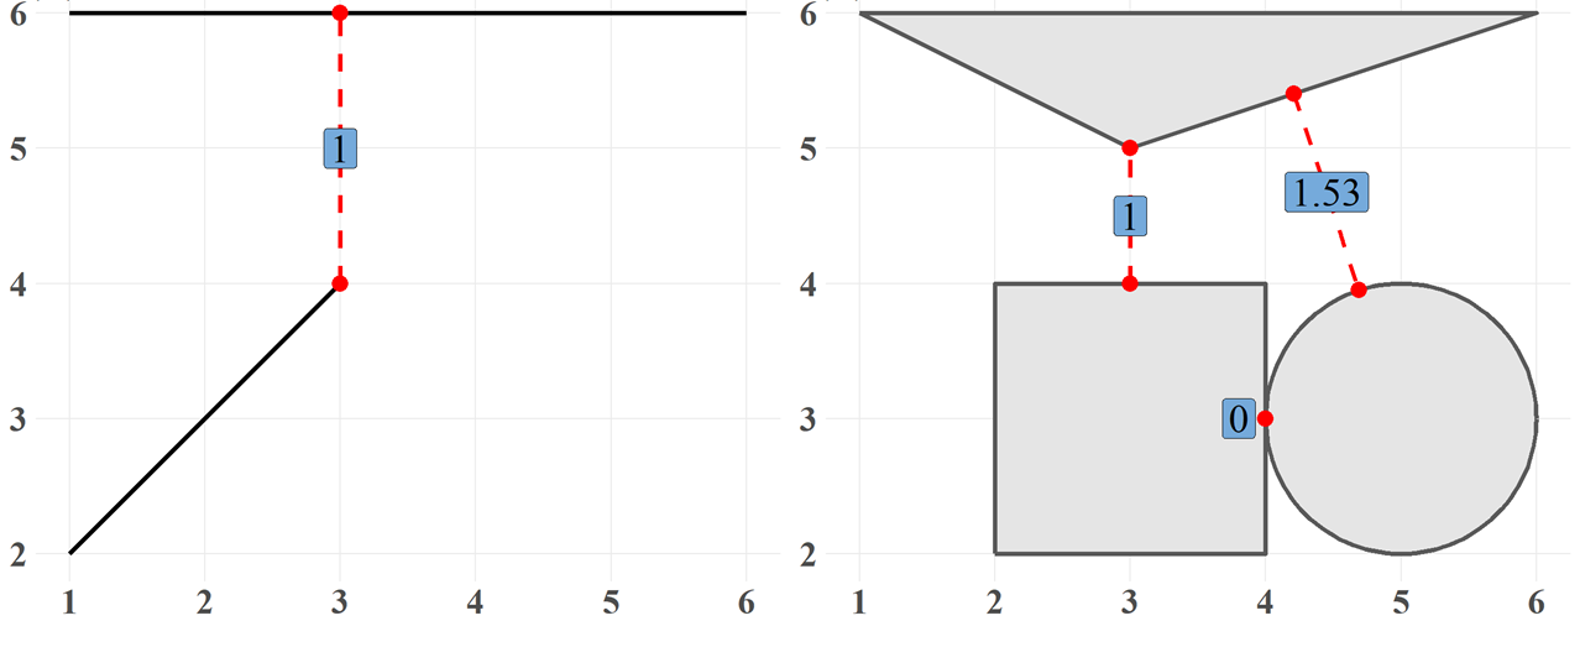
\includegraphics[width=.9\textwidth]{figure/distance.png}
	\end{figure}
\end{center}
	
\end{itemize}
\end{frame}


\begin{frame}{Spatial Measurement -- Distance}{R Code}


\small

\begin{itemize}
	\item \textbf{st\_distance(data1):} $M_{n \times n}$
	- the distance between each geometry element within the geographic data
			\vspace{0.2cm}
	\item \textbf{st\_distance(data1, data2):} $M_{n \times k}$
	- the distance between each paired geometry element from two geographic datasets.
			\vspace{0.2cm}
	\item \textbf{st\_distance(data1, data2, by\_element=T):} $M_{1 \times n}(M_{1 \times k})$
	- the distance between each pairwise matched geometry element from two geographic datasets.- $n = k$
			\vspace{0.2cm}
	\item \textbf{st\_nearest\_feature(object\_data, nearest\_feature)}
\end{itemize}
\end{frame}


\begin{frame}[fragile]{Spatial Measurement -- Distance}{R Code}
\begin{lstlisting}
near_mrt <- st_nearest_feature(house, mrt_station)
\end{lstlisting}

\begin{itemize}
	\item The `\textbf{st\_nearest\_feature()}` function calculates the nearest metro (MRT) station to each house location in the `house` data frame.
	\vspace{0.2cm}
	\begin{itemize}
		\item It calculates the nearest feature (in this case, MRT station) for each house and returns an index indicating the nearest station.
	\end{itemize}
\end{itemize}
\end{frame}




\begin{frame}[fragile]{Spatial Measurement -- Distance}{R Code}
\begin{lstlisting}
house$near_mrt <- mrt_station$MARKNAME1[near_mrt]

house$dis_mrt <- st_distance(house,
mrt_station[near_mrt,],
by_element = TRUE)
\end{lstlisting}

\begin{itemize}
		\item \textbf{st\_distance()} calculates the distance between each house and its nearest MRT station.
	\vspace{0.2cm}
	\begin{itemize}
		\item The `\textbf{by\_element = TRUE}` argument indicates that distances should be computed for each element separately.
		\vspace{0.2cm}
		
	\end{itemize}
\end{itemize}
\end{frame}




\begin{frame}[fragile]{Spatial Measurement -- Distance}{R Output}

\tiny

\begin{lstlisting}
## Simple feature collection with 6 features and 3 fields
## Geometry type: POINT
## Dimension: XY
## Bounding box: xmin: 301535 ymin: 2764405 xmax: 312256 ymax: 2781542
## Projected CRS: TWD97 / TM2 zone 121
## address near_mrt
## 1 台北市南港區興南街150號10樓 臺北捷運昆陽站_BL21
## 2 臺北市信義區安康里29鄰松勇路69巷10號17樓 臺北捷運象山站_R02
## 3 臺北市內湖區康寧路三段187號七樓 臺北捷運東湖站_BR22
## dis_mrt geometry
## 1 727.47014 [m] POINT (310403 2771990)
## 2 38.06205 [m] POINT (307543 2769572)
## 3 325.02846 [m] POINT (311748 2773676)
\end{lstlisting}


\end{frame}









\title[]  
{Empirical Example in Economics}


\author 
{}

%\institute{Institute of Economics, Academia Sinica  \\ Econ, NTU}
%\institute{Institute of Economics, Academia Sinica  \\ IMES/IDAS, NCCU}
\institute{}

%\author 
%{楊子霆 \\ 中研院經濟所}

%\institute 
%{中正大學國際經濟專題研討}




\date
{}


\begin{frame}{}
\titlepage
\end{frame}



\begin{frame}{Empirical Example: Nathan Nunn (2008)}
% ... (Slide 2 content, as provided earlier) ...

Nathan Nunn (2008), ``\textbf{The Long-term Effects of Africa's Slave Trades}", QJE
					\vspace{0.2cm}
\begin{itemize}
	\item Does the intensity of slave trade affect economic development of African countries centuries later?
\end{itemize}
\end{frame}



	


\begin{frame}{Background}
% ... (Slide 2 content, as provided earlier) ...
\begin{itemize}
	\item \textbf{Manning (1990, p. 124):} "Slavery was corruption: it involved theft, bribery, and exercise of brute force as well as ruses."
					\vspace{0.2cm}
					\begin{itemize}
	\item "Slavery thus may be seen as one source of precolonial origins
	for modern corruption."
\end{itemize}
\end{itemize}
\end{frame}


\begin{frame}{Background}
\begin{itemize}
	\item Between 1400 and 1900, Africa experienced four simultaneous slave trades
						\vspace{0.2cm}
									\begin{itemize}		
	\item Total volume of slaves traded unprecedented: $\sim$18 million
						\vspace{0.2cm}
	\item Slaves taken through warfare, raiding, kidnapping within Africa
						\vspace{0.2cm}
	\end{itemize}				
	\item Adverse effects: social/ethnic fragmentation, political instability, weakened states
\end{itemize}
\end{frame}


\begin{frame}{Data}

\begin{itemize}
\item \textbf{Raw data:}
							\vspace{0.2cm}
\begin{itemize}
	\item Number of slaves shipped from each African country in each century between 1400 and 1900
							\vspace{0.2cm}
	\item Shipping records of trans-Atlantic slave trade in each African country 
							\vspace{0.2cm}
	\item Historical documents on ethnic identities of exported slaves
\end{itemize}
\end{itemize}
\end{frame}



\begin{frame}{Data}{Combining Shipping and Ethnicity Data}
\begin{itemize}
	\item \textbf{Objective:} Accurately estimate the number of slaves shipped from each African country.
								\vspace{0.2cm}
	\item \textbf{Challenge:} Coastal shipping data doesn't account for inland origins (e.g., slaves from Country B shipped from Country A's ports).
	\begin{itemize}
									\vspace{0.2cm}
		\item Slaves from Country B shipped from Country A's ports
	
	\end{itemize}
\end{itemize}
\end{frame}




\begin{frame}{Data}{Combining Shipping and Ethnicity Data}
\begin{itemize}
	\item \textbf{Approach:}
	\begin{itemize}
										\vspace{0.2cm}
		\item Use shipping data to calculate initial figures from coastal countries.
										\vspace{0.2cm}
		\item Apply ethnicity ratios to adjust figures for landlocked countries.
												\vspace{0.2cm}
	\end{itemize}


\item \textbf{Example:} 
								\vspace{0.2cm}
	\begin{itemize}
\item 100,000 slaves shipped from Country A
								\vspace{0.2cm}
			\begin{itemize}						
			\item Ratios: Country A to B is 4:1.
									\vspace{0.2cm}
		\item Estimates: 80,000 from Country A, 20,000 each from Countries B.										\vspace{0.2cm}
								\end{itemize}
								
\item 250,000 slaves shipped from Country C.
										\vspace{0.2cm}
					\begin{itemize}						
\item Ratios: Country C to D to E is 3:1:1.
										\vspace{0.2cm}
\item Estimates: 150,000 from Country C, 50,000 each from Countries D and E.
\end{itemize}
\end{itemize}
\end{itemize}
\end{frame}



\begin{frame}{Data}{Combining Shipping and Ethnicity Data}



	\begin{center}
		\begin{figure}[p]
			\centering
			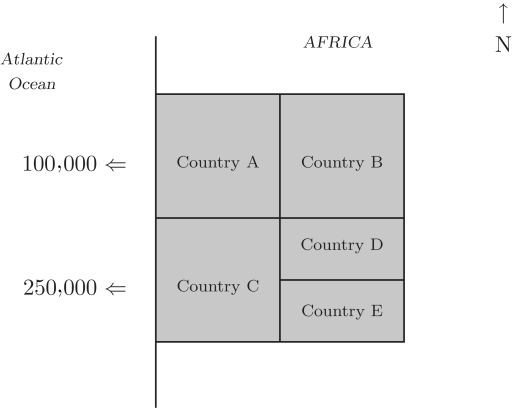
\includegraphics[width=.9\textwidth]{figure/slave_f1.png}
		\end{figure}
	\end{center}
	

\end{frame}



\begin{frame}{Graphical Evidence}

	\begin{itemize}
\item A robust negative relationship exists between slave exports and income.

	\end{itemize}	


\begin{figure}
	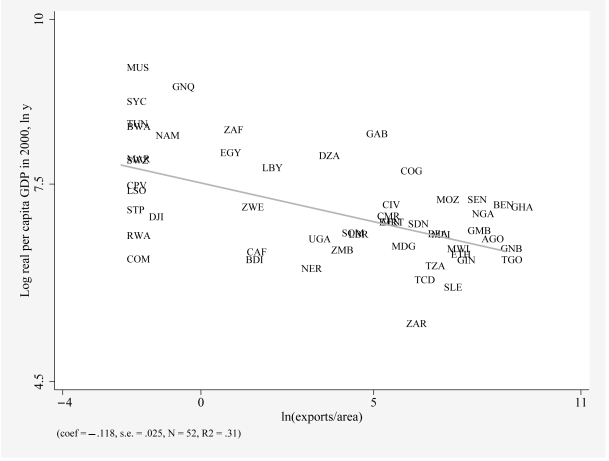
\includegraphics[width=0.8\textwidth]{figure/slave_f2.png}
\end{figure}

\end{frame}



\begin{frame}{Empirical Specification}{OLS Estimation}

\begin{equation*}
\ln y_i = \beta_0 + \beta_1 \ln(\text{exports}_i/\text{area}_i) + \mathbf{C}_i\delta + \mathbf{X}_i\gamma + \epsilon_i
\end{equation*}

	\begin{itemize}
	\item $\ln y_i$: log of real per capita GDP in country
	$i$ in 2000
											\vspace{0.2cm}
	\item $\ln(\text{exports}_i/\text{area}_i)$: log of the total
	number of slaves exported between 1400 and 1900 normalized by
	land area
												\vspace{0.2cm}
	 \item $\mathbf{C}_i$: a vector of dummy variables that
	indicate the origin of the colonizer prior to independence
												\vspace{0.2cm}
	 \item $\mathbf{X}_i$: a vector of control variables that are meant
	 to capture differences in countries' geography and climate
	
\end{itemize}

\end{frame}



\begin{frame}{Results}{OLS Estimates}

\begin{figure}
	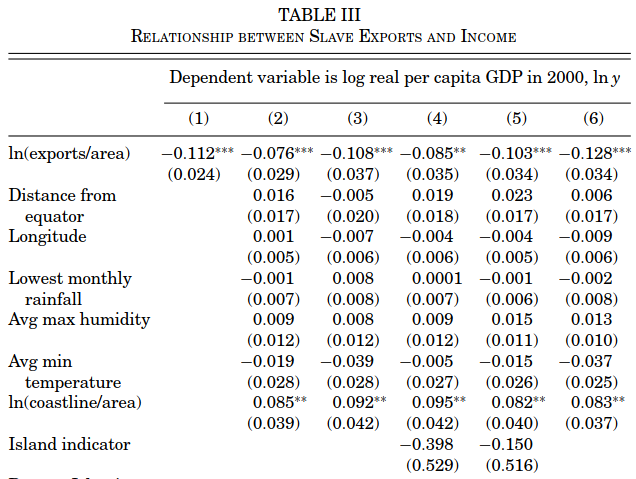
\includegraphics[width=0.8\textwidth]{figure/slave_t3.png}
\end{figure}

\end{frame}



\begin{frame}{Selection versus Causation}
	\begin{itemize}
\item Two competing hypotheses:
												\vspace{0.2cm}
\begin{enumerate}
\item \textbf{Causation:} Slave trades had a causal negative impact on economic development
												\vspace{0.2cm}
\item \textbf{Selection:} Underdeveloped areas selected into slave trades
\end{enumerate}
												\vspace{0.2cm}
\item Need to distinguish between the two stories.

\end{itemize}
\end{frame}

\begin{frame}{Historic Evidence on Selection}

\begin{itemize}
\item Initially, Europeans sought prosperous trade partners
												\vspace{0.2cm}
		\begin{itemize}										
\item Coastal raiders targeted densely populated interior states
												\vspace{0.2cm}
\item Population density in 1400 positively correlated with slave exports
\end{itemize}

												\vspace{0.2cm}
%\item Evidence contradicts underdevelopment selection hypothesis.

\end{itemize}
\end{frame}



\begin{frame}{Historic Evidence on Selection}

\begin{figure}
	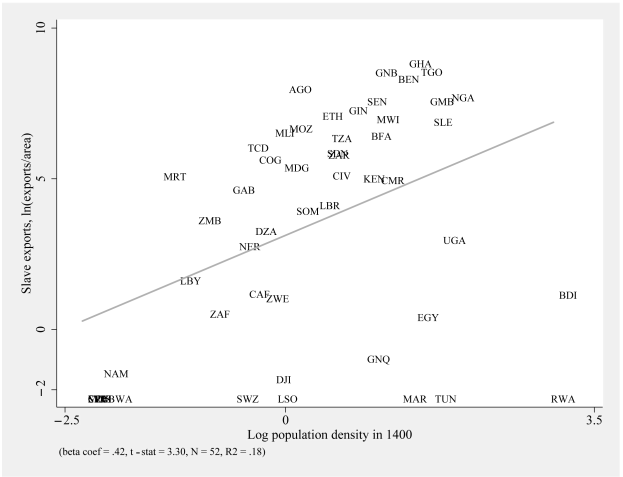
\includegraphics[width=0.8\textwidth]{figure/slave_f3.png}
\end{figure}

\end{frame}




\begin{frame}{Causal Estimation}{Instrumental Variable for Slave Trade}

\begin{itemize}

	\vspace{0.2cm}
	\item IV for slave trade: 
	\begin{itemize}
		\vspace{0.2cm}
		\item Distance to the nearest slave trade center in the Americas
				\vspace{0.2cm}
			\begin{itemize}
		\item Sailing distance from the point on the coast closest to the country's centroid to the nearest trade hub
			\end{itemize}
	\end{itemize}
\end{itemize}
\end{frame}

\begin{frame}{Causal Estimation}{Instrumental Variable for Slave Trade}
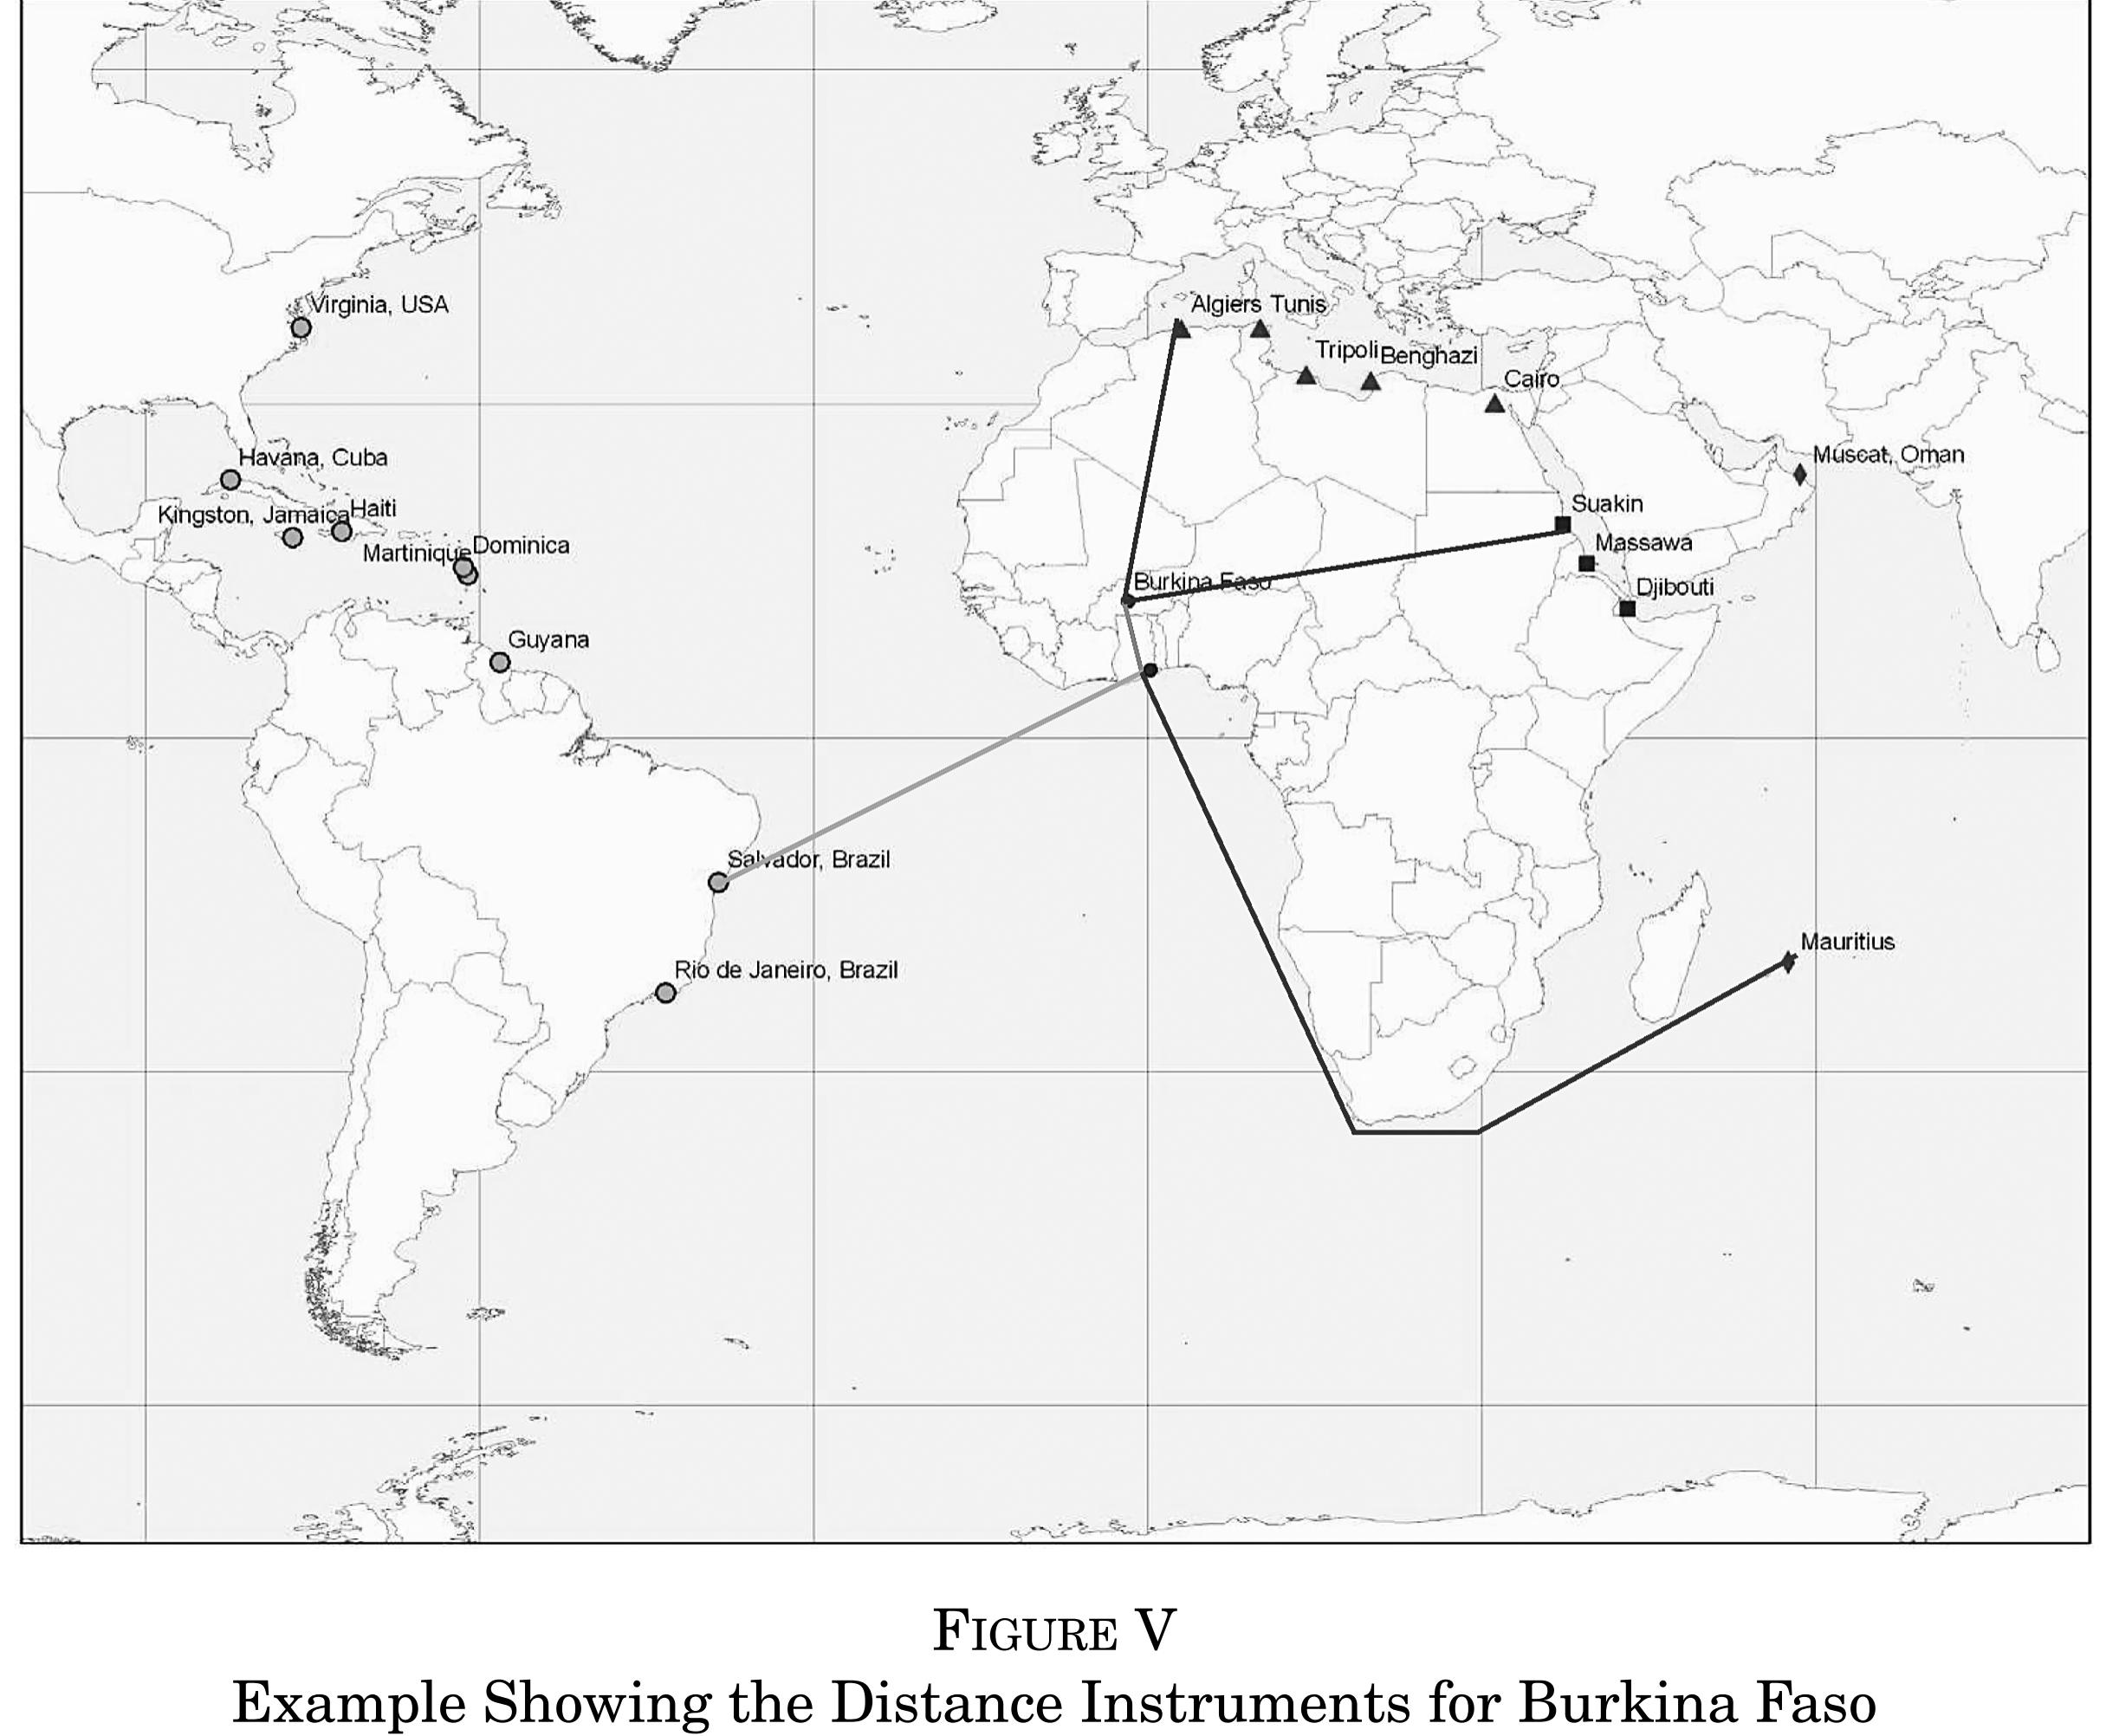
\includegraphics[width=.90\textwidth]{figure/slave_f5.jpg}

\end{frame}



\begin{frame}{Causal Estimation}{Instrumental Variable for Slave Trade}
\begin{itemize}
	
\item Identifying assumptions:
\begin{itemize}
	\item The location of trade hubs affect the location from which the slaves are taken but not vice versa
	\vspace{0.2cm}
	\item Distance only affects economic development through slave trade
\end{itemize}	
	\vspace{0.2cm}
\item Location of slave trade centers:
\begin{itemize}
\vspace{0.2cm}
\item Determined by climate suitability of plantation crops/location of mines
\vspace{0.2cm}
\item Not affected by the distance to Africa
\vspace{0.2cm}
\item Distance to slave markets $\neq$ Distance to other economic opportunities
\vspace{0.2cm}
\end{itemize}

\end{itemize}
\end{frame}




\begin{frame}{IV Estimates}{First Stage}

\begin{figure}
	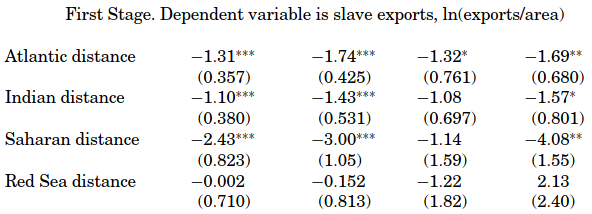
\includegraphics[width=0.8\textwidth]{figure/slave_t4.png}
\end{figure}

\end{frame}


\begin{frame}{IV Estimates}{Second Stage}

\begin{figure}
	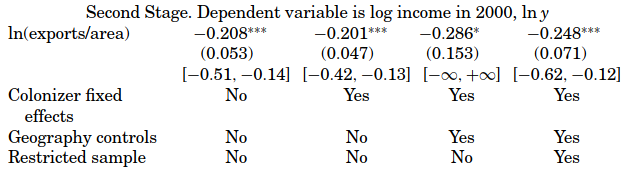
\includegraphics[width=0.8\textwidth]{figure/slave_t5.png}
\end{figure}

\end{frame}




\begin{frame}{Main Findings}

\begin{itemize}
	\item Robust negative relationship between slave exports and income
	\vspace{0.2cm}
	\item IV estimates confirm relationship likely causal

\end{itemize}

\end{frame}


\begin{frame}{Mechanism}

\begin{itemize}
\item Slave trades associated with:
	\vspace{0.2cm}
\begin{itemize}
\item Ethnic fractionalization and social fragmentation
	\vspace{0.2cm}
\item Political instability and weakened states

\end{itemize}
	\vspace{0.2cm}
\item Examine if data consistent with these channels.

\end{itemize}
\end{frame}



\begin{frame}{Conclusions}

\begin{itemize}
\item Suggests Africa's slave trades negatively impacted long-term development
	\vspace{0.2cm}
\item Findings complement evidence on New World slavery and institutions
	\vspace{0.2cm}
\item Illuminates channel via early state underdevelopment
\end{itemize}

\end{frame}




\begin{frame}{Implement Empirical Strategy using R}
		\begin{itemize}
		\item Implementing this IV requires:
			\vspace{0.2cm}
		\begin{itemize}
			\item Identifying the country's centroid
				\vspace{0.2cm}
			\item Determining the closest coastal point to the centroid
				\vspace{0.2cm}
			\item Calculating the distance to the nearest trade hub
		\end{itemize}
	\end{itemize}
	
\end{frame}


\begin{frame}{Implement Empirical Strategy using R}
\begin{itemize}
\item \textbf{Datasets:}
				\vspace{0.2cm}
\begin{itemize}
	\item Coast lines of the world
					\vspace{0.2cm}
	\item Country boundary in Africa
					\vspace{0.2cm}
	\item Boundary of ethnic regions in Africa
					\vspace{0.2cm}
	\item Trade hub locations
\end{itemize}
\end{itemize}
\end{frame}









\begin{frame}[fragile]{Load Spatial Data}{R Code}
\begin{lstlisting}
#--- coast line ---#
coast <-
sf::st_read(str_c(path, "10m_coastline.shp")) %>%
st_transform(3857)

#--- African countries ---#
countries <-
sf::st_read(str_c(path, "gadm36_africa.shp")) %>%
st_transform(3857)

#--- ethnic regions ---#
ethnic_regions <-
sf::st_read(str_c(path,"borders_tribes.shp")) %>%
st_transform(3857)
\end{lstlisting}

\begin{itemize}
	\item We first read all the GIS data we will be using in this demonstration and then reproject them to \textbf{epsg:3857}
	\vspace{0.2cm}
	
\end{itemize}
\end{frame}


\begin{frame}[fragile]{Load Spatial Data}{R Code}
\begin{lstlisting}
countries_simp <- rmapshaper::ms_simplify(countries)

g_countries <-
ggplot(data = countries_simp) +
geom_sf() +
theme_void()
\end{lstlisting}

\begin{itemize}
	\item We first simplify geometries of the African countries using \textbf{rmapshaper::ms\_simplify()}
	\vspace{0.2cm}
	
\end{itemize}
\end{frame}

\begin{frame}[fragile]{Load Spatial Data}{African Map}

\begin{figure}
	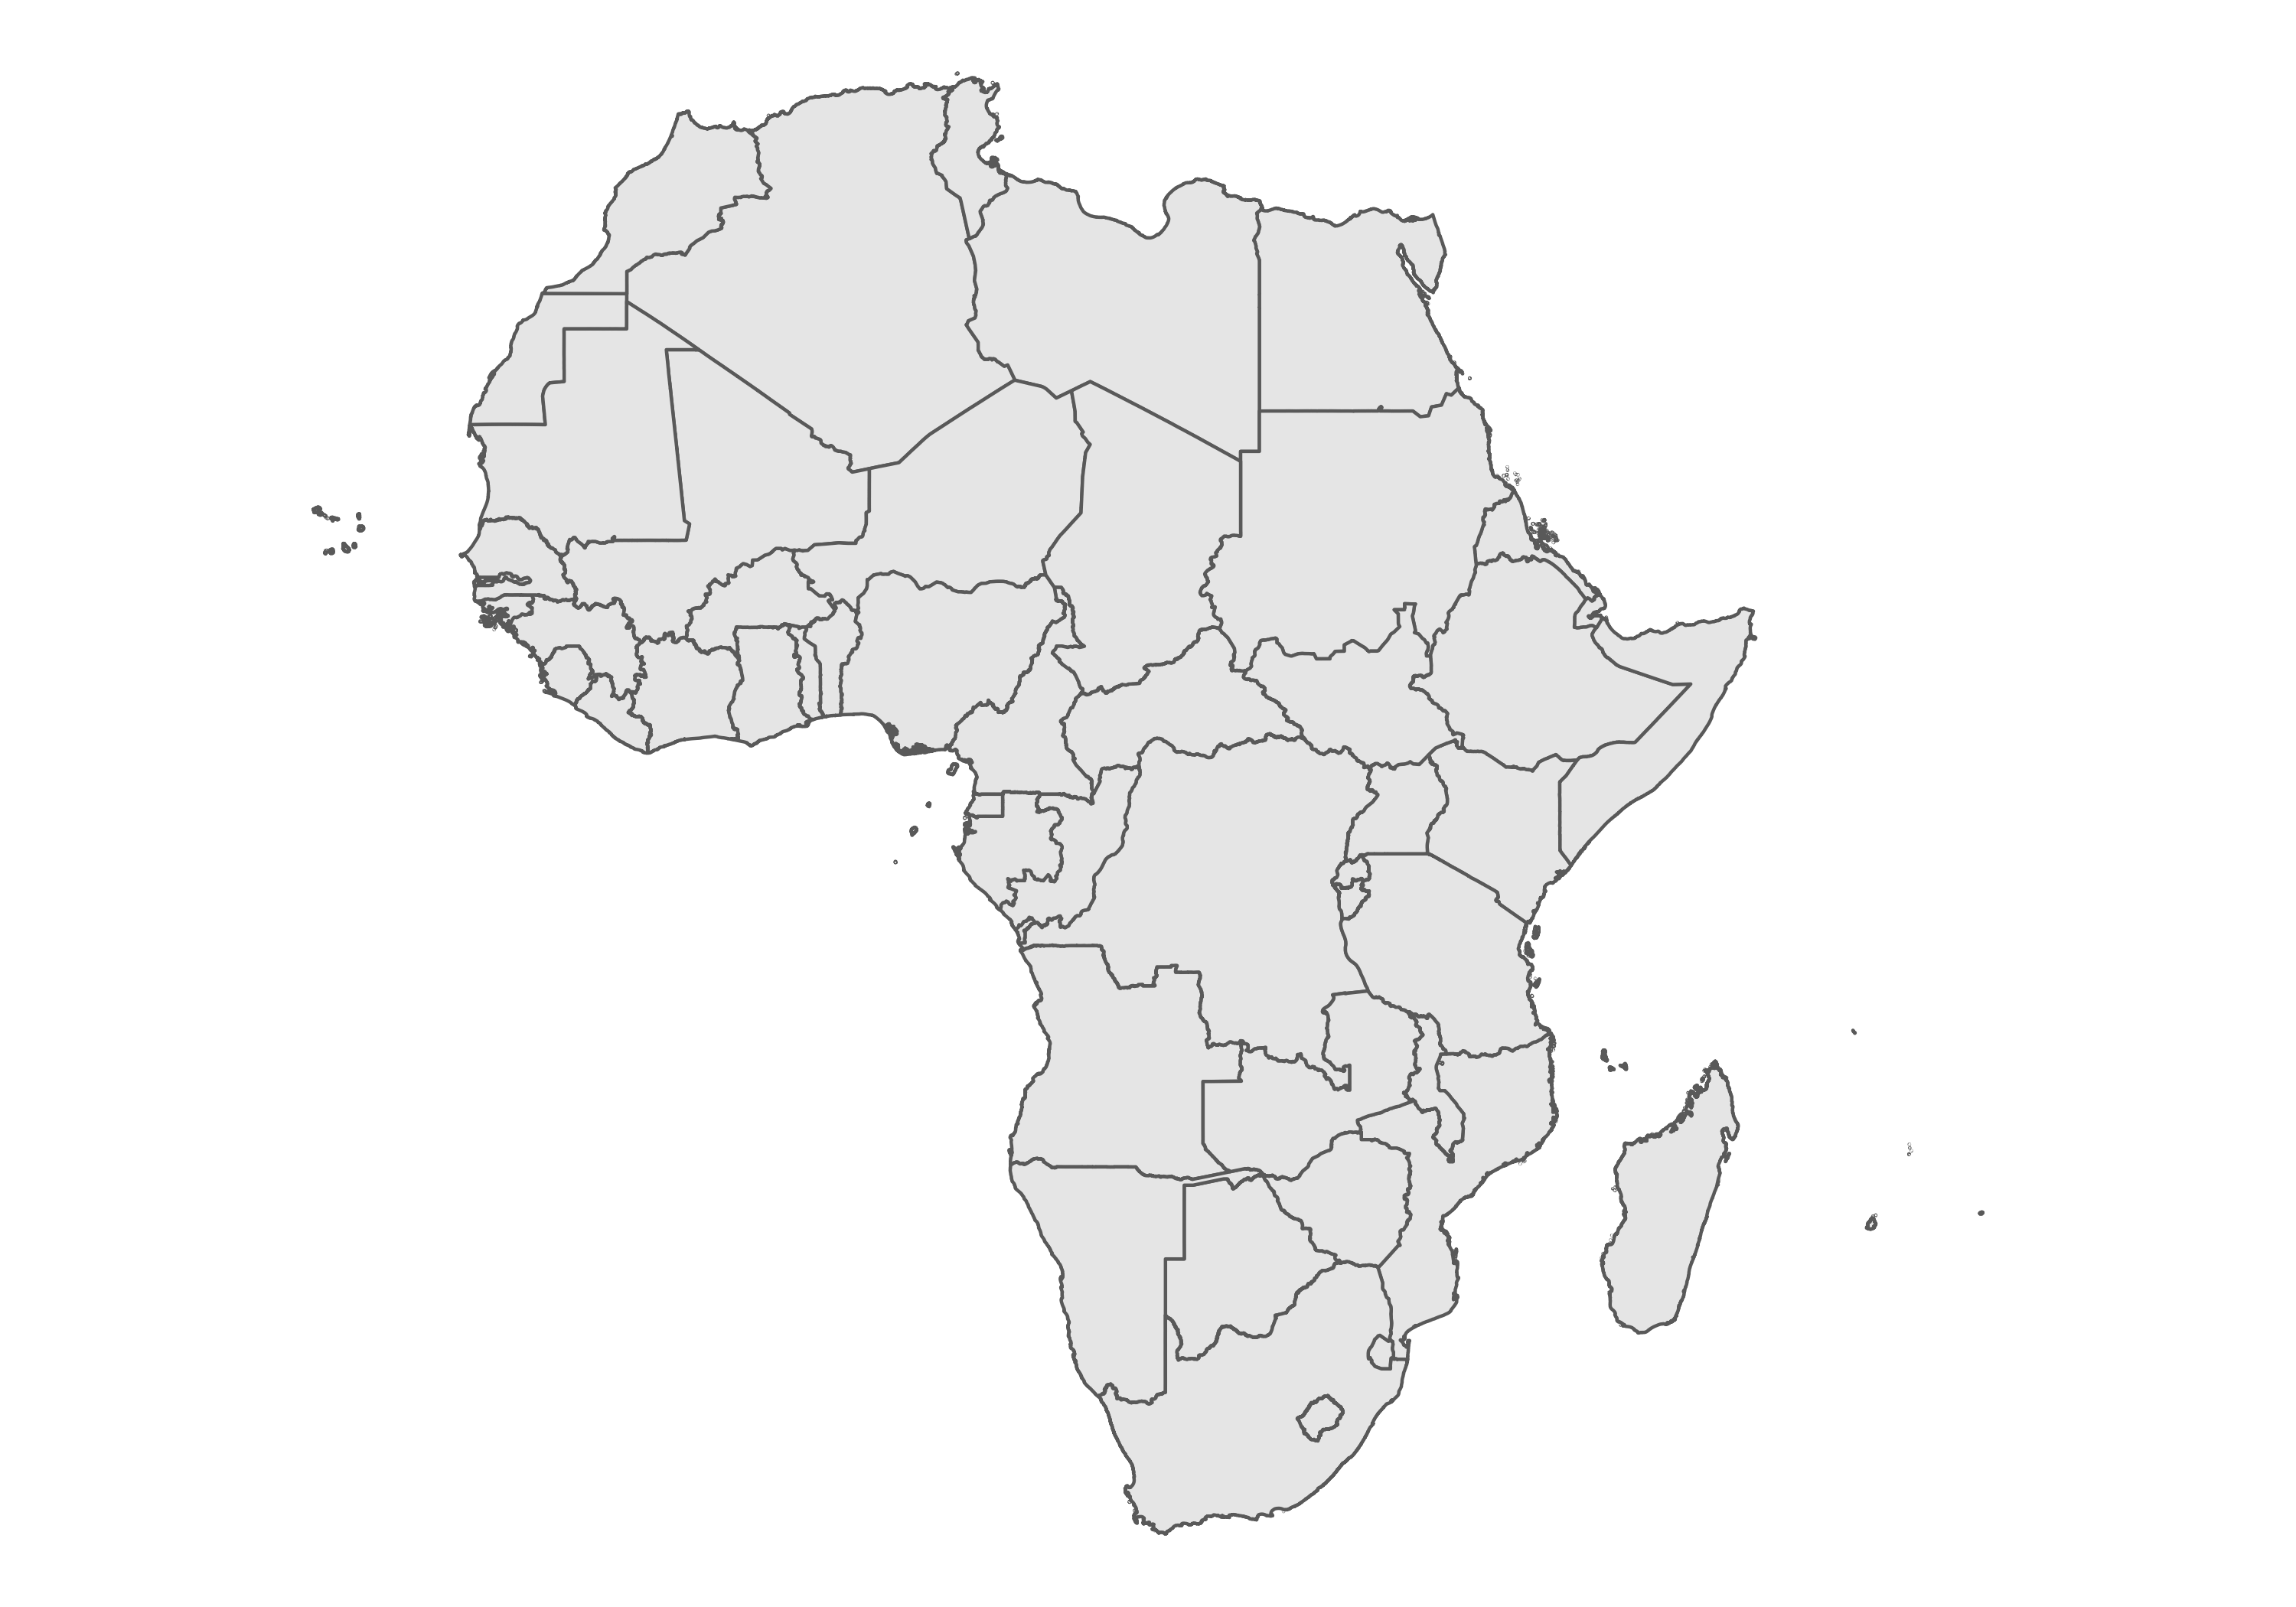
\includegraphics[width=1\textwidth]{figure/g_countries.png}
\end{figure}

\end{frame}



\begin{frame}[fragile]{Find the Centroid of Each Country}{R Code}
\begin{lstlisting}
countries_centroid <- st_centroid(countries)
\end{lstlisting}

\begin{itemize}
	\item Find the centroid of each country using \textbf{st\_centroid()}
	\vspace{0.2cm}
	
\end{itemize}
\end{frame}



\begin{frame}[fragile]{Find the Centroid of Each Country}{R Output}

\begin{figure}
	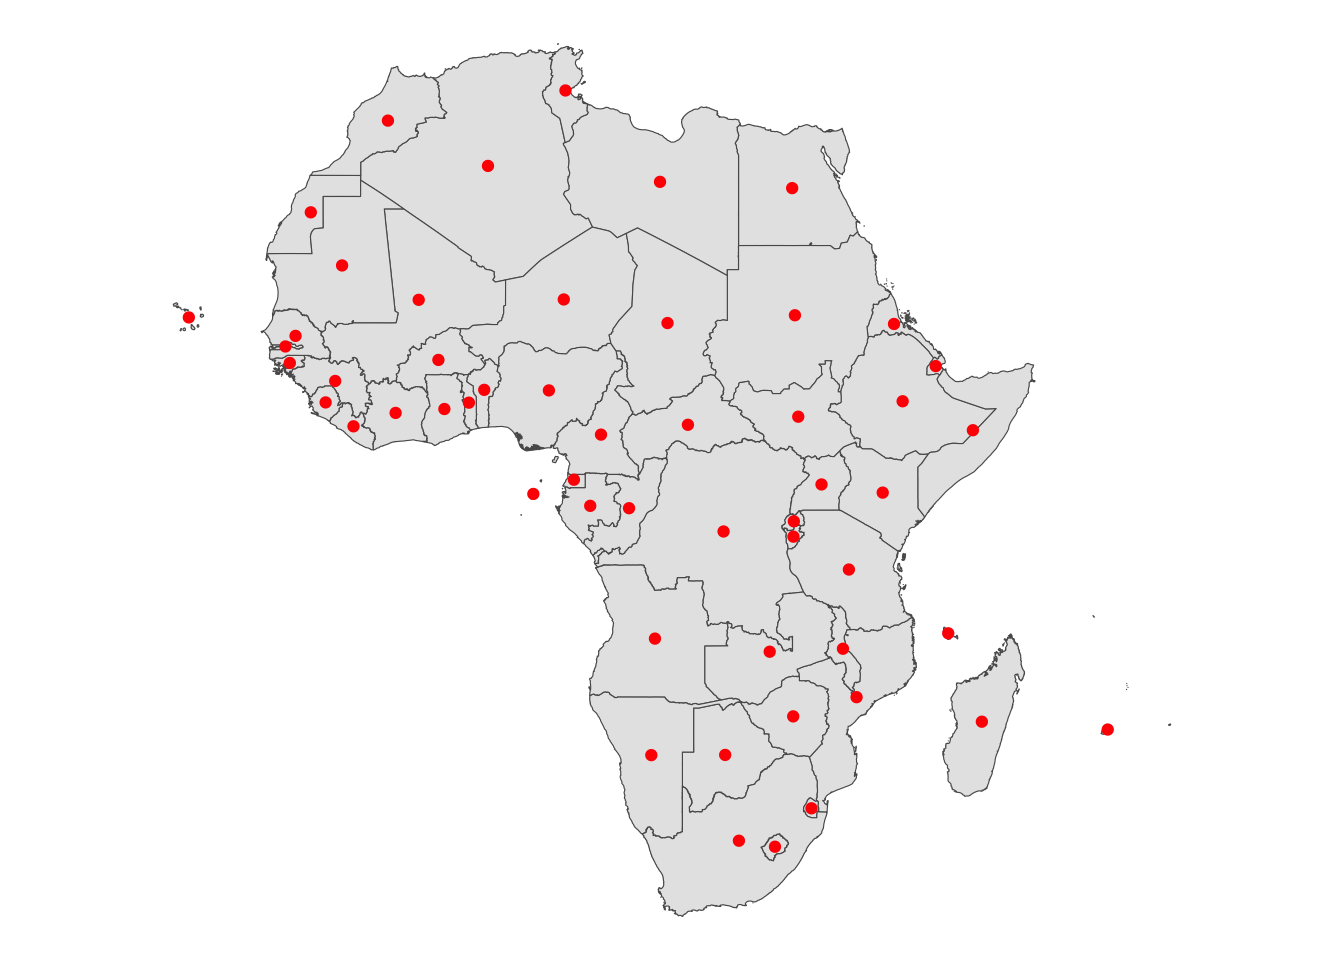
\includegraphics[width=1\textwidth]{figure/centroids-africa-nunn08-1.png}
\end{figure}

\end{frame}





\begin{frame}[fragile]{Nearest Distance between the Centroid and the Coast}{R Code}
\begin{lstlisting}
coast_union <- st_union(coast)
minum_dist_to_coast <- st_nearest_points(countries_centroid, coast_union)
\end{lstlisting}

\begin{itemize}
	\item We find its closest point on the coast line using \textbf{st\_nrearest\_points()}
	\vspace{0.2cm}
	\begin{itemize}
		\item \textbf{st\_nearest\_points(x, y)} loops through each geometry in x and returns the closest point in each feature of y
		\vspace{0.2cm}
	\end{itemize}
\end{itemize}
\end{frame}



\begin{frame}[fragile]{Nearest Distance between the Centroid and the Coast}{R Output}

\begin{figure}
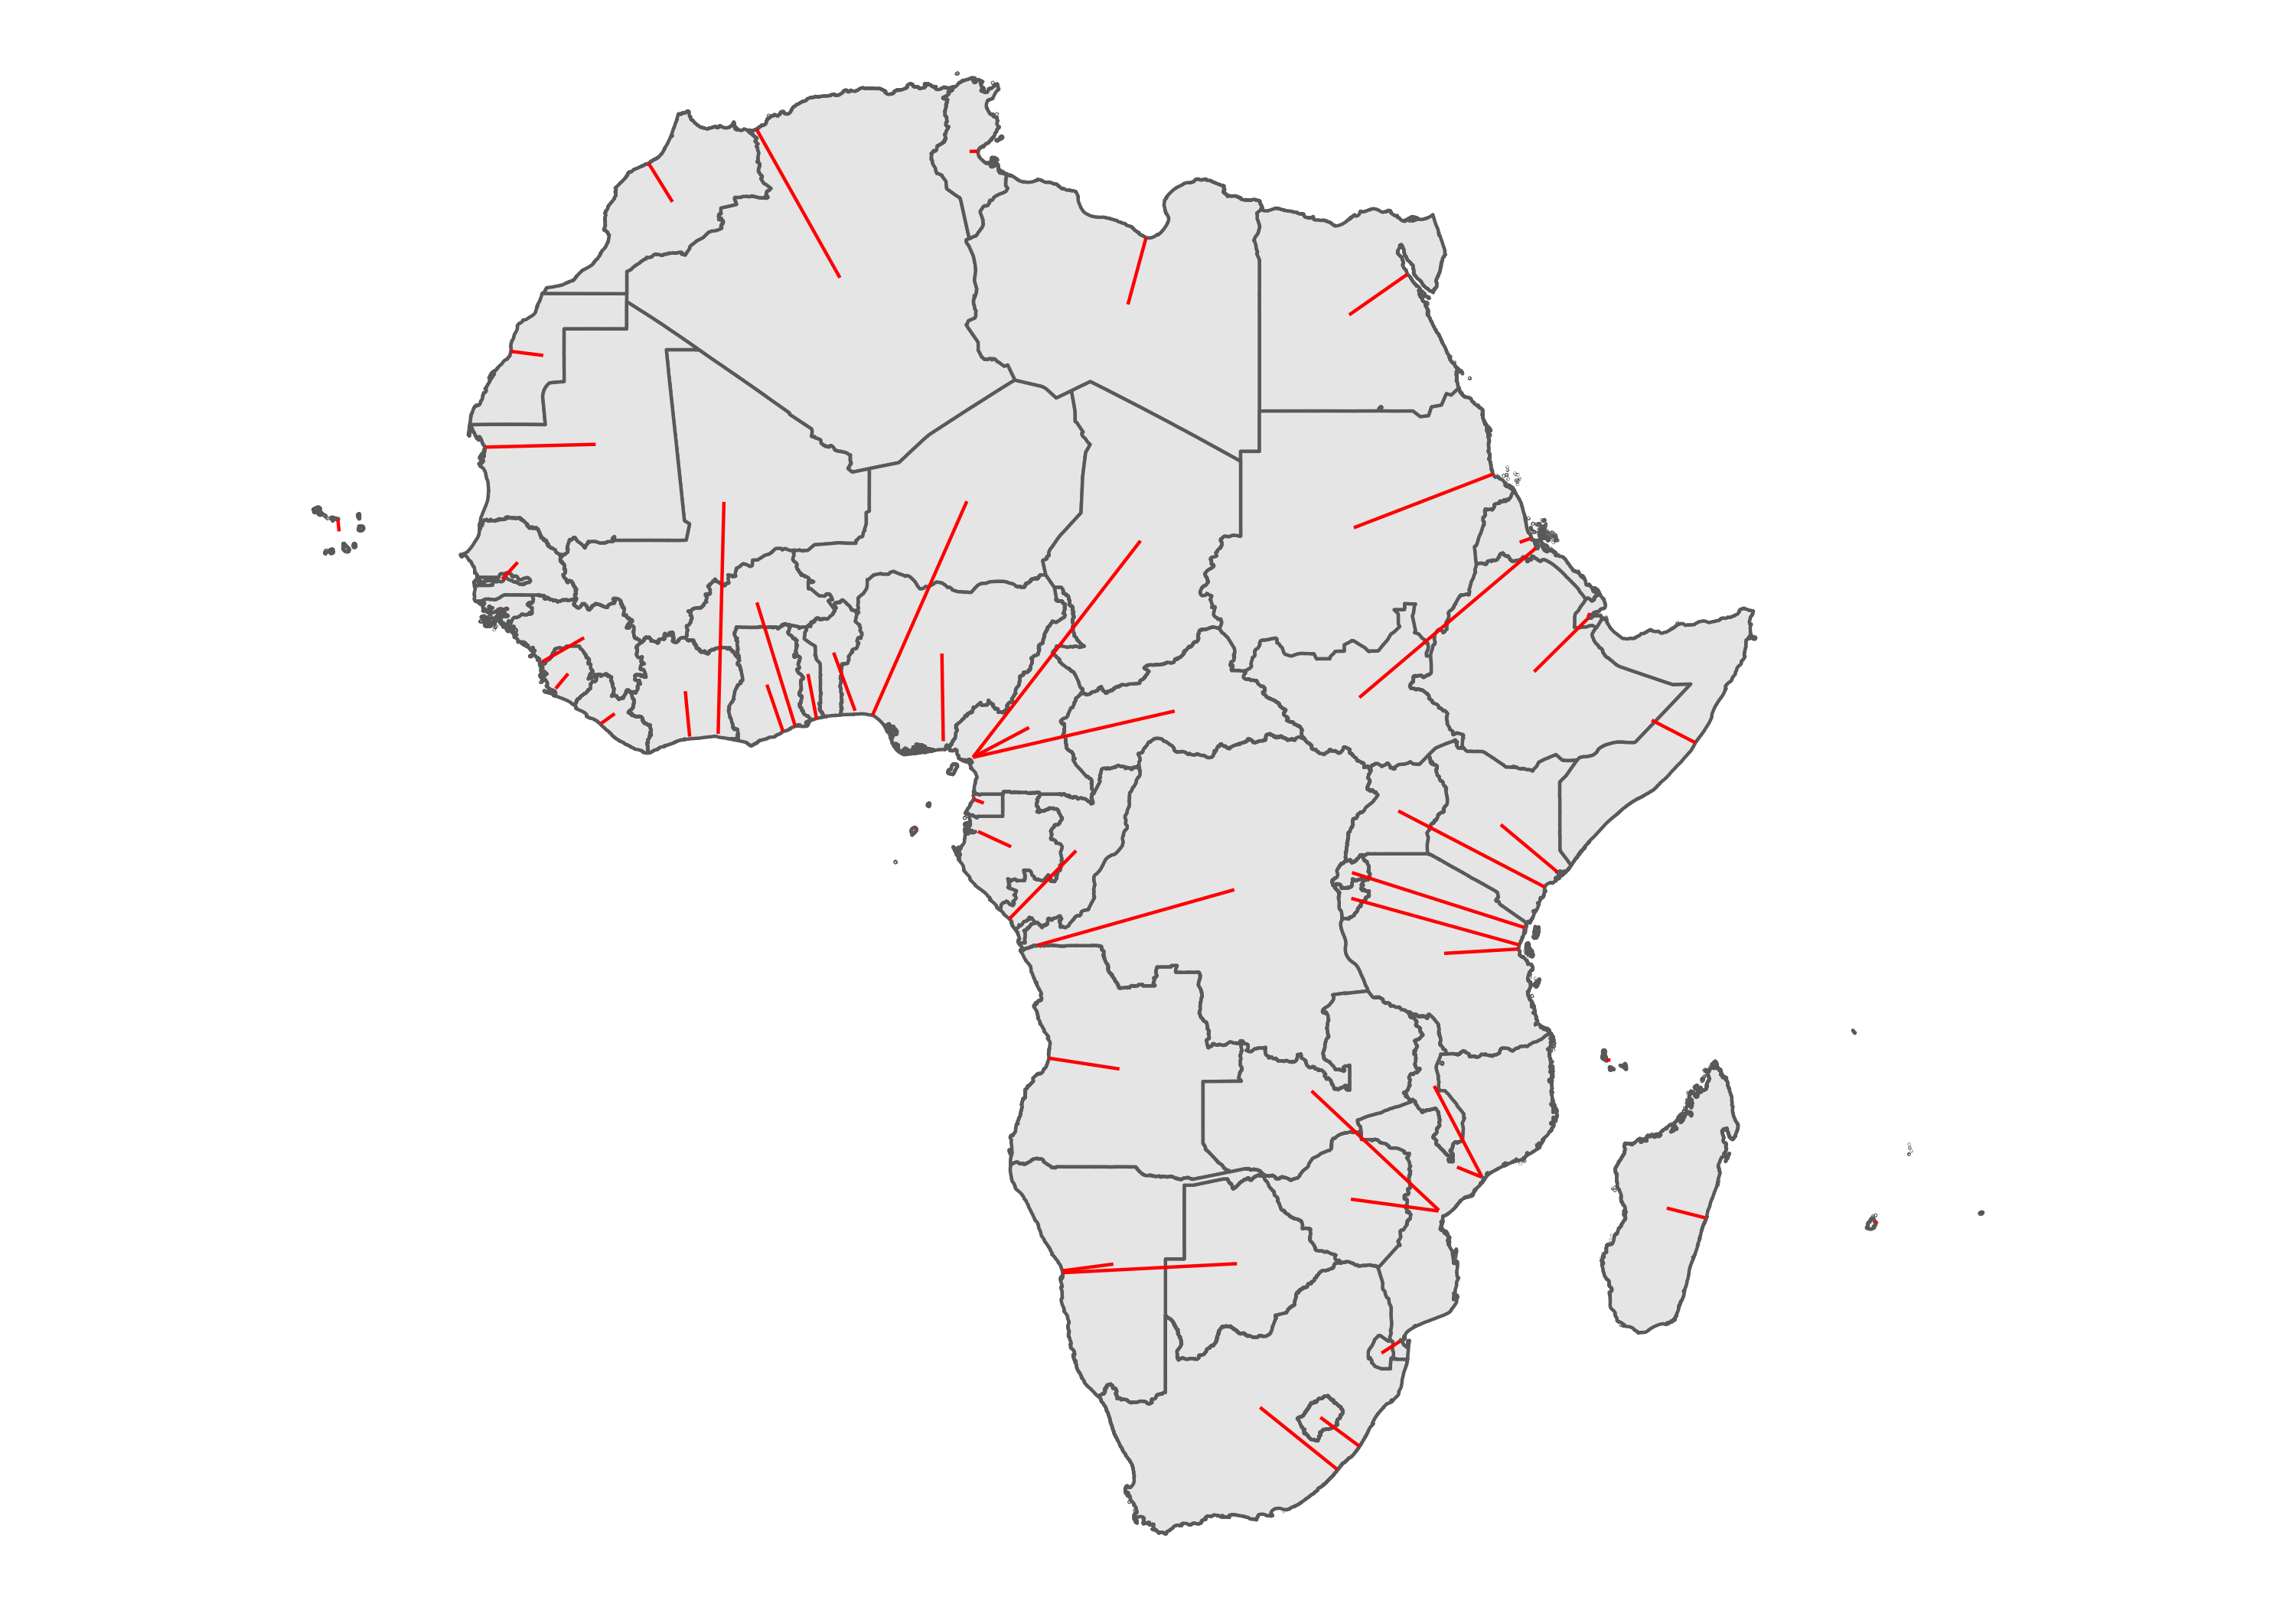
\includegraphics[width=1\textwidth]{figure/g_min_dist_line.png}
\end{figure}

\end{frame}



\begin{frame}[fragile]{Nearest Distance between the Centroid and the Coast}{R Code}
\begin{lstlisting}
closest_pt_on_coast <- lwgeom::st_endpoint(minum_dist_to_coast)
\end{lstlisting}

\begin{itemize}
	\item We can use \textbf{lwgeom::st\_endpoint()} to extract the end point of the lines
	\vspace{0.2cm}
\end{itemize}
\end{frame}



\begin{frame}[fragile]{Nearest Distance between the Centroid and the Coast}{R Output}

\begin{figure}
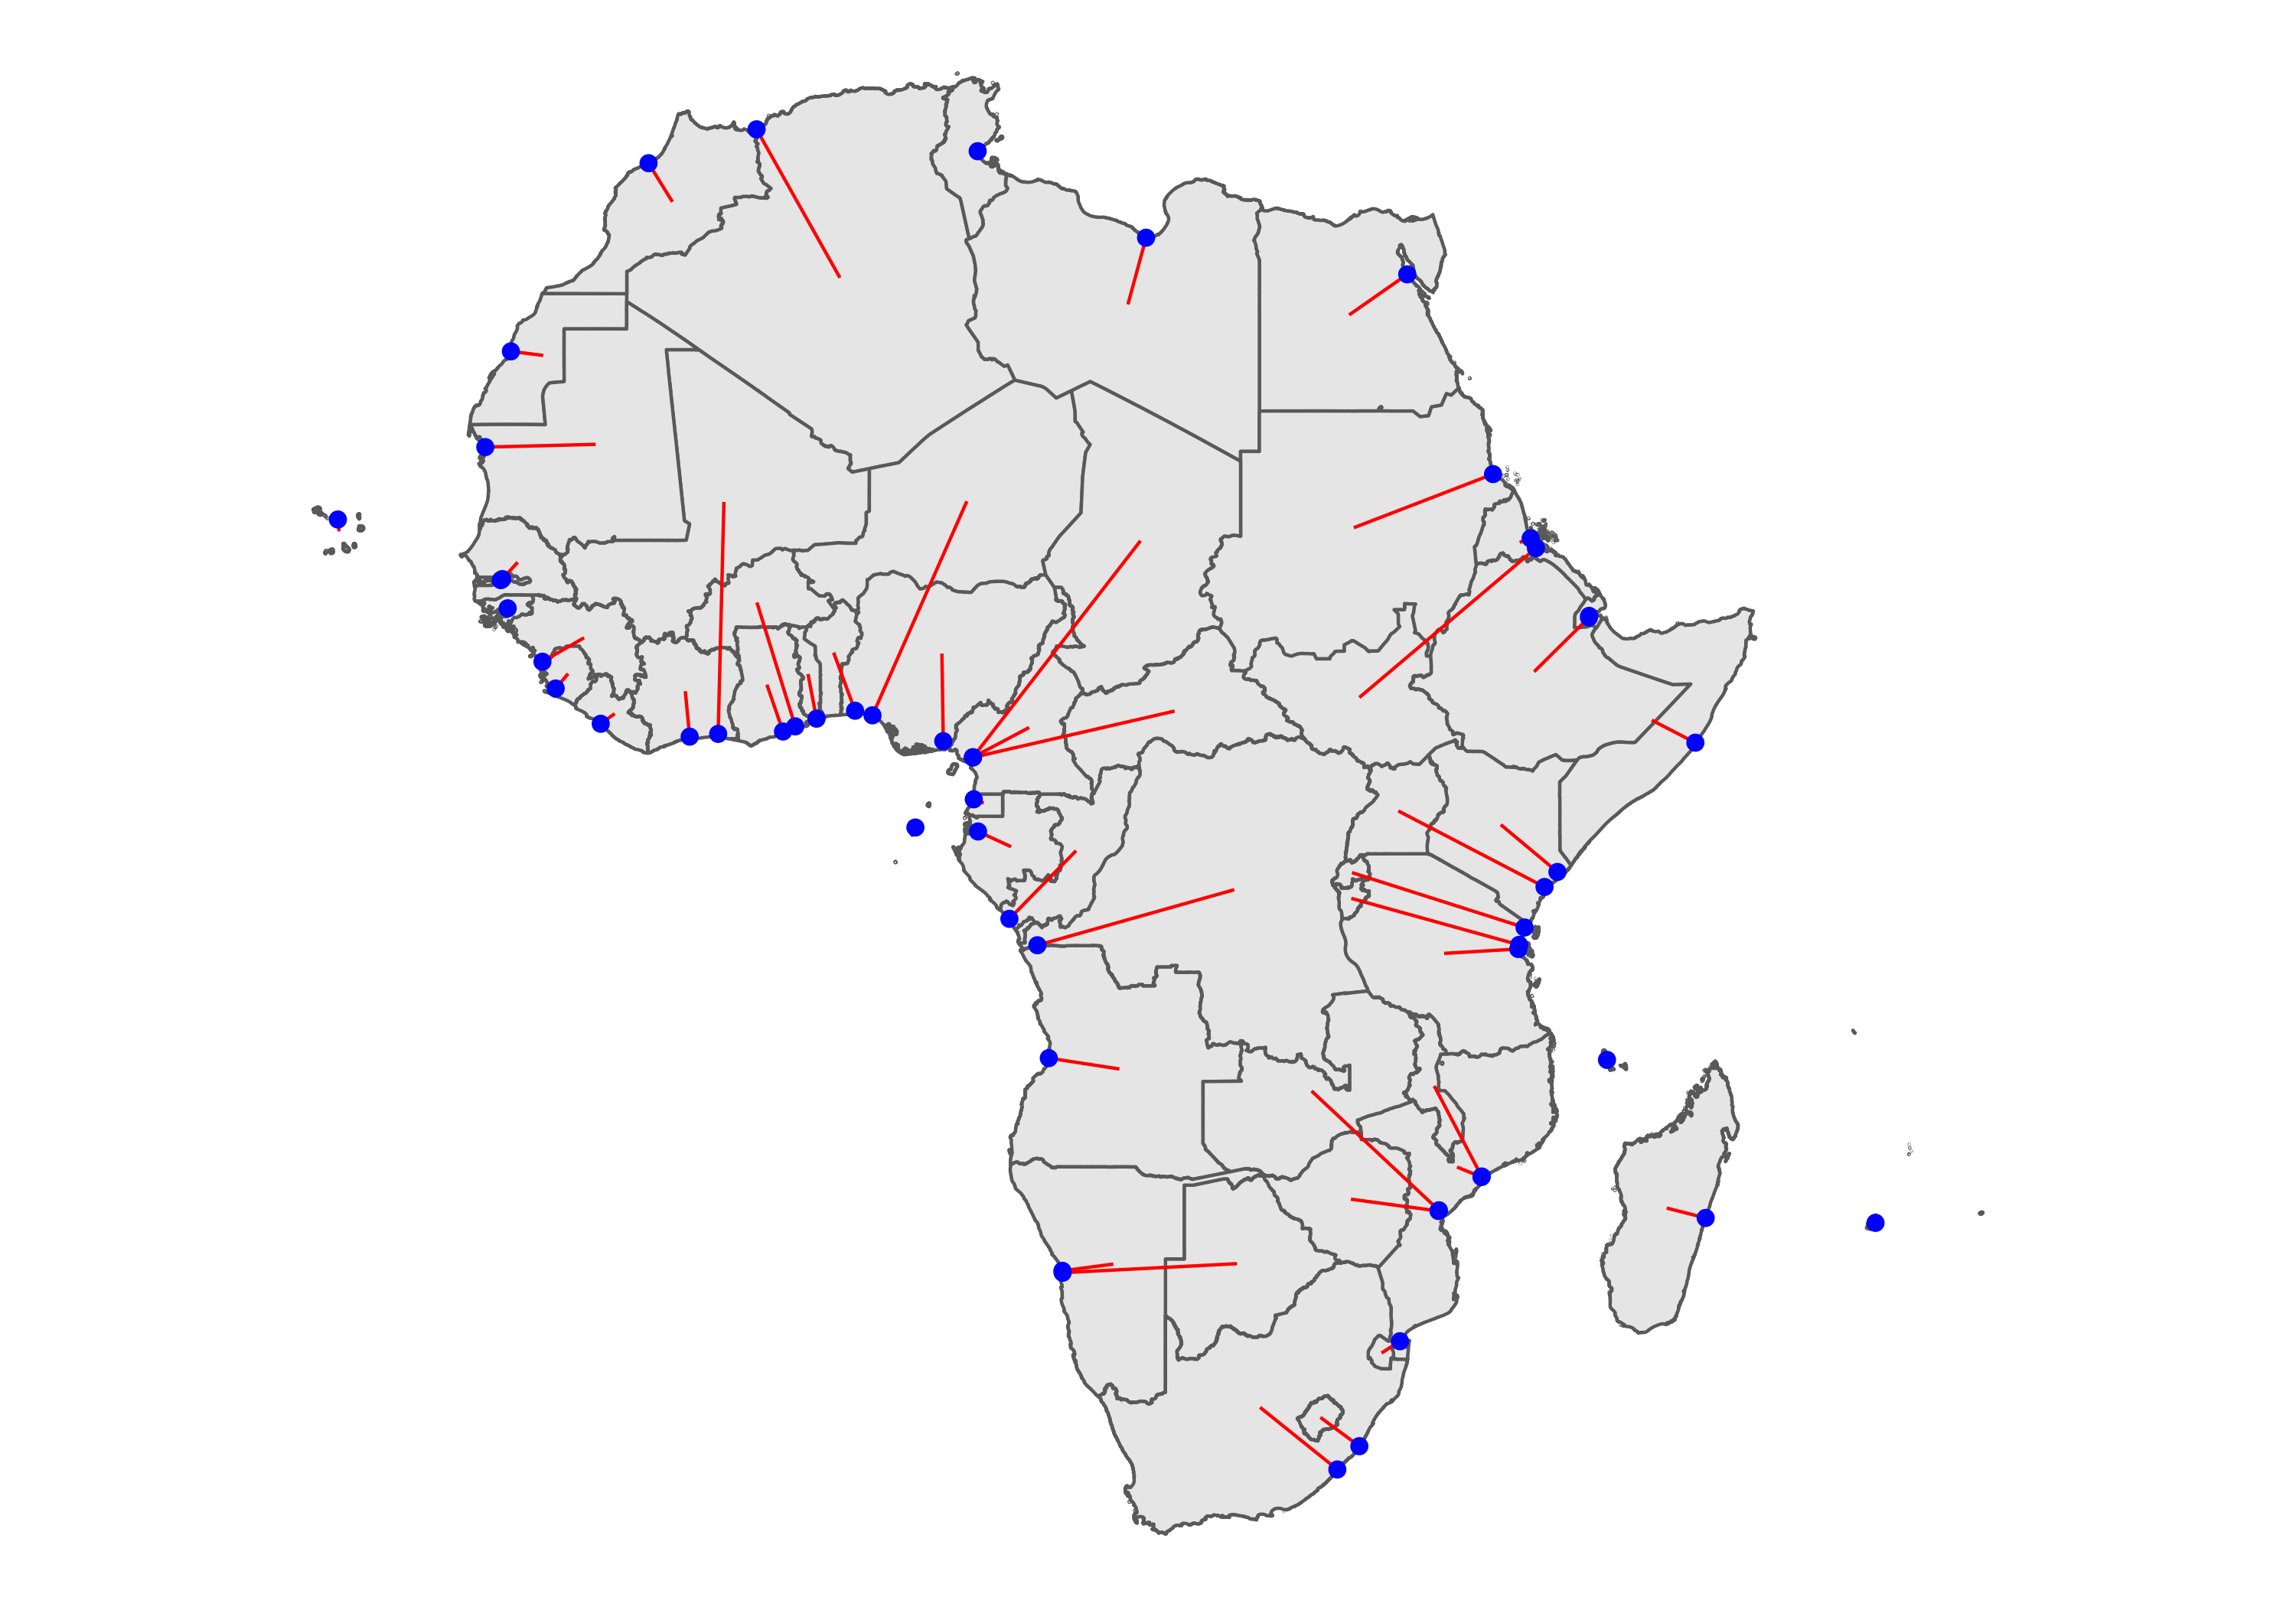
\includegraphics[width=1\textwidth]{figure/g_min_dist_line2.png}
\end{figure}

\end{frame}


\begin{frame}[fragile]{Slave Trade Center}{R Code}
\begin{lstlisting}
trade_centers_sf <-
trade_centers %>%
st_as_sf(coords = c("lon", "lat"), crs = 4326) %>%
st_transform(crs = 3857)
\end{lstlisting}

\begin{itemize}
	\item Convert trade\_centers to an sf object
	\vspace{0.2cm}
	\item Reproejct it to epsg:3857
\end{itemize}
\end{frame}


\begin{frame}[fragile]{Slave Trade Center}{R Output}

\begin{figure}
	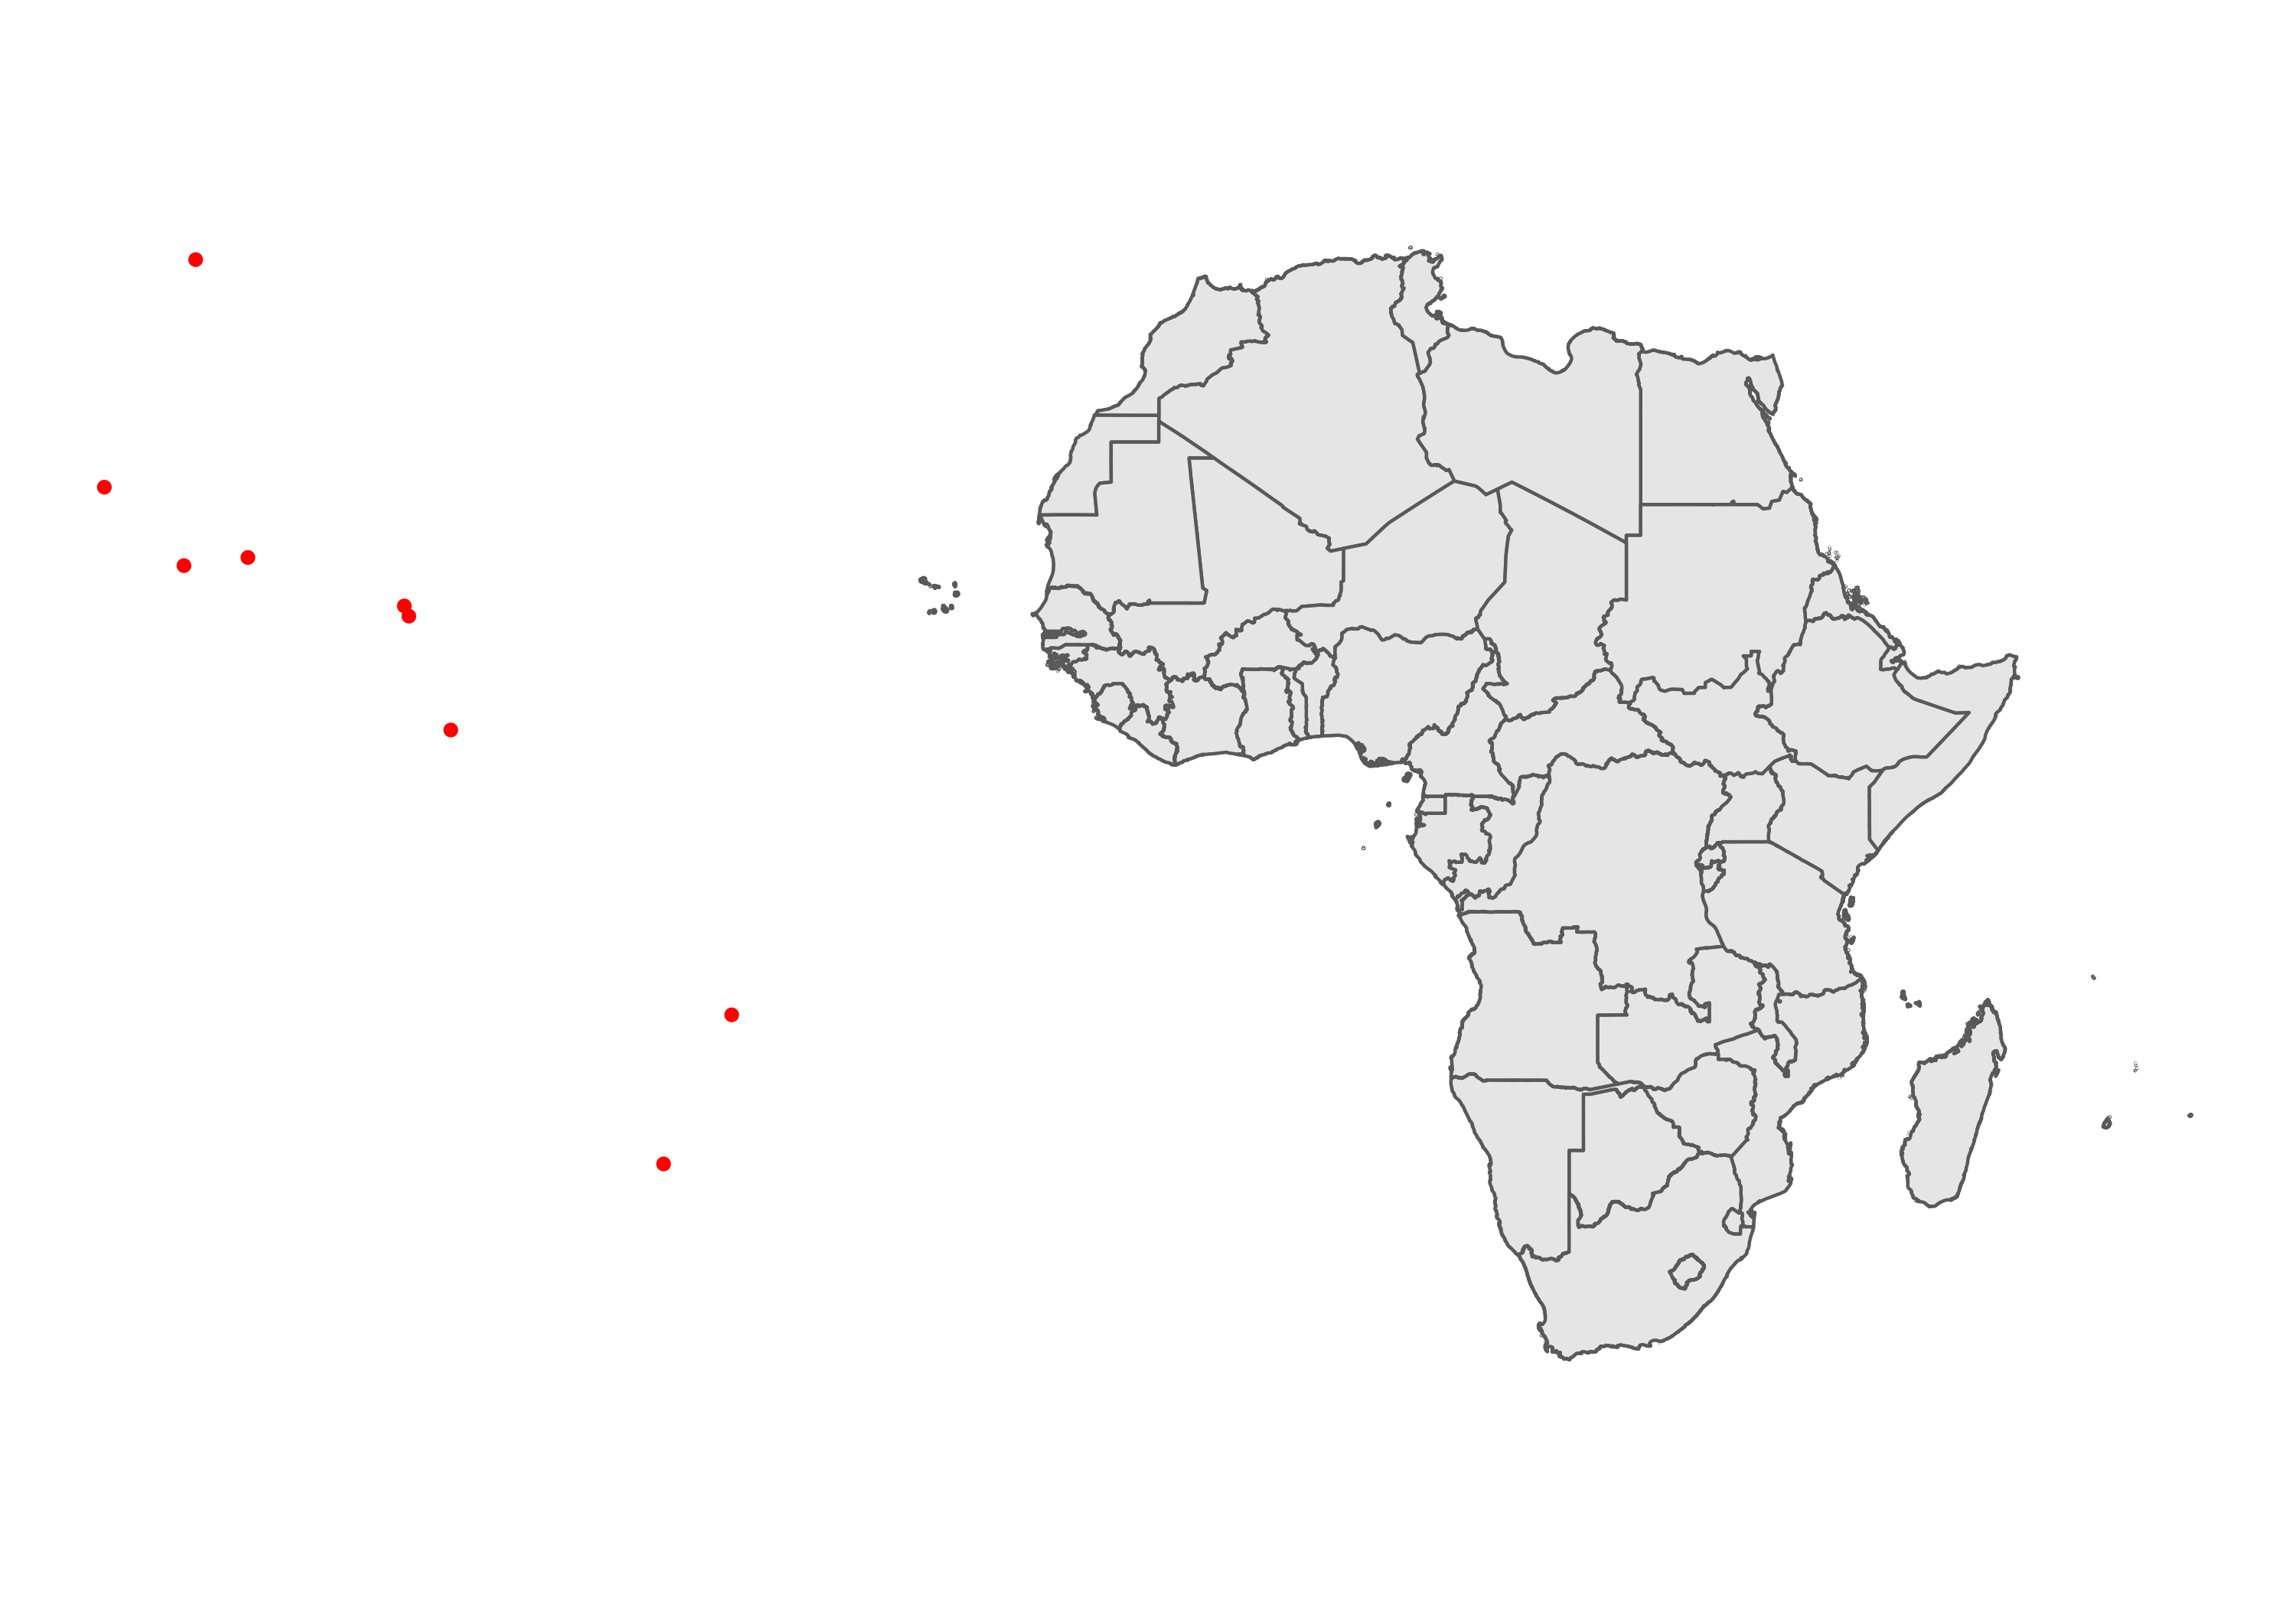
\includegraphics[width=1\textwidth]{figure/trade_centers.png}
\end{figure}

\end{frame}

\begin{frame}[fragile]{Minimum Distance between Trade Center and Country}{R Code}
\begin{lstlisting}
countries_simp$nearest_pt <- closest_pt_on_coast

trade_dist <- st_distance(countries_simp$nearest_pt, trade_centers_sf)

min_trade_dist <- apply(trade_dist, 1, min)
\end{lstlisting}

\begin{itemize}
	\item Get the minimum distance between trade center and African countries
\end{itemize}
\end{frame}



\begin{frame}[fragile]{Minimum Distance between Trade Center and Country}{R Output}

\begin{figure}
	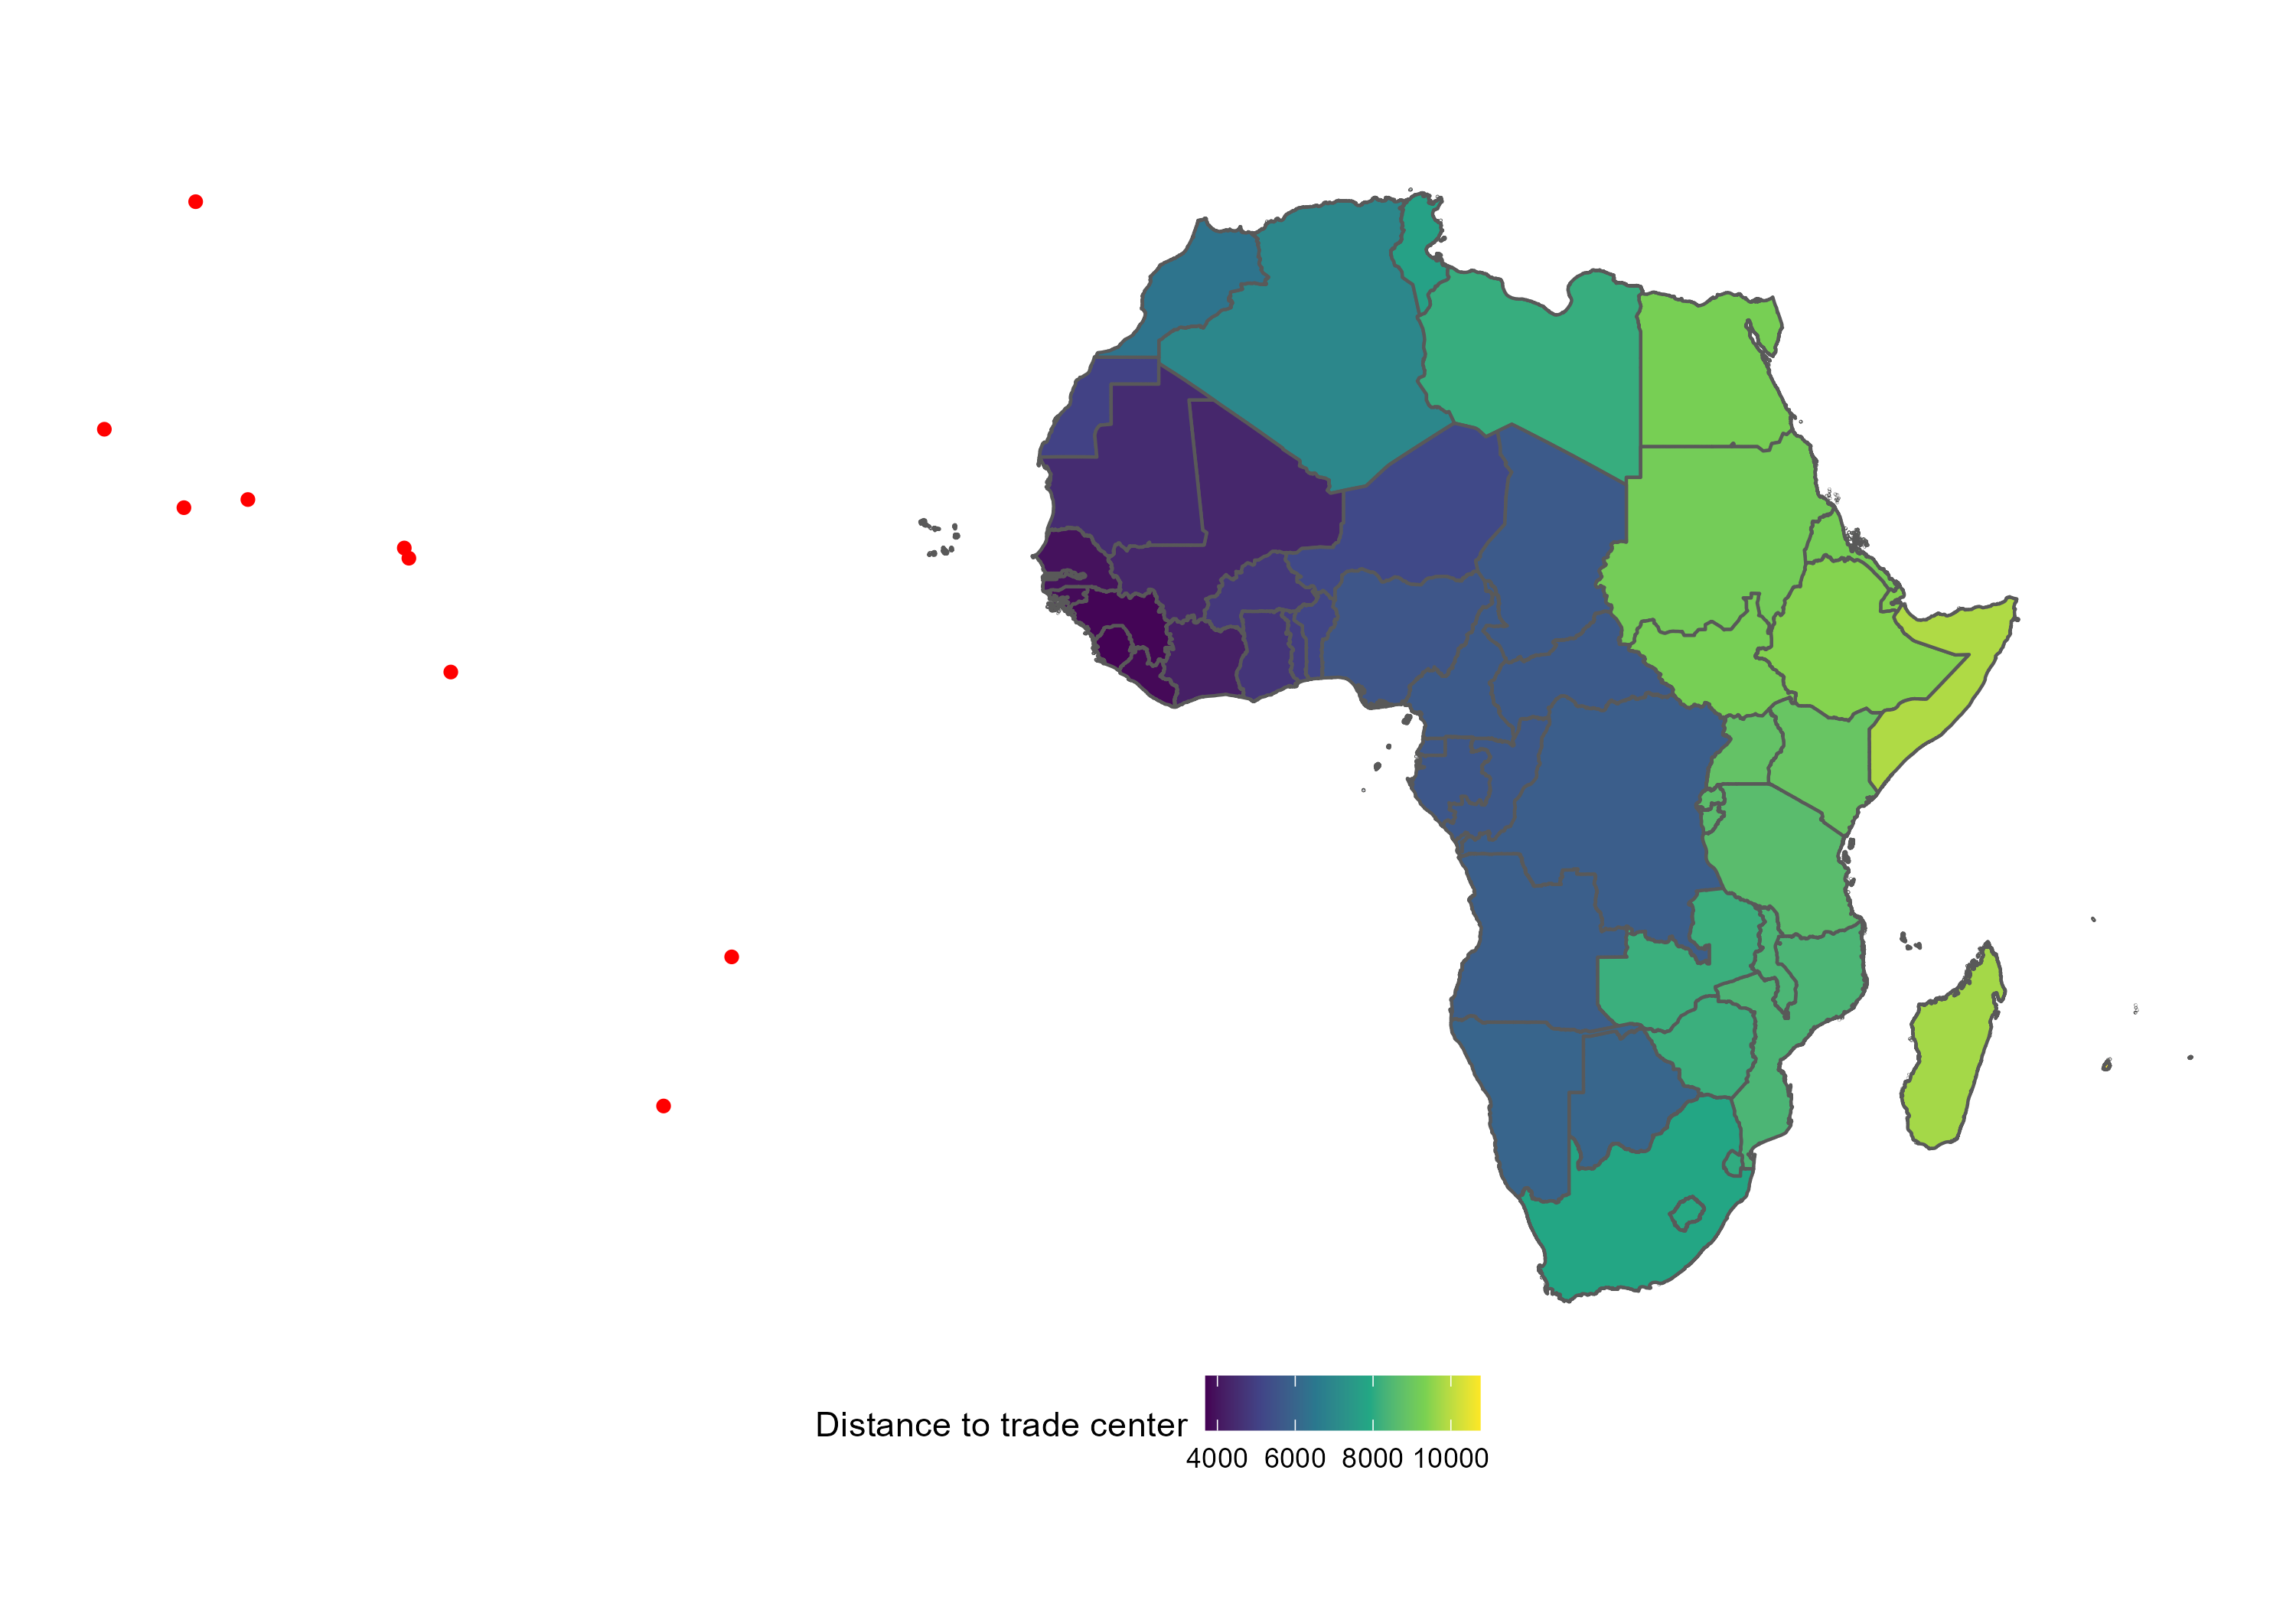
\includegraphics[width=1\textwidth]{figure/min_trade_dist_f.png}
\end{figure}

\end{frame}

\end{document} 
